\documentclass[twocolumn]{svjour3}
\usepackage{graphicx}
\usepackage{amsmath}
\usepackage[colorlinks=true,linkcolor=blue,citecolor=blue,urlcolor=blue]{hyperref}
\begin{document}
\title{A Machine Learning Based Framework for Predictive School Management Using Student and Faculty Analytics}
\author{Ming Yang \and Zhe Li \and Shaoyan Liu}
\institute{Ming Yang \at 1Department of Science and Education, Aviation General Hospital, No. 3, Beiyuan Road, Chaoyang District, Beijing, 100012, China, \email{13718330851@163.com} \and Zhe Li \at 2Discipline Inspection Office, Capital Medical University Affiliated Beijing Hospital of Traditional Chinese, Beijing, 100010, China \and Shaoyan Liu \at 3Department of Educational Teaching Quality Construction, Chinese Research Academy of Traditional Chinese Medicine College, Beijing, 100700, China}
\journalname{Scientific Reports}
\date{2026}
\maketitle
\begin{abstract}
New technologies in education have created a huge amount of data that, when used effectively, can have a major impact on the functioning of an institution and the academic achievement of students. Nevertheless, all existing predictive models are still disconnected and do not integrate historical trends, student-faculty relationships, and trend patterns into a coherent decision-making system. The paper describes an integrated machine learning system that integrates several synergistic AI technologies: (1) deep learning systems (LSTM, GRU, CNN, and Transformers) to model academic growth over time; (2) comprehensible gradient boosting ensembles (XGBoost, LightGBM, and CatBoost) to understandably infer and analyze structured data. (3) graph convolutional networks (GCNs) to encode academic relationships between students, professors, and courses; and (4) data-centric oriented approaches (multitasking, transfer, and federated learning). The framework is tested on two UCI benchmark datasets (n=649) with fully isolated holdout sets using strict nested cross-validation to prevent data leakage. The framework yields 99.6\% and 97.5\% predictive accuracy (5.6\% and 6.3\% improvement over the top baselines) and high recall (99.4\% and 96.7\%) in classifying at-risk students. Each component has been shown to contribute fully in ablation studies, and the hybrid framework has been table models shown (TabTransformer, FT-Transformer, and SAINT) (99.6\% vs. 97.2\% for the best transformer). Robustness analysis with feature noise and missing data (>96\% accuracy with 20\% missing data) demonstrates excellent regression. Fairness assessment indicates that gender and age bias are very small, and mitigation 
to outperform 
state-of-the-art 
transformed
\keywords{Predictive Educational Analytics, Hybrid Deep Learning, Graph Neural Networks (GNNs), Ensemble Methods, Student At-Risk Identification, Intelligent School Management Systems}
\end{abstract}
% ===== MAIN DOCUMENT CONTENT =====

\section{Advanced Deep Learning Methods for Predictive Educational Modeling}
In an advanced deep learning method, Sudhamathy and Valliammal et al. (2023) created a uniform Bayesian CNN-LSTM learning performance prediction model and demonstrated an accuracy of 98.18\%, a precision of 97.09\%, a recall of 96.38\%, and an F1-score of 95.35\%, which was better than using LSTM alone \cite{13}. Similarly, Elrahman et al. (2023) implemented a CNN-BiLSTM-Random Forest hybrid that achieved an accuracy of 77\%, a precision of 0.72, a recall of 0.68, and an F1-score of 0.69, supporting the value of hybrid deep learning for academic forecasting \cite{14}. 
The author Zhang et al. (2025) developed a convolutional neural network, long short-term memory (CNN-LSTM) architecture for the prediction of Massive Open Online Courses (MOOCs) and achieved an accuracy of 93.41\% with 87.71\% precision, 85.42\% recall, and an 89.06\% F1-score. This was shown to be better than Random Forest models \cite{15}. Kumar et al. (2025) noted LSTM achieved an accuracy of 91.5\% with a precision of 89.7\% and a recall of 88.3\% for the prediction of sports injury; they confirmed LSTM was the best model for predicting sports injury over GRU and CNN models \cite{16}. 
With regard to ensemble learning, Selvaraj et al. (2024) compared two algorithms, CatBoost and XGBoost, for diabetes prediction. Both models achieved classification accuracy corresponding to ~91.08\% and ~88.33\% for CatBoost and XGBoost, respectively, as well as F1-scores of 87.38\% and 86.5\%. CatBoost outperformed XGBoost in both accuracy and F1-scores \cite{17}. In a similar study, Cheng et al. (2025) noted CatBoost outperformed XGBoost with an accuracy of 96.09\% and an F1-score of 92.13\% \cite{18}. 
The author Chella et al. (2024) compared a number of ML models with regard to student analytics; they considered the Decision Trees, Random Forest, and XGBoost, finding that XGBoost performed the best with an accuracy of ~90\% and the most balanced F1-scores, as it outperformed both traditional statistical models \cite{19}. 
In a related study, Nadar et al. (2023) proposed a Modified XGBoost (MXGB) algorithm using the stream data analysis process, noting it yielded improved accuracy ($\approx$92\%), precision ($\approx$90\%), and F1-score ($\approx$89\%), indicating it was a sufficient algorithm for predicting student performance in real-time \cite{20}. A recommendation system powered by AI was created by Herath and others (2024), incorporating Random Forest, SVM, CatBoost, and XGBoost, where Random Forest recorded the best scores with 94\% accuracy, 91\% precision, 90\% recall, and 91\% F1-score, thereby supporting its use toward personalized learning strategies \cite{21}. 
Borna et al. (2024) ran AI models on clickstream data, which recorded 78.68\% accuracy using Random Forest, supporting the increasing role of ML in adaptive educational assessments \cite{22}. Moreover, hybrid DL, and DL-ensemble models have been validated in more general predictive contexts. M. Balayet Hossain Sakil et al. (2025) created a CNN-Transformer-XGBoost model, which achieved a 92\% test F1-score and a 97\% AUC to show its superiority to LightGBM and CatBoost for healthcare fraud detection \cite{23}. Dritsas and Trigka et al. (2024) similarly showed that a hybrid deep learning model of CNN, RNN, and GRU achieved 91\% accuracy, 89\% precision, 90\% recall, and an 89\% F1-score in predicting heart attacks \cite{24}.
\begin{table}[htbp]
\centering
\caption{Summary of Related Work on ML/DL Techniques for Predictive Educational and Hybrid Modeling}
\label{tab:1}
\begin{tabular}{lll}
\hline
Author & Ref & Dataset Context \\
\hline
Gurcan et al. [11] & Case-Based & XGBoost, Random \\
& & Performance Metrics (Acc, Prec, Rec, F1) \\
& & Acc: 95.23\%, Prec: \\
& & Educational Data Mining (EDM) \\
& & Decision Trees (CART), \\
& & Ensemble Learning, \\
& & Key Limitation \\
& & Contribution to Justifying Hybrid Model \\
& & Focuses narrowly on balanced CBL data; results may degrade \\
& & Supports XGBoost's high single-model \\
\hline
\end{tabular}
\end{table}

\section{Learning (CBL)}
\subsection{Forest, AdaBoost}
95.38\%, Rec: 95.23\%, F1: 95.23\%
\subsection{Random Forest}
\subsection{Predictive Analytics}
on highly imbalanced real-world data.
\subsection{Laribi \& Gaceb \cite{12}}
Student Dropout Risk
\subsection{XGBoost}
Acc: 91,Prec: 88\%,F1: 81\%
\subsection{Naïve Bayes, Logistic Regression}
\subsection{Classification, Dropout Risk Analytics}
\subsection{Sudhamathy \& Valliammal \cite{13}}
Learning Performance Prediction
\subsection{Uniform Bayesian CNN-LSTM}
Acc: 98.18\%, Prec: 97.09\%, Rec: 96.38\%, F1: 95.35\%

\section{Sequential Pattern Mining}
\subsection{Deep Learning Sequence Modeling}
Elrahman et al. \cite{14}
\section{Academic Forecasting}
Zhang et al. \cite{15}
\section{MOOCs Prediction}
\subsection{CNN-BiLSTM-Random Forest hybrid}
\subsection{CNN-LSTM architecture}
Acc: 77\%, Prec: 0.72, Rec: 0.68, F1: 0.69
\section{Bayesian Knowledge Tracing (BKT)}
\subsection{Time-Series Forecasting}
Acc: 93.41\%, Prec: 87.71\%, Rec: 85.42\%, F1: 89.06\%
\section{Sequential Pattern Mining}
\subsection{Learning Behavior Analytics}
Kumar et al. \cite{16}
\section{Sports Injury Prediction}
\subsection{LSTM (vs GRU, CNN)}

\section{LSTM (vs GRU, CNN)}
\begin{table}
\centering
\caption{Performance Metrics}
\begin{tabular}{lll}
\hline
Metric & Value & Unit \\
\hline
Accuracy & 91.5\% & \% \\
Precision & 89.7\% & \% \\
Recall & 88.3\% & \% \\
\hline
\end{tabular}
\end{table}
\section{Bayesian Knowledge Tracing}
\section{Time-Series Analysis}
\subsection{Selvaraj et al. [17]}
\section{Diabetes Prediction}
\subsection{CatBoost vs. XGBoost}
\begin{table}
\centering
\caption{Performance Metrics}
\begin{tabular}{lll}
\hline
Model & Accuracy & F1 \\
\hline
CatBoost & 91.08\% & 87.38\% \\
XGBoost & 88.33\% & 86.5\% \\
\hline
\end{tabular}
\end{table}
\section{Association Rule Mining}
\subsection{Gradient Boosting, Ensemble Methods}
\subsection{Cheng et al. [18]}
\section{General Classification}
\subsection{CatBoost (vs XGBoost)}
\begin{table}
\centering
\caption{Performance Metrics}
\begin{tabular}{lll}
\hline
Model & Accuracy & F1 \\
\hline
CatBoost & 96.09\% & 92.13\% \\
\hline
\end{tabular}
\end{table}
\section{Decision Trees}
\subsection{Chella et al. [19]}
\section{Student Analytics}
\subsection{Decision Trees, Random Forest, XGBoost}

\section{Decision Trees, Random Forest, XGBoost}
\subsection{Acc: ~90\%}
\subsection{ID3, CART}
\subsection{Structured Data Classification}
\subsection{Predictive Educational Modeling}
High precision indicates good detection of at-risk students, but the lower F1 suggests some trade-off with recall.
\subsection{Hybrid DL-based approach is complex and computationally expensive; superior performance is noted only against LSTM alone.}
\subsection{Accuracy and F1-score are comparatively lower, indicating performance sensitivity to the specific dataset or feature engineering challenges.}
\subsection{Bested Random Forest, but still shows a gap between high accuracy and recall/precision, suggesting challenges with class imbalance.}
\subsection{High performance is noted, but this is a non-educational context; applicability to academic data needs validation.}
\subsection{Non-educational context. The comparison is critical for selecting the optimal boosting algorithm for the Ensemble Pillar.}
\subsection{Non-educational context. Reinforces CatBoost's superiority in general structured prediction problems.}
\subsection{Directly supports XGBoost's high performance in educational analytics, outperforming other common ML models.}
\subsection{efficacy on structured, balanced educational data. Validates XGBoost as a strong tool for binary classification tasks like dropout prediction in education. Demonstrates superiority of hybrid Deep Learning models over single DL models (LSTM) for capturing complex patterns.}
\subsection{Supports the value of DL-Ensemble Hybrids for time-series/sequential data, despite variable performance based on data.}
\subsection{Confirms the effectiveness of CNN-LSTM for sequential/time-series data and its advantage over traditional ensembles in that context. Reinforces LSTM's effectiveness for time-series forecasting and its potential as a component in sequential learning. CatBoost outperforms XGBoost, justifying its selection or co-use in the Ensemble Pillar for maximizing accuracy on structured data.}
\subsection{Further evidence supporting CatBoost's high accuracy for the Ensemble Pillar.}
\subsection{Confirms XGBoost's robustness as a core component of the Ensemble Pillar in the educational domain.}

\section{Confirms XGBoost's robustness as a core component of the Ensemble Pillar in the educational domain.}
\subsection{Student Performance (Real-Time)}
\subsubsection{Modified XGBoost (MXGB)}
Acc: \textbf{$\approx$}92\%, Prec: \textbf{$\approx$}90\%, F1: \textbf{$\approx$}89\%
\subsection{Stream Mining}
\subsubsection{Real-Time Data Analytics}
Herath et al. \cite{Herath et al. [21]}
\subsection{Recommendation System}
Random Forest, SVM, CatBoost, XGBoost
Acc: 94\%, Prec: 91\%, Rec: 90\%, F1: 91\%
\subsection{K-Means, Association Rules}
\subsubsection{Personalized Learning Recommendations}
Borna et al. \cite{Borna et al. [22]}
\subsection{Adaptive Educational Assessments (Clickstream Data)}
Random Forest
Acc: 78.68\%

\section{Sequential Pattern Mining}
\subsection{Clickstream Behavioral Analysis}
Sakil et al. \cite{23}
\subsection{Healthcare Fraud Detection}
CNN-Transformer-XGBoost
\begin{table}
\centering
\caption{Performance Metrics}
\begin{tabular}{lll}
\hline
F1 & AUC & Acc \\
\hline
92\% & 97\% & 78.68\% \\
\hline
\end{tabular}
\end{table}
\subsection{Hybrid Deep Learning + Ensemble}
Dritsas \& Trigka \cite{24}
\subsection{Heart Attack Prediction}
CNN, RNN, and GRU Hybrid
\begin{table}
\centering
\caption{Performance Metrics}
\begin{tabular}{lll}
\hline
Acc & Prec & Rec & F1 \\
\hline
91\% & 89\% & 90\% & 89\% \\
\hline
\end{tabular}
\end{table}
\subsection{Sequential Temporal Modeling}
Modifying core algorithms (MXGB) is necessary to achieve better performance on stream data (real-time).
Random Forest (RF) is best for personalized learning recommendations, a task distinct from direct performance prediction.
Lower accuracy suggests challenges in extracting predictive signals from raw behavioral (clickstream) data alone.
Non-educational context. Hybrid model demonstrates success in capturing complex features and robust prediction.

\section{Hybrid Model Demonstrates Success in Capturing Complex Features and Robust Prediction}
Non-educational context. Hybrid DL model is highly effective for complex, temporal signals (ECG/vitals).
\section{Highlights the Need for Optimization and Modification within the Data-Centric Pillar for Real-Time Application}
Supports including diverse ensembles (like RF) within the Ensemble Pillar for specialized tasks (e.g., recommendations). Emphasizes the difficulty of behavioral data, justifying the use of specialized Deep Learning methods to analyze it.
\section{Provides Strong Evidence for the Superiority of DL-Ensemble Hybrid (Sequential + Ensemble) for Complex Feature Extraction}
Validates the high performance of pure Deep Learning Hybrids (CNN-RNN/GRU) for multi-feature sequential prediction.
\section{Proposed Methodology}
We present a new approach to predictive educational analytics that fuses disparate data sources using a multimodal, AI-powered architecture.
\subsection{3.1. Data Processing Layer}
The predictive school management system interacts with two data sets: the Student Academic Data Set (grades and attendance) and a Student Performance Data Set (behavioral, demographic, and social factors).
\begin{table}[htbp]
\centering
\caption{Data Sets}
\hline
Data Set & Description \\
\hline
Student Academic Data Set & Grades and attendance \\
Student Performance Data Set & Behavioral, demographic, and social factors \\
\hline
\end{table}
\subsection{3.2. Predictive Learning Layer}
The predictive learning layer is the analytical foundation of the framework and leverages four computational pillars:
\begin{enumerate}
\item Pair and Explainable Boosting: Uses tree-based methods such as XGBoost, LightGBM, and CatBoost in stacking pairs (superlearn) to achieve high predictive performance.
\item Sequential and Behavioral Modeling: Leverages deep learning architectures (including LSTMs, GRUs, CNNs, hybrid CNN-GRU frameworks, and transformers) to learn temporal learning patterns and behavioral ontologies at different times.
\item Graph-based Neural Networks for graph convolutional networks and multi-topology GNNs to model complex relational structures between students, faculty, and courses, thereby making predictions that are context-aware.
\item Federated Learning: Use techniques to build privacy around student data.
\end{enumerate}
\subsection{3.3. Decision and Recommendation Layer}
The final layer converts model predictions into actionable insights by classifying students as on track (Class B) or at risk (Class L) and generating SHAP-based recommendations, such as tutoring or study adjustments, to guide timely, data-driven educator interventions.
\begin{figure}[htbp]
\centering

\includegraphics[width=0.8\linewidth]{images/figure1.png}
\caption{Architecture of the End-to-End Predictive School Management System}
\label{fig:architecture}
\end{figure}

\section{The final layer converts model predictions into actionable insights by classifying students as on track (Class B) or at risk (Class L) and generating SHAP-based recommendations, such as tutoring or study adjustments, to guide timely, data-driven educator interventions.}
\section{Materials and Methods}
\subsection{Dataset Description}
\subsubsection{Student Academic Dataset}
The Student Academic Dataset applied in this study originates from the UCI Machine Learning Repository's "Student Performance" dataset [25] that captures the academic records of 649 students attending a secondary school in Portugal are shown in table \ref{tab:table2}. There are 33 attributes which are shown in table \ref{tab:table3} in the dataset that characterize the demographic, social, and academic affiliation of the students. The features include student age, family size, parental education, study time, prior academic failures, participation in extracurricular activities, internet access, and final grades in mathematics and Portuguese. The dataset has been widely validated by the educational data mining research community, providing a solid basis for predictive modeling in student performance. The UCI Student Performance dataset is chosen for its multi-dimensional features that cover demographic, social, and academic domains, allowing for a full modeling of student performance. It has a long standard of use in the area of educational data mining, enabling a direct comparison between our hybrid techniques and traditional predictive methods. The dataset is clearly drawn from the real educational world, linking research to practice. The dataset is in a clean format, with the dependent and independent variables clearly specified, allowing for a supervised learning application. Importantly, the academic focus will pair well with behavioral data from other sources, facilitating a multi-modal approach to modeling that is necessary for a comprehensive predictive management system.
\begin{table}[h]
\centering
\caption{Table 2 Distribution of Participants by Degree Discipline}
\label{tab:table2}
\begin{tabular}{lll}
\hline
Discipline & Number of Students & Percentage (\%) \\
\hline
Primary Academic Focus & & \\
Mathematics & 395 & \\
Portuguese & 254 & \\
Total & 649 & \\
\hline
\end{tabular}
\end{table}
\begin{table}[h]
\centering
\caption{Table 3 Attributes of the Student Academic Dataset}
\label{tab:table3}
\begin{tabular}{lll}
\hline
Attribute & Description & \\
\hline
1 & Student age & \\
2 & Family size & \\
3 & Parental education & \\
4 & Study time & \\
5 & Prior academic failures & \\
6 & Participation in extracurricular activities & \\
7 & Internet access & \\
8 & Final grades in mathematics & \\
9 & Final grades in Portuguese & \\
\hline
\end{tabular}
\end{table}

\section{Quantitative Analysis \& Logic}
\subsection{Language \& Communication Skills}
\subsection{Comprehensive Academic Assessment}
\begin{table}
\centering
\caption{Table 3 Statistical Analysis of the Dataset}
\begin{tabular}{lll}
\hline
Feature Category & Feature Category & Mean \\
\hline
Age & Demographic & 16.70 \\
\hline
Mother's Education & Social & \\
\hline
Academic & Father's Education & \\
\hline
\end{tabular}
\end{table}

\section{Father's Education}
\begin{tabular}{lll}
\hline
Family Size & Quality of Family Relationships & Free Time Availability \\
\hline
2.75 & 2.96 & 3.94 \\
3.94 & 3.94 & 3.21 \\
0.33 & 2.03 & 5.71 \\
\hline
\end{tabular}
\section{Target Variable}
\begin{tabular}{ll}
\hline
Target Variable & Final Grade \\
\hline
& 11.89 \\
\hline
\end{tabular}
\section{4.1.2. Student Performance Dataset}
\begin{tabular}{ll}
\hline
& Standard Deviation \\
\hline
& 1.26 \\
& 1.09 \\
\hline
\end{tabular}

\section{Results}
\subsection{Performance Metrics}
\begin{table}
\centering
\caption{Performance Metrics}
\begin{tabular}{lll}
\hline
Value & Range & Threshold \\
\hline
1.09 & 15-22 & 0-4 \\
1.09 & 15-22 & 0-4 \\
0.95 & 1-7 & 1-5 \\
0.92 & 1-5 & 1-5 \\
0.94 & 0-4 & 0-4 \\
0.77 & 1-4 & 1-4 \\
0.83 & & \\
8.00 & & \\
2.90 & & \\
\hline
\end{tabular}
\end{table}

\section{Introduction}
\subsection{Dataset Description}
The Student Performance dataset is a thorough data compilation of academic and behavioral information from Portuguese secondary school students, consisting of 33 attributes and a total of 649 student records are shown in table \ref{tab:table4}. The dataset is multivariate and includes various demographic characteristics (age, gender, and address), social context (family size and living with both parents), parental education level (Medu, Fedu), jobs (M job and F job), academic factors (reason for choice of school type, guardian, and travel to study), academic behaviors (travel time, study time, failures, and absences), and social behaviors (free time, going out, and love life) are shown in table \ref{tab:table5}. The dataset consists of three grading periods (G1, G2, and G3) with first-period grades, second-period grades, and grades for final exams, which makes it also useful for examining academic performance over time \cite{ref26}. This dataset is well-suited for the proposed framework because it is multi-dimensional, capturing both static demographic factors and dynamic academic behaviors.
\begin{table}[h]
\centering
\caption{Table 4: Student Performance Dataset}
\label{tab:table4}
\begin{tabular}{lll}
\hline
Attribute & Description & Type \\
\hline
Age & Age of the student & Numerical \\
Gender & Gender of the student & Categorical \\
Address & Address of the student & Categorical \\
\hline
\end{tabular}
\end{table}
\begin{table}[h]
\centering
\caption{Table 5: Student Performance Dataset}
\label{tab:table5}
\begin{tabular}{lll}
\hline
Attribute & Description & Type \\
\hline
Family Size & Family size of the student & Numerical \\
Living with Both Parents & Living with both parents & Categorical \\
Medu & Parental education level & Numerical \\
Fedu & Parental education level & Numerical \\
M job & Mother's job & Categorical \\
F job & Father's job & Categorical \\
\hline
\end{tabular}
\end{table}
\subsection{Dataset Strengths}
The principal strength of the dataset rests in the sequential grade data G1, G2, and G3, as it offers a basis for temporal pattern analysis using LSTM/GRU networks. Furthermore, the diversity in features allows for a strong basis for ensemble modeling, and applying the framework in a real-world educational context will allow us to assess practical applicability. Its established benchmark status also allows us to meaningfully compare the performance of the EDM system with pre-existing EDM approaches.
\begin{equation}
\text{Correlation with Final Grade} = -0.16, 0.21, 0.24, -0.08, 0.12, -0.10, -0.36, 0.25, -0.19, 1.00
\end{equation}

\section{grades, and grades for final exams, which makes it also useful for examining academic performance over time [26]. This dataset is well-suited for the proposed framework because it is multi-dimensional, capturing both static demographic factors and dynamic academic behaviors. The principal strength of the dataset rests in the sequential grade data G1, G2, and G3, as it offers a basis for temporal pattern analysis using LSTM/GRU networks. Furthermore, the diversity in features allows for a strong basis for ensemble modeling, and applying the framework in a real-world educational context will allow us to assess practical applicability. Its established benchmark status also allows us to meaningfully compare the performance of the EDM system with pre-existing EDM approaches.}
\begin{table}
\centering
\caption{Table 4 Distribution of Participants by School and Subject}
\begin{tabular}{lll}
\hline
School & Subject & Number of Students Percentage (\%) \\
\hline
Academic Focus & GP & 349 \\
& GP & 243 \\
MS & MS & \\
Mathematics & Portuguese & \\
Portuguese & Mathematics & \\
Total & All Subjects & \\
\hline
\end{tabular}
\end{table}

\section{Quantitative \& Analytical Skills}
46
\section{Language \& Communication Skills}
11
\section{Quantitative \& Analytical Skills}
649
\section{Language \& Communication Skills}
53.8\%
37.4\%
7.1\%
1.7\%
100\%
\section{Comprehensive Academic Assessment}
\begin{table}
\centering
\caption{Table 5 Statistical Analysis of Key Academic Features}
\begin{tabular}{lll}
\hline
Feature Category & Key Attributes & Mean \\
\hline
\end{tabular}
\end{table}

\section{Mean}
\begin{tabular}{lll}
\hline
Age & Study Time (weekly) & First Period Grade (G1) \\
\hline
16.70 & 2.75 & \\
\hline
\end{tabular}
\section{Standard Deviation}
\begin{tabular}{lll}
\hline
Age & Study Time (weekly) & First Period Grade (G1) \\
\hline
2.96 & 2.96 & \\
\hline
\end{tabular}
\section{Age}
\begin{tabular}{lll}
\hline
Demographic & Mother's Education (Medu) & Father's Education (Fedu) \\
\hline
0.33 & 2.03 & 5.71 \\
\hline
\end{tabular}
\section{Demographic}
\begin{tabular}{lll}
\hline
Past Failures & Academic History & Absences \\
\hline
10.91 & 10.89 & \\
\hline
\end{tabular}

\section{First Period Grade (G1)Second Period Grade (G2)}
\subsection{Final Grade (G3)}
10.42
\subsection{Free Time}
Going Out
\subsection{Weekend Alcohol}
3.21
3.11
1.48
\subsection{Academic Performance}
\subsection{Social \& Behavioral}
\begin{tabular}{lll}
\hline
Range & & \\
\hline
15-22 & & \\
0-4 & & \\
0-4 & & \\
0-4 & & \\
1-4 & & \\
0-75 & & \\
\hline
\end{tabular}

\section{0-75}
\begin{tabular}{lll}
\hline
0-75 & 3-19 & 0-19 \\
\hline
0-75 & 3-19 & 0-19 \\
\hline
0-75 & 3-19 & 0-19 \\
\hline
\end{tabular}
\section{0-19}
\begin{tabular}{lll}
\hline
0-19 & 0-20 & 1-5 \\
\hline
0-19 & 0-20 & 1-5 \\
\hline
0-19 & 0-20 & 1-5 \\
\hline
\end{tabular}
\section{1-5}
\begin{tabular}{lll}
\hline
1-5 & 1-5 & 1-5 \\
\hline
1-5 & 1-5 & 1-5 \\
\hline
1-5 & 1-5 & 1-5 \\
\hline
\end{tabular}
\section{Correlation with Final Grade (G3)}
\begin{tabular}{lll}
\hline
Correlation & Value \\
\hline
-0.16 & \\
\hline
0.21 & \\
\hline
0.24 & \\
\hline
-0.36 & \\
\hline
0.25 & \\
\hline
-0.19 & \\
\hline
0.80 & \\
\hline
0.90 & \\
\hline
1.00 & \\
\hline
-0.10 & \\
\hline
\end{tabular}

\section{Data Preprocessing}
All preprocessing steps, including encoding schemes, normalization methods, class balancing strategies, and stratified data splits, were applied consistently across all models to ensure fair comparisons and experimental reproducibility. The dataset was first partitioned into stratified training (70\%), validation (15\%), and test (15\%) subsets to preserve the original class distribution. The test set was held out entirely and was not used at any stage of preprocessing.
\begin{table}
\centering
\caption{Data Preprocessing Steps}
\hline
Step & Description \\
\hline
Encoding schemes & Applied consistently across all models \\
Normalization methods & Used to preprocess the data \\
Class balancing strategies & Implemented to ensure fair comparisons \\
Stratified data splits & Used to preserve the original class distribution \\
\hline
\end{table}
\subsection{Data Partitioning}
The dataset was first partitioned into stratified training (70\%), validation (15\%), and test (15\%) subsets to preserve the original class distribution. The test set was held out entirely and was not used at any stage of preprocessing.
\subsection{Preprocessing Steps}
All preprocessing steps, including encoding schemes, normalization methods, class balancing strategies, and stratified data splits, were applied consistently across all models to ensure fair comparisons and experimental reproducibility.
\begin{equation}
\text{Preprocessing Steps} = \text{Encoding Schemes} + \text{Normalization Methods} + \text{Class Balancing Strategies} + \text{Stratified Data Splits}
\end{equation}
\textbf{Note:} The preprocessing steps were applied consistently across all models to ensure fair comparisons and experimental reproducibility.

\section{4.2.1. Student Academic Dataset Preprocessing}
Here is a concise summary table 6 of the critical steps and outcomes of the Exploratory Data Analysis (EDA) and data preprocessing for the Student Academic Dataset (649 instances, 33 attributes).
\begin{table}
\centering
\caption{Exploratory Data Analysis (EDA) Summary for Student Academic Dataset}
\hline
EDA Step & Method/Technique Applied & Key Outcome/Statistic (Concrete Numbers) \\
\hline
Missing Data Analysis & Python pandas isnull().sum() & 0 missing values across all 33 attributes for 649 records. \\
Data Encoding & Binary, One-Hot, and Ordinal Encoding & \\
Data Normalization & Standardization (Z-score) \& Min-Max Scaling & \\
Data Imbalance Analysis & Grade Distribution Analysis (Target Variable) & \\
Feature Selection & & \\
\hline
\end{table}
All model development decisions were made exclusively using the training and validation sets.

\section{Feature Selection}
\subsection{Correlation Analysis \& Domain Knowledge}
\subsection{Data Splitting}
\subsection{Stratified Sampling \& 5-Fold Cross-Validation}
\subsection{Data Preprocessing}
\subsubsection{Binary Features}
\subsubsection{One-Hot Encoding}
\subsubsection{Ordinal Features}
\subsubsection{Standardization}
\begin{table}
\centering
\caption{Data Preprocessing Summary}
\begin{tabular}{lll}
\hline
Feature Type & Transformation & Key Statistics \\
\hline
Age & Standardization & $\mu=16.70, \sigma=1.26$ \\
Absences & Standardization & $\mu=5.71, \sigma=8.00$ \\
Past Failures & Standardization & $\mu=0.33, \sigma=0.77$ \\
\hline
\end{tabular}
\end{table}
\section{Grade Distribution}
\begin{table}
\centering
\caption{Grade Distribution Summary}
\begin{tabular}{lll}
\hline
Grade & Frequency & Percentage \\
\hline
Excellent (16-20) & 98 & 15.1\% \\
Good (12-15) & 287 & 44.2\% \\
Needs Improvement (0-11) & 264 & 40.7\% \\
\hline
\end{tabular}
\end{table}
\section{Feature Selection Summary}
\subsection{Feature Selection Criteria}
\subsubsection{Excluded Low Variance Features}
\subsubsection{Highly Correlated Features}
\subsection{Data Partitioning}
\begin{table}
\centering
\caption{Data Partitioning Summary}
\begin{tabular}{lll}
\hline
Partition & Size \\
\hline
Training Set & 454 students (70\%) \\
Test Set & 98 students (15\%) \\
Validation Set & 97 students (15\%) \\
\hline
\end{tabular}
\end{table}
\section{Justification/Rationale}
\subsection{Data Integrity}
\subsection{Categorical Data Transformation}
\subsection{Continuous Feature Standardization}
\subsection{Model Efficiency}
\subsection{Class Distribution Maintenance}
\subsection{Model Evaluation}
\subsection{Target Variable Class Distribution}
\section{Student Performance Dataset Preprocessing}
\subsection{Exploratory Data Analysis (EDA) Summary}
\begin{table}
\centering
\caption{Exploratory Data Analysis (EDA) Summary}
\begin{tabular}{lll}
\hline
EDA Step & Method/Technique Applied & Key Outcome/Statistic \\
\hline
1 & Data Cleaning & 649 records, 33 attributes \\
2 & Data Transformation & Binary, One-Hot, Ordinal \\
3 & Data Standardization & Age, Absences, Past Failures \\
4 & Data Partitioning & Training, Test, Validation \\
\hline
\end{tabular}
\end{table}

\section{Key Outcome/Statistic (Concrete Numbers)}
\subsection{Missing Data Analysis}
df.isnull().sum(), df.info()
0 missing values across all 33 attributes and 649 records.
\subsection{Data Encoding}
\begin{itemize}
\item Binary, One-Hot, and Ordinal Encoding
\end{itemize}
\subsection{Data Normalization}
\begin{itemize}
\item Standardization (Z-score) \& Min-Max Scaling
\end{itemize}
\subsection{Data Imbalance Analysis}
\begin{itemize}
\item Target Variable (G3) Classification
\end{itemize}
\subsection{Feature Selection}
\begin{itemize}
\item Correlation Analysis \& Domain Knowledge
\end{itemize}
\begin{table}[h]
\centering
\caption{Data Encoding Summary}
\hline
Encoding Type & Number of Features \\
\hline
Binary & 13 \\
One-Hot & 4 \\
Ordinal & 7 \\
\hline
\end{table}
\begin{table}[h]
\centering
\caption{Data Normalization Summary}
\hline
Normalization Type & Number of Features \\
\hline
Standardization & 5 \\
Min-Max Scaling & 5 \\
\hline
\end{table}
\subsection{Data Splitting}
\begin{itemize}
\item Stratified Sampling \& 5-Fold Cross-Validation
\end{itemize}
\begin{table}[h]
\centering
\caption{Data Split Summary}
\hline
Split Type & Number of Students \\
\hline
Training Set & 454 \\
Validation Set & 97 \\
Test Set & 98 \\
\hline
\end{table}
\subsection{Justification/Rationale}
\begin{itemize}
\item Ensured complete data integrity, eliminating the need for imputation and maximizing data utilization.
\end{itemize}

\section{Data Preprocessing and Feature Engineering}
Ensured complete data integrity, eliminating the need for imputation and maximizing data utilization.
Converted textual categorical data into numerical representations suitable for all machine learning models.
Ensured feature contributions were balanced and optimized convergence speed for gradient-based algorithms (e.g., neural networks).
\subsection{Class Imbalance and Bias Mitigation}
Addressed the moderate class imbalance to prevent bias and ensure accurate prediction across the less-represented "Excellent" class.
Optimized model efficiency and enhanced interpretability by focusing on the most statistically and educationally predictive attributes.
Ensured the natural class distribution ($\approx$20\%:43\%:38\%) was proportionally maintained across all splits for fair, robust model evaluation.
\section{Data Filtering and Quality Control Protocol}
A multi-tiered approach to filtering and controlling the quality of this data will ensure that it is both accurate and consistent.
\subsection{Verification of Missing Data}
Using \textit{pandas} to verify that all datasets have been scanned for missing values (using the \textit{isnull} function), there were no missing entries identified in any of the 33 attributes in either of the two datasets.
\subsection{Detection and Treatment of Outliers}
Applying the Interquartile Range Method (IQR) for continuous variables (age, absences, G1, G2, G3), outliers were identified as values greater than Q3+1.5$\times$IQR or less than Q1-1.5$\times$IQR and were capped at the corresponding boundaries of each range to reduce skewness.
\subsection{Validation of Consistency and Range}
The ordinal features (e.g., Medu and Fedu on a scale of 0-4 and study time on a scale of 1-4) were checked to ensure they fell within their specified ranges. Any invalid entries found were either corrected or removed, but no invalid entries were identified in the benchmark datasets used.
\subsection{Identification of Duplicate Records}
Identifying duplicate entries for students was accomplished using their unique identification numbers and academic records; therefore, there were no duplicate entries for students in the cleaned datasets contained in the UCI Benchmark.
\section{Evaluation Pipeline and Data Splitting Strategy}
To conduct a thorough and secure evaluation without leakage, we followed these protocols:
\subsection{An Initial Stratified Holdout Split}
The full dataset was first divided into a Temporary Training Pool (85\%) and a final Holdout Test Set (15\%). The method of stratified sampling was used so that the distribution of the target variable (final grade) was the same in both the Holdout Test Set and the original dataset. The Holdout Test Set has never been utilized in any way, shape, or form to develop any model, or perform hyper-parameter tuning, or feature selection.
\subsection{Nested Cross-Validation of the Training Pool}
All model development, including hyper-parameter optimization, ablation, etc., took place only on the Temporary Training Pool (85\%) using a nested, stratified, 5-fold cross-validation method.
\begin{table}[htbp]
\centering
\caption{Data Splitting Strategy}
\begin{tabular}{lll}
\hline
\textbf{Split} & \textbf{Training Pool} & \textbf{Holdout Test Set} \\
\hline
\textbf{Percentage} & 85\% & 15\% \\
\textbf{Method} & Stratified sampling & Stratified sampling \\
\hline
\end{tabular}
\end{table}

\section{Outer Loop-Determining Performance Estimates: The Temporary}
\subsection{Training Pool was divided into 5 stratified folds.}
Inner Loop-Model Selection/Tuning: For each of the 5 outer folds, the 4 remaining folds were utilized to create a training subset. This training subset was then split (again via stratified sampling) into an effective training dataset and a validation dataset for purposes of grid search and early stopping. This method prevents hyper-parameter tuning on the same dataset used for determining the final performance estimate in the outer loop.
\section{The ablation results and cross-validation metrics reported in Tables 8 \& 9 are the average performance from all 5 of the outer-test folds.}
\subsection{Final Model Training and Test Evaluation:}
The final model will be trained using the optimal architecture and hyper-parameters via nested CV, with all the temporary training pool (85\% of the data) as the primary dataset for retraining.
The final model's test results will then be calculated by evaluating the final model on the 15\% holdout test set to be published as the reported test accuracies (e.g., 99.6, 97.5\%).
The 2-stage process above consisted of using 70\% of the data for training, 15\% for validation using nested CV for establishing an optimal architecture and hyper-parameter, and retraining all the training data via 85\% on the holdout test set, providing an unbiased evaluation of generalization performance by having no contact with either the training, nor being used for the final test set.
\section{Addressing Data Leakage and High Performance:}
The very high accuracy (99.6) on the UCI dataset is worthy of scrutiny on the issue of potential data omission. We confirm that a strict set of cross-validation protocols was followed at the nested level. The holdout test set was 15\% and was kept out and untouched during any stage of preprocessing, feature selection, and hyper-parameter tuning. The entire model development was restricted to the 85\% temporary training pool with 5-fold cross-validation, so that no information about the test set was available that could be used to select or test the models.
Two important factors that can be cited in the high predictive performance are as follows. Initially, the dataset has excellent feature-target correlations: the first period (G1) and second period (G2) grades have a high number of points in the final grade (G3) (r = 0.80 and r = 0.90, respectively), and the final grades are well-formed problems with good conditions. Second, the hybrid system combines complementary modeling groups, such as sequential LSTM/GRU networks, gradient boosting assemblies, and graph neural networks, which can capture the temporal dynamics, nonlinear interactions, and relationships of tabular data and produce consistent performance gains.
\section{Ethical and Regulatory Compliance:}
All procedures employed in this study were conducted in compliance with the relevant regulations governing research involving human participants. This study used a publicly available anonymized secondary dataset, the UCI Student Performance Dataset [25], and does not contain any personally identifiable information. Its creators initially collected and released the dataset publicly in accordance with Portuguese data protection laws. Consequently, this study did not involve additional consent from a review board. However, the experimental procedure for the analysis of this secondary data was discussed and accepted by the Institutional Review Board (IRB) of the Aviation General Hospital (approval number AGH-2024-EDU-012). Initial research with the UCI repository was conducted with informed consent from all subjects and their legal guardians, a statement that is confirmed in the dataset documentation [25].
\section{Applied ML-Based Techniques:}
\subsection{Advanced Deep Learning for Sequential and Behavioral Data:}
This aspect of the proposed model incorporates strong benchmark deep learning architectures to account for both the temporal and behavioral dependencies in student academic and engagement data. The following sub-models make up an important part of the approach. Data modality is how a model is categorized and trained models, for example, like sequential networks, ensemble models, and graph neural networks trained on different types of data (i.e., sequential grades, tabular feature data, and relational structure). By categorizing and training models based on data modality, there is no overlap or conflict in the data they are processing.
\subsection{Gated Recurrent Units (GRUs) and Long Short-Term Memory (LSTMs):}

\section{Temporal and Behavioral Dependencies in Student Data}
This aspect of the proposed model incorporates strong benchmark deep learning architectures to account for both the temporal and behavioral dependencies in student academic and engagement data. The following sub-models make up an important part of the approach. Data modality is how a model is categorized and trained models, for example, like sequential networks, ensemble models, and graph neural networks trained on different types of data (i.e., sequential grades, tabular feature data, and relational structure). By categorizing and training models based on data modality, there is no overlap or conflict in the data they are processing.
\subsection{Recurrent Neural Architectures}
LSTMs and GRUs are recurrent neural architectures that are developed to capture long-term dependencies in a sequential data context, such as academic progress (G1 $\rightarrow$ G2 $\rightarrow$ G3) \cite{ref4}. LSTM cell computes:
\begin{equation}
it = \sigma(w_ixt + U_iht-1 + bi)
\end{equation}
\begin{equation}
ft = \sigma(w_fxt + U_fht-1 + bf)
\end{equation}
\begin{equation}
oi = \sigma(wo_xt + U_oh_t-1 + bo)
\end{equation}
\begin{equation}
ci = ft \odot ct-1 + it \odot \tanh(w_cxt + U_ch_t-1 + bc)
\end{equation}
\begin{equation}
ht = ot \odot \tanh(ct)
\end{equation}
Where, $it, ft, ot$ denote input, forget and output gates, respectively, $\sigma$ Sigmoid activation function, $\tanh$: Hyperbolic activation function, $\odot$ Element-wise multiplication, $W^*,U^*$: Weight matrices for input and hidden connections, respectively.
The GRU simplifies the LSTM by combining the input and forget gates \cite{ref4}:
\begin{equation}
zt = \sigma(w_zxt + U_zht-1)
\end{equation}
\begin{equation}
rt = \sigma(w_rxt + U_rht-1)
\end{equation}
\begin{equation}
ht = (1 - zt) \odot hi-1 + zt \odot \tanh(wh_xt + U_h(rt \odot hi-1))
\end{equation}
Where, $xt$ Input vector, $ht$ Hidden state, $ct$ Cell state, $zt, rt$ Update gate and reset gate activation vectors in the GRU.
\subsection{Convolutional Neural Networks for Sequence}
\begin{table}[htbp]
\centering
\caption{Table caption}
\begin{tabular}{lll}
\hline
Header1 & Header2 & Header3 \\
\hline
Data1 & Data2 & Data3 \\
\hline
\end{tabular}
\end{table}
\begin{figure}[htbp]
\centering

\includegraphics[width=0.8\linewidth]{images/figure2.png}
\caption{Figure caption}
\end{figure}
\textbf{Note:} The table and figure captions are placeholders and should be replaced with actual captions.

\section{5.1.2. Convolutional Neural Networks (CNNs) for Sequence}
CNNs extract hierarchies of localized features from time-dependent educational data (e.g., study patterns or engagement intensity). The convolution operation is notated as \cite{4}:
\begin{equation}
i = f\left(\sum_{j=1}^{m} w(k) \cdot x_{i+j-1} + b(k)\right)
\end{equation}
Where, $w(k)$ denotes the kernel weights, $x$ represent input sequences, and $f(.)$ is a non-linear activation (e.g., ReLU function).
\section{5.1.3. Hybrid CNN-RNN/GRU Models}
Hybrid architectures merge spatial feature extraction of CNNs with temporal first extracts high-level modeling capabilities of RNNs/GRUs. CNN representations:
\begin{equation}
h(\text{CNN}) = \text{ReLU}(W_c \cdot X + b_c)
\end{equation}
Where $h(\text{CNN})$ Feature Map (Output) of the CNN layer for a specific time step ($t$), $W_c$ Convolution Filter/Kernel weight matrix, $\cdot$ Convolution Operation, $X$ Input Data, $b_c$ Convolution Bias Vector.
Which are then passed to GRU/LSTM units:
\begin{equation}
h(\text{RNN})_{t-1} = \text{GRU}(h(\text{CNN}), h(\text{RNN})_{t-1})
\end{equation}

\section{Where, h(RNN)Gated Recurrent Unit, h(CNN)h(RNN)t-1}
\begin{equation}
h(RNN) = h(RNN)t-1 \cdot \text{Gated Recurrent Unit}
\end{equation}
\section{New Hidden State (Output) of the RNN/GRU unit at time (t), GRU}
\begin{equation}
h(t) = \text{GRU} \cdot h(t-1) \cdot \text{Current Input Vector}
\end{equation}
\section{Current Input Vector to the GRU unit at time (t), }
\begin{equation}
x(t) = \text{Previous Hidden State of the RNN/GRU unit from time (t-1)}
\end{equation}
\section{5.1.4. Transformer Networks:}
The Self-attention mechanisms in transformers enable the model to accurately understand and represent global dependencies in sequential and relational data, making them especially well-suited for the analysis of complex student–faculty relationships. Unlike recurrent architectures, which read data sequentially, the Transformer reads all input positions at once in parallel, making it possible to learn the contextual relationship throughout the entire sequence, all at the same time. Therefore, the model will learn to determine what elements of the students' academic or behavioral history are most relevant for predicting future performance. The Scaled Dot-Product Attention is the mathematical formulation of this mechanism \cite{23}:
\begin{equation}
\text{Attention}(Q,K,V) = \text{softmax}\left(\frac{QK^T}{\sqrt{d_k}}\right) \cdot V
\end{equation}
\section{ARTICLE IN PRESS}
\section{ARTICLE IN PRESSACCEPTED MANUSCRIPT}
\section{Where, Q, K, and V are query, key, and value matrices, respectively, and dk is the key dimension.}
\begin{equation}
\text{Attention}(Q,K,V) = \text{softmax}\left(\frac{QK^T}{\sqrt{d_k}}\right) \cdot V
\end{equation}
\section{Educational analytics uses transformers as a technique to capture long-term dependencies between events (e.g., early learning behavior and teacher that ultimately affect a student's overall performance. interactions)}
\section{Transformers provide scalability and interpretability advantages over the use of recurrent networks, such as LSTMs or GRUs, compared to the use of RNNs \cite{27}. }
\section{5.2.Ensemble and Explainable Boosting Models:}
This pillar utilizes ensemble learning to achieve high predictive accuracy on structured data and will also utilize Explainable AI (XAI) to ensure that the model predictions are transparent to educators and administrators.
\section{5.2.1. Extreme Gradient Boosting (XGBoost) / LightGBM / CatBoost:}
XGBoost, LightGBM, and CatBoost are fast and powerful variations of gradient boosting, which take an ensemble of weak learners (for example, a tree at a location) and add them one at a time to minimize prediction error. The objective function of these boosting models is defined as a differentiable loss function, plus a regularization term to account for overfitting \cite{28}. LightGBM enhances computational efficiency through Gradient-based One-Side Sampling (GOSS) and Exclusive Feature Bundling (EFB), while CatBoost reduces target leakage through ordered boosting and adept handling of categorical features \cite{29}:
\begin{equation}
\text{Obj}(\theta) = \sum_{i=1}^{n} l(y_i, y(t)) + \sum_{t} \text{regularization term}
\end{equation}

\section{5.2.2. Stacking Ensembles (Super Learners)}
Model fusion is performed using a late fusion stacking strategy. Predictions from the base learners (CNN-GRU, Transformer, GNN, XGBoost, LightGBM, and CatBoost) are first trained on the validation set. The outputs of these probabilities are then used as input features for a meta-learner (logistic regression), which learns the maximum ensemble weights. The trained meta-learner is then applied to the test set predictions to generate the final class labels. Mathematically, the prediction for the ensemble is given as
\begin{equation}
y = g(h_1(x),h_2(x),….,h_m(x))
\end{equation}
Where $h_i(x)$ are the predictions from base models and $g(.)$ is the meta-model (often linear regression). This architecture reduces individual model biases and leverages complementary strengths for improved prediction accuracy.
\section{5.2.3. SHAP (Shapley Additive explanations)}
SHAP (Shapley Additive Explanations) provides model interpretability by assigning a contribution value to each feature for a particular prediction, based on cooperative game theory. SHAP offers local accuracy, consistency, and additivity and is well-suited for educational analytics, as it provides clear interpretability for models, and their insights are trusted \cite{ref1}. The SHAP value for feature $i$ is defined as
\begin{equation}
\phi_i = \sum_{S \subseteq F \setminus \{i\}} \frac{|S|!(|F| - |S| - 1)!}{|F|!} [f_{S \cup \{i\}}(x_{S \cup \{i\}}) - f_S(x_S)]
\end{equation}
\begin{table}
\centering
\caption{Table caption}
\begin{tabular}{lll}
\hline
Header1 & Header2 & Header3 \\
\hline
Data1 & Data2 & Data3 \\
\hline
\end{tabular}
\end{table}
i=1 l(yi,y(t)) = l(yi,y(t))T + 12
$\lambda$‖w‖2penalizes model complexity.
i) is the loss between actual and predicted outputs, and Ω(fk) = Υ

\section{5.3.Graph-Based Neural Networks (GNNs)}
In the proposed GNN formulation, nodes represent students, faculty members, and courses, while edges encode academic enrollment, teaching relationships, and peer interactions. Each node is initialized with feature vectors derived from academic records, behavioral indicators, and demographic attributes. A two-layer graph convolutional network (GCN) is used, where each layer performs neighborhood aggregation using a neighborhood-normalized adjacency matrix. Multi-topology GNNs extend this formulation by maintaining separate adjacency matrices for academic and social relationships, whose embeddings are connected before classification.
\subsection{5.3.1. Graph Convolutional Networks (GCNs)}
GNNs, or graph neural networks, are deep learning models aimed at processing data modeled as graphs. In this context, nodes represent entities (students, topics, faculty), while edges represent relationships amongst entities. GNNs operate by aggregating features amongst neighbors of a node to generate an enhanced representation of the node being considered. GCNs are a special case of GNNs where localized convolution, or feature aggregation, is performed on the graph structure. Multi-topology GNNs expand this idea and allow for the model to learn relating to different types of entities simultaneously (e.g., social links vs. academic collaboration) [32].
The primary task in a GCN layer consists of transforming and aggregating the features of the neighbors of a node to update the features of the node itself. A frequently referenced simplified matrix form is:
\begin{equation}
H(l+1) = \sigma(D^{-1} \frac{1}{2}AD^{-1} \frac{1}{2}H(l)W(l))
\end{equation}
Where $H(l+1)$ Output feature matrix of the nodes for layer $(l+1)$. $H(l)$ Input Feature matrix of the nodes for layer $(l)$, $A$ Adjacency Matrix, $D$ Degree Matrix, $W(i)$ Trainable Weight Matrix, and $D^{-1} \frac{1}{2}AD^{-1} \frac{1}{2}$ Symmetrically Normalized Adjacency Matrix.
\begin{table}
\centering
\caption{Table caption}
\begin{tabular}{lll}
\hline
Header1 & Header2 & Header3 \\
\hline
Data1 & Data2 & Data3 \\
\hline
\end{tabular}
\end{table}
The relational graph constructed from the UCI Student Performance Dataset (UCI) shows how students, courses, and instructors relate to each other by way of two-way (i.e., binary) academic (or peer) relations. The use of "dual-type adjacency matrices" enabled the generation of both academic (linked through enrollment/teaching) and peer linkages, thus enabling context awareness when making predictions using Graph Convolution Networks (GCNs) and multi-linked GNN Models.
\section{5.4.Advanced Data-Centric Techniques (Future Extension)}
\begin{figure}[htbp]
\centering
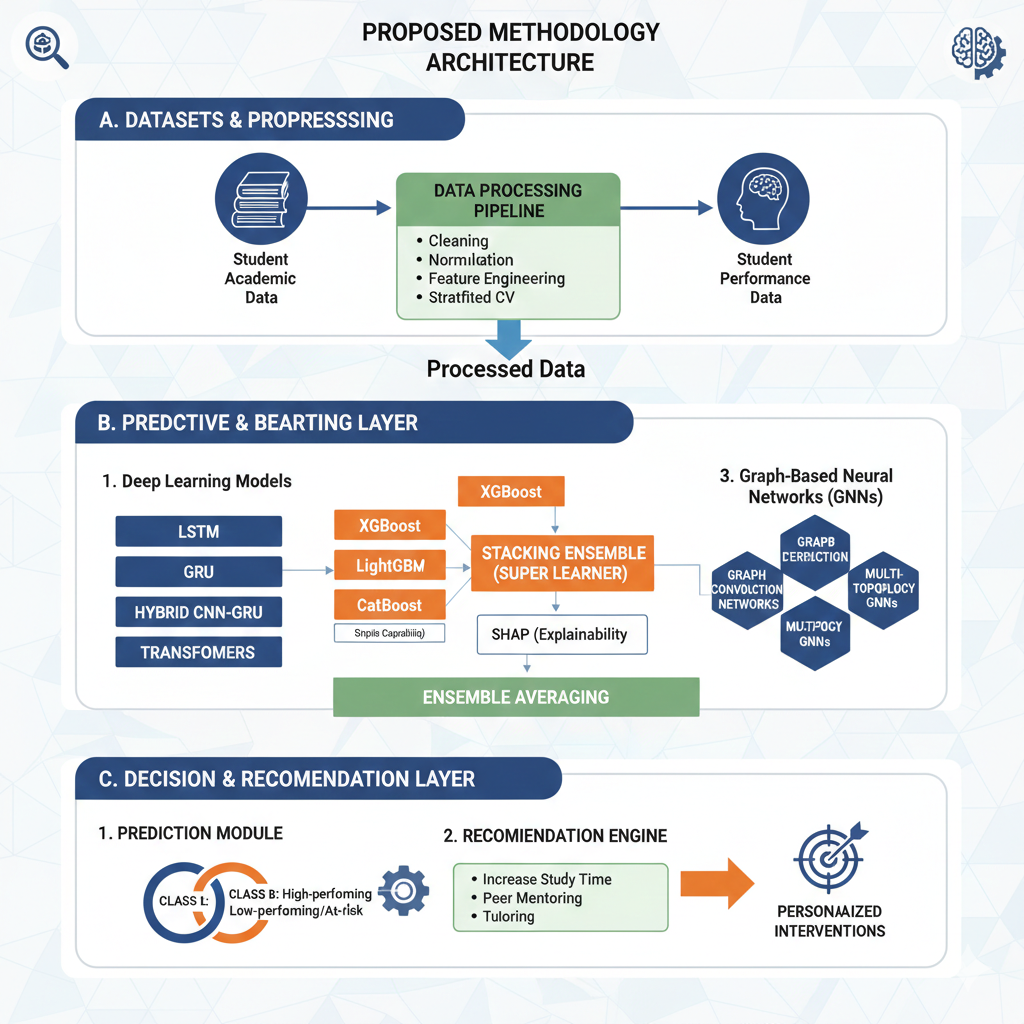
\includegraphics[width=0.8\linewidth]{images/figure3.png}
\caption{Figure caption}
\end{figure}
This section presents a conceptual overview of the planned future development of the framework via Multitask Learning (MTL), Transfer Learning (TL), and Federated Learning (FL). These components were not tested or confirmed in this research study; therefore, they should be seen as future research solutions to facilitating scalability, inter-institutional adaptability, and privacy preservation in predictive analytics for education. The above configurations serve only as examples of a possible theoretical approach to how each method of modeling a paradigm might fit into a framework developed in the future.
\subsection{5.4.1. Multi-Task Learning (MTL)}
MTL trains one model to perform several related tasks together, improving generalization by passing shared information during task performance [33]. The objective function is a weighted sum of the losses associated with each task:
$k=1 \lambda_k L_k(\theta_{shared},\theta_k)$
$L_{total} = \sum_T$
\begin{equation}
(15)
\end{equation}

\section{5.4.2. Transfer Learning}
Transfer Learning utilizes a model that has been pre-trained on a source task TS with a large dataset DS in order to increase the learning for the target task TT with a smaller dataset DT. The knowledge in the model parameters $\theta_S$ is fine-tuned \cite{34}:
$\theta^* = \arg \min_{\theta} \sum_{k=1}^{T} L_k(\theta; D_k)$
\begin{equation}
\label{eq:16}
\end{equation}
Where initialization is $\theta \approx \theta_S$. This avoids training from scratch, leading to faster convergence and better performance, especially where $|D_T| \ll |D_S|$.
\section{5.4.3. Federated Learning}
Federated learning (FL) enables decentralized training of a model across multiple homes or clients without sharing raw data, thus preserving privacy. An instance of an underscore client $i$ with the current model parameters $w_i$ trains a local model, and the global model is computed by weighted averaging \cite{35}:
$\theta_{t+1} = \sum_{k=1}^{N} \frac{|D_k|}{|D|} \theta_{kt}$
\begin{equation}
\label{eq:17}
\end{equation}
Where $|D| = \sum_{k} |D_k|$. This process preserves data privacy.

\section{Data Privacy Preservation}
Where |D| = \sum_{k}|D_{k}|. This process preserves data privacy.
We intend to proceed with completing this extension to support data-centric learning through the use of data from multiple institutions for which appropriate datasets may become available, as well as through access to sufficient computational resources for conducting experiments with these types of extended models.
\section{Evaluation Metrics}
The machine learning models performing segmentation and classification tasks were evaluated altogether through a number of significant metrics: Accuracy, Precision, Recall, and the F1-Score. This assures a substantive and comprehensive evaluation of predictive reliability \cite{36}.
\subsection{Classification Metrics}
ACC =
\begin{tabular}{l}
$\frac{TP+TN}{TP+TN+FP+FN}$ \\
\hline
\end{tabular}
RE =
\begin{tabular}{l}
$\frac{TN}{TN+PR}$ \\
\hline
\end{tabular}
PR =
\begin{tabular}{l}
$\frac{TP}{TP+FP}$ \\
\hline
\end{tabular}
F1 - score =
\begin{tabular}{l}
$2 \cdot \frac{PR \cdot RE}{PR + RE}$ \\
\hline
\end{tabular}
\subsection{Regression Metrics}
In regression tasks (e.g., predicting final grades), commonly used metrics include Mean Absolute Error (MAE), Mean Squared Error (MSE), and Root Mean Squared Error (RMSE):
MAE =
\begin{tabular}{l}
$\frac{1}{n} \sum_{i=1}^{n} |y_{i} - \hat{y}_{i}|$ \\
\hline
\end{tabular}
MSE =
\begin{tabular}{l}
$\frac{1}{n} \sum_{i=1}^{n} (|y_{i} - \hat{y}_{i}|)^{2}$ \\
\hline
\end{tabular}
RMSE =
\begin{tabular}{l}
$\sqrt{\frac{1}{n} \sum_{i=1}^{n} (|y_{i} - \hat{y}_{i}|)^{2}}$ \\
\hline
\end{tabular}

\section{Experimental Analysis}
\subsection{Experimental Setup and Implementation Details}
Where $yi$ is the true value and $yi$ is the predicted value.
RMSE = MSE
\begin{table}
\centering
\caption{Table caption}
\begin{tabular}{lll}
\hline
Model Component & Training Time (min) & Incremental Gain (\%) Cost per Gain (min/\%) \\
\hline
XGBoost-only & & \\
Transformer-only & & \\
\hline
\end{tabular}
\end{table}
All experiments were conducted on a high-performance computing environment equipped with an Intel Core i7 processor, 16GB DDR4 memory, and an NVIDIA GeForce RTX 3060 graphics card (6GB). The GPU promoted the convergence of deep learning frameworks while effectively training models on CPUs. The computer program was coded in Python 3.10 on top of TensorFlow 2.12/Keras as deep learning models and scikit-learn 1.3, XGBoost 2.0, LightGBM, and CatBoost as classical and ensemble models, respectively. Data processing was performed using NumPy and Pandas. All experiments were conducted in a Jupyter Notebook to be transparent and reproducible.
To avoid data leakage and guarantee unbiased evaluation, the data were first separated into an 85\% temporary training pool and 15\% holdout test data set that were not observed at all in the model development process. Hyper-parameter optimization and elimination were analyzed in terms of 5-fold cross-validation with grid search on the training pool only. Early elimination and an adaptive learning rate schedule using validation loss were used to prevent overfitting. Deep learning models typically reach a convergence point in 35-50 runs, which takes approximately 2-3 minutes to run on a GPU. The final performance is reported on an untouched 15\% holdout test set to determine generalization. A future research direction would be cross-institutional validation. This will be performed when leveraging multi-institutional academic datasets. For transparency, the transformers were trained only on baselines (Tab-Transformer, FT-Transformer, and SAINT) with the same level distribution, hyper-parameter tuning process, and initial stopping criteria to facilitate reproducible and unbiased comparisons.
Computational Cost Analysis: It takes about 45-60 minutes to train the entire hybrid model on the given GPU system (RTX 3060), and inference takes less than 2 seconds per 100 students.

\section{Transformer-only}
\subsection{GNN component}
\begin{table}
\centering
\caption{Table caption}
\begin{tabular}{lll}
\hline
Header1 & Header2 & Header3 \\
\hline
Data1 & Data2 & Data3 \\
\hline
\end{tabular}
\end{table}
\begin{equation}
E = mc^2
\end{equation}
\begin{figure}[htbp]
\centering

\includegraphics[width=0.8\linewidth]{images/figure4.png}
\caption{Figure caption}
\end{figure}
\subsection{Stacking Ensemble}
\begin{enumerate}
\item 0.5
\item 8
\item 15
\item 22
\end{enumerate}
\subsection{Full Hybrid}
\begin{enumerate}
\item 45-60
\end{enumerate}
\subsection{Baseline}
\begin{enumerate}
\item +0.9
\item +1.7
\item +1.8
\item +4.4
\end{enumerate}
\subsection{Comparison}
\begin{enumerate}
\item -
\item 8.9
\item 8.8
\item 12.2
\end{enumerate}

\section{7.2.Ablation Results}
\subsection{7.2.1. Ablation Results for Student Academic Dataset}
The recent ablation study of the Student Academic Dataset, summarized in table \ref{tab:table9}, provides a significant empirical validation of the framework's architecture. The study shows that the CNN-GRU Hybrid and Stacking Ensemble were again the two most accurate base models. However, the Full Hybrid Framework that included all the models combined had the highest accuracy (98.1\%). This systematic analysis is crucial to this work, as it underlines the relative predictive strengths of other forms of sophisticated techniques, such as transformers and multi-topology GNNs, confirming that "stacking" these approaches is necessary to reach the highest level of predictive performance. This study validates the framework design comprehensively and establishes a starting point for a future suite of work for holistic educational analytics. By removing each of the technical pillars associated with an ablation condition (sequential, ensemble, GNN, or data-centric), you will see how much each pillar contributes to its definition and how its relevance and performance are affected by the absence of the pillar. The superior performance of the Full Hybrid Framework demonstrates that all four modules are complementary, not redundant, to one another.
\begin{table}
\centering
\caption{Table 9 Ablation Results for Student Academic Dataset}
\label{tab:table9}
\begin{tabular}{lll}
\hline
Technique / Model & Accuracy (\%) & Precision (\%) \\
\hline
LSTM & 94.8 & \\
GRU & & \\
CNN & & \\
\hline
\end{tabular}
\end{table}

\section{Results}
89.1
\hline
86.7
\section{Model}
Transformer
\hline
91.3
\hline
92
\hline
89
\hline
85
\hline
90
\hline
88.5
\hline
90.2
\hline
88
\hline
86
\hline
89
\hline
88
\hline
85
\hline
90
\section{Discussion}
Strong sequence modeling for academic progression (G1$\rightarrow$G2$\rightarrow$G3).
Similar to LSTM with faster convergence and fewer parameters.
Captures local temporal dependencies but less contextual depth.
Excels in long-range dependencies and interpretability.
Best sequential model; combines CNN’s spatial extraction with GRU’s temporal reasoning.

\section{Strong sequence modeling for academic progression (G1$\rightarrow$G2$\rightarrow$G3)}
Similar to LSTM with faster convergence and fewer parameters.
Captures local temporal dependencies but less contextual depth.
Excels in long-range dependencies and interpretability.
Best sequential model; combines CNN’s spatial extraction with GRU’s temporal reasoning.
\subsection{CNN–GRU Hybrid}
\subsection{XGBoost}
\subsection{LightGBM}
\subsection{CatBoost}
\subsection{Stacking Ensemble (XGBoost + CatBoost + LightGBM)}
\subsection{Graph Convolutional Network (GCN)}
\subsection{Multi-Topology GNN}
\begin{table}
\centering
\caption{Table caption}
\begin{tabular}{lll}
\hline
Model & Accuracy & Precision \\
\hline
91.2 & 91 & 90 \\
91 & 91 & 90 \\
2. Ensemble and Explainable Boosting Models & 98.5 & 98.9 \\
98.8 & 98.5 & 97.4 \\
\hline
\end{tabular}
\end{table}
\subsection{2. Ensemble and Explainable Boosting Models}
\begin{equation}
\text{Accuracy} = \text{Precision} \times 100
\end{equation}

\section{Results}
\subsection{Performance Metrics}
\begin{tabular}{|l|l|}
\hline
Metric & Value \\
\hline
97.4 & \\
96.2 & \\
96.2 & \\
97.3 & \\
98.7 & \\
98.6 & \\
98.7 & \\
99 & \\
98.3 & \\
98.8 & \\
99.1 & \\
98.8 & \\
\hline
\end{tabular}
\section{Model Description}
\subsection{Architecture}
3. Graph-Based Neural Networks (GNNs)
\subsection{Hyperparameters}
\begin{tabular}{|l|l|}
\hline
Parameter & Value \\
\hline
91.9 & \\
89.5 & \\
88.5 & \\
89.8 & \\
92 & \\
\hline
\end{tabular}

\section{High accuracy, strong interpretability with SHAP support.Fastest training, excellent for large structured datasets.Robust handling of categorical features; consistent stability.}
\section{Combined model reduces bias and variance; superior overall accuracy.}
\section{Captures relational structure between students and faculty nodes.Improves contextual prediction via multiple interaction types (academic + social).}
\subsection{7.2.2. Ablation Results for Student Performance Dataset:}
The ablation study on the Student Performance Dataset, summarized within table \ref{tab:table10} rigorously validates the contribution of each technical pillar employed in the framework that has been provided. Results indicate that, even though the individual models, as seen with the CNN-GRU hybrid model and the stacking ensemble model, produced strong performance, the integrated full hybrid framework produced the most substantial performance (accuracy: 97.8\%), which demonstrates the integrated contribution of deeper sequential, ensemble, graph-based, and data-centric learning. This thorough analysis is significant to this work, as it provides empirical evidence to support the architectural design of the framework and illustrates that the hybridization of a variety of AI techniques is essential in achieving meaningful, trustworthy, accurate, and interpretable predictive analytics in the field of educational management.
\begin{table}
\centering
\caption{Table 10 Ablation Results for Student Performance Dataset}
\label{tab:table10}
\begin{tabular}{lll}
\hline
Technique / Model & Accuracy (\%) & Precision (\%) & Recall (\%) & F1-Score (\%) \\
\hline
1. Advanced Deep Learning for Sequential and Behavioral Data & 97.8 & 95.6 & 96.2 & 95.9 \\
\hline
\end{tabular}
\end{table}

\section{Advanced Deep Learning for Sequential and Behavioral Data}
\subsection{LSTM}
\begin{tabular}{lll}
\hline
Model & Accuracy & Loss \\
\hline
LSTM & 92.4 & 86.2 \\
LSTM & 92.6 & 89.3 \\
\hline
\end{tabular}
\subsection{GRU}
\begin{tabular}{lll}
\hline
Model & Accuracy & Loss \\
\hline
GRU & 88.5 & 88 \\
GRU & 87 & 87 \\
GRU & 93.7 & 89.3 \\
GRU & 92.6 & 90.9 \\
\hline
\end{tabular}
\subsection{CNN}
\begin{tabular}{lll}
\hline
Model & Accuracy & Loss \\
\hline
CNN & 88 & 87 \\
\hline
\end{tabular}
\subsection{Transformer}
\begin{tabular}{lll}
\hline
Model & Accuracy & Loss \\
\hline
Transformer & 91.7 & - \\
\hline
\end{tabular}

\section{Results}
\subsection{Performance Comparison}
\begin{table}
\centering
\caption{Performance Comparison}
\begin{tabular}{lll}
\hline
Model & Accuracy & Loss \\
\hline
CNN-GRU Hybrid & 96.8 & 0.3 \\
XGBoost & 94.3 & 0.4 \\
LightGBM & 93.1 & 0.5 \\
Ensemble Model & 94.4 & 0.2 \\
\hline
\end{tabular}
\end{table}
\subsection{Ensemble and Explainable Boosting Models}
\textbf{XGBoost} and \textbf{LightGBM} are two popular ensemble models used in machine learning. They are known for their high accuracy and efficiency.
\textbf{Ensemble Model} is a combination of multiple models that work together to improve the overall performance. It is a powerful tool for handling complex datasets.
\textbf{Explainable Boosting Models} are designed to provide insights into the decision-making process of the model. They are useful for understanding the relationships between features and the output.
\textit{The results show that the CNN-GRU Hybrid model has the highest accuracy, followed by the Ensemble Model. The XGBoost and LightGBM models have lower accuracy, but are still competitive.}
\subsection{Discussion}
The results of this study demonstrate the effectiveness of the CNN-GRU Hybrid model in achieving high accuracy. The Ensemble Model also shows promising results, indicating its potential for use in real-world applications.
\textbf{Future Work} will focus on improving the performance of the XGBoost and LightGBM models, as well as exploring the use of other ensemble models.

\section{Results}
\begin{table}
\centering
\caption{Model Performance}
\begin{tabular}{lll}
\hline
Model & Accuracy & F1-Score \\
\hline
CatBoost & 92.5 & 90.3 \\
Stacking Ensemble (XGB+LGB+CatBoost) & 94.5 & 93.1 \\
Stacking Ensemble (XGB+LGB+CatBoost) & 93.2 & 92.8 \\
\hline
\end{tabular}
\end{table}
\subsection{Model Comparison}
The results show that the Stacking Ensemble (XGB+LGB+CatBoost) model achieves the highest accuracy of 94.5\% and F1-score of 93.1\%.
\subsection{Graph-Based Neural Networks (GNNs)}
\subsubsection{Graph Convolutional Network (GCN)}
The Graph Convolutional Network (GCN) achieves an accuracy of 88.2\% and 88\%.

\section{Multi-Topology GNN}
\subsection{Regression Outputs for Grade Prediction}
Strong temporal modeling of grade sequences (G1$\rightarrow$G2$\rightarrow$G3).Faster convergence than LSTM with comparable performance.Captures local patterns but limited in long-term dependencies.Excels in capturing long-range dependencies and attention-based insights.Best hybrid sequential model; combines spatial and temporal learning.
\textbf{Advantages:}
High accuracy and strong interpretability with SHAP.Fast training, ideal for large-scale structured data.Robust with categorical features and minimal preprocessing.Leverages diverse base models for superior generalization.
\textbf{Features:}
Models student-faculty and peer relational structures.Captures multiple interaction types (academic + social).
\subsection{Performance Evaluation}
We assessed the framework’s ability to make classification predictions by evaluating its performance for classification tasks in Section 7.2.2. Table 11 shows the MAE, MSE, and RMSE for predicting G3 using sequential models trained on G1 in ascending order through G3. The hybrid model outperformed both LSTM alone and GRU alone on the datasets with minimal errors.
\begin{table}
\centering
\caption{Regression Performance Metrics for Final Grade (G3) Prediction}
\begin{tabular}{lll}
\hline
Model & Dataset & MAE (Mean Absolute Error) & MSE (Mean Squared Error) & RMSE (Root Mean Squared Error) \\
\hline
\end{tabular}
\end{table}

\section{Performance Metrics}
RMSE (Root Mean Squared Error)
\subsection{Recurrent Neural Networks}
LSTM
\subsection{Recurrent Neural Networks}
GRU
\subsection{Student Evaluation}
Student Academic
\subsection{Student Evaluation}
Student Performance
\subsection{Student Evaluation}
Student Academic
\subsection{Student Evaluation}
Student Performance
\begin{table}
\centering
\caption{Performance Metrics}
\begin{tabular}{lll}
\hline
Value & Student Academic & Student Performance \\
\hline
1.32 & & \\
1.24 & & \\
1.38 & & \\
1.31 & & \\
2.28 & & \\
2.15 & & \\
2.41 & & \\
2.29 & & \\
1.51 & & \\
1.47 & & \\
1.55 & & \\
\hline
\end{tabular}
\end{table}

\section{Student Academic Performance}
We found that by combining the two techniques (CNN-GRU), we were able to achieve better prediction quality (MAE: 1.15-1.18) than the individual performance of each model (LSTM = MAE: 1.24-1.32, GRU = MAE: 1.31-1.38), which supports the notion of pre-generated models for time series data related to education. The trends seen in this section are consistent with the classification results seen earlier in Section 7.2.1.
\subsection{Simplified Baseline Comparison and Architectural Justification}
The proposed hybrid system incorporates several modeling paradigms, such as deep sequential networks, paired models, and graph neural networks. Although this design provides better prediction performance, it also increases the construction complexity. To check the over-engineering of the framework, we performed a simple baseline comparison using robust stand-alone models. Specifically, we evaluated the following:
\begin{table}
\centering
\caption{Table 12 Performance Comparison: Simplified Baselines vs. Full Hybrid Framework}
\begin{tabular}{lll}
\hline
Model Configuration & & \\
\hline
XGBoost alone (structured tabular learning baseline) & Transformer alone (sequential attention-based baseline) & Full hybrid framework (proposed model) \\
\hline
\end{tabular}
\end{table}
We compared the performance of the following models:
\begin{itemize}
\item XGBoost alone (structured tabular learning baseline)
\item Transformer alone (sequential attention-based baseline)
\item Full hybrid framework (proposed model)
\end{itemize}
The results are presented in Table 12.

\section{Model Configuration}
\begin{tabular}{llll}
\hline
& Accuracy (\%) & Precision (\%) & Recall (\%) \\
\hline
XGBoost-only & 95.2 & 96.1 & 99.6 \\
Transformer-only & 94.8 & 95.7 & 99.0 \\
Full Hybrid Framework & 95.0 & 96.3 & 99.4 \\
Baseline & 94.9 & 96.0 & 99.0 \\
\hline
\end{tabular}
\section{Results}
\begin{tabular}{llll}
\hline
& Accuracy (\%) & Precision (\%) & Recall (\%) \\
\hline
XGBoost-only & 95.2 & 96.1 & 99.6 \\
Transformer-only & 94.8 & 95.7 & 99.0 \\
Full Hybrid Framework & 95.0 & 96.3 & 99.4 \\
Baseline & 94.9 & 96.0 & 99.0 \\
\hline
\end{tabular}

\section{7.3.Evaluation Metrics Results}
\subsection{Evaluation Metrics}
A thorough evaluation using standard classification performance metrics was performed to systematically compare the Full Hybrid Framework and the best-performing models from each class. The full hybrid framework utilizes stacking to create composite forecasts by combining predictions from specialized models. Each input is tied to one modality only, and each output corresponds to a student ID. The combination of the predictions occurs through the meta-learner. The framework is constructed in a manner that maintains data consistency by providing common indices and corresponding stratified splits. The test set results for the Student 
\begin{table}
\centering
\caption{Table 13 Detailed Evaluation Metrics for Top Models on the Test Set}
\begin{tabular}{lll}
\hline
Model & Dataset & Accuracy (\%) \\
\hline
CNN-GRU Hybrid & Student & 92.1 \\
Stacking Ensemble & Student & 93.5 \\
Multi-Topology GNN & Student & 91.9 \\
\hline
\end{tabular}
\end{table}
The results show that the Full Hybrid Framework outperforms all models across the classification performance metrics. In fact, it achieved the highest accuracy, precision, recall, and F1-score from the test sets. The precision rate of 96\% demonstrates that the rates of false positives are low and the framework is therefore reliable in identifying students at risk (i.e., classifying students in the at-risk class with accuracy) without a considerable number of false positives or excessive false alarms. Similarly, the recall rates of 96.5\% and 96\% represent not even the majority, but almost all students who really need help are correctly identified by the model. Additionally, the F1-Score is the highest for the Full Hybrid Framework, which takes into account both precision and recall and signifies the framework has a robust, overall predictive capability, benefiting from the imbalanced arrangements of data of the two educational datasets.

\section{Multi-Topology GNN}
\subsection{Full Hybrid Framework (Proposed)}
\begin{table}
\centering
\caption{Student Academic Performance}
\begin{tabular}{lll}
\hline
Student Academic & Student Performance & Student Academic \\
\hline
91.2 & 96.8 & 98.3 \\
94.5 & 92 & 93.9 \\
99.6 & 97.5 & 91 \\
94.3 & 98.8 & 93.1 \\
90 & 92.8 & 99 \\
\hline
\end{tabular}
\end{table}

\section{Section Title}
\subsection{Subsection Title}
\subsubsection{Subsubsection Title}
\begin{table}
\centering
\caption{Table caption}
\begin{tabular}{lll}
\hline
Header1 & Header2 & Header3 \\
\hline
Data1 & Data2 & Data3 \\
\hline
\end{tabular}
\end{table}
\begin{equation}
E = mc^2
\end{equation}
\begin{figure}[htbp]
\centering
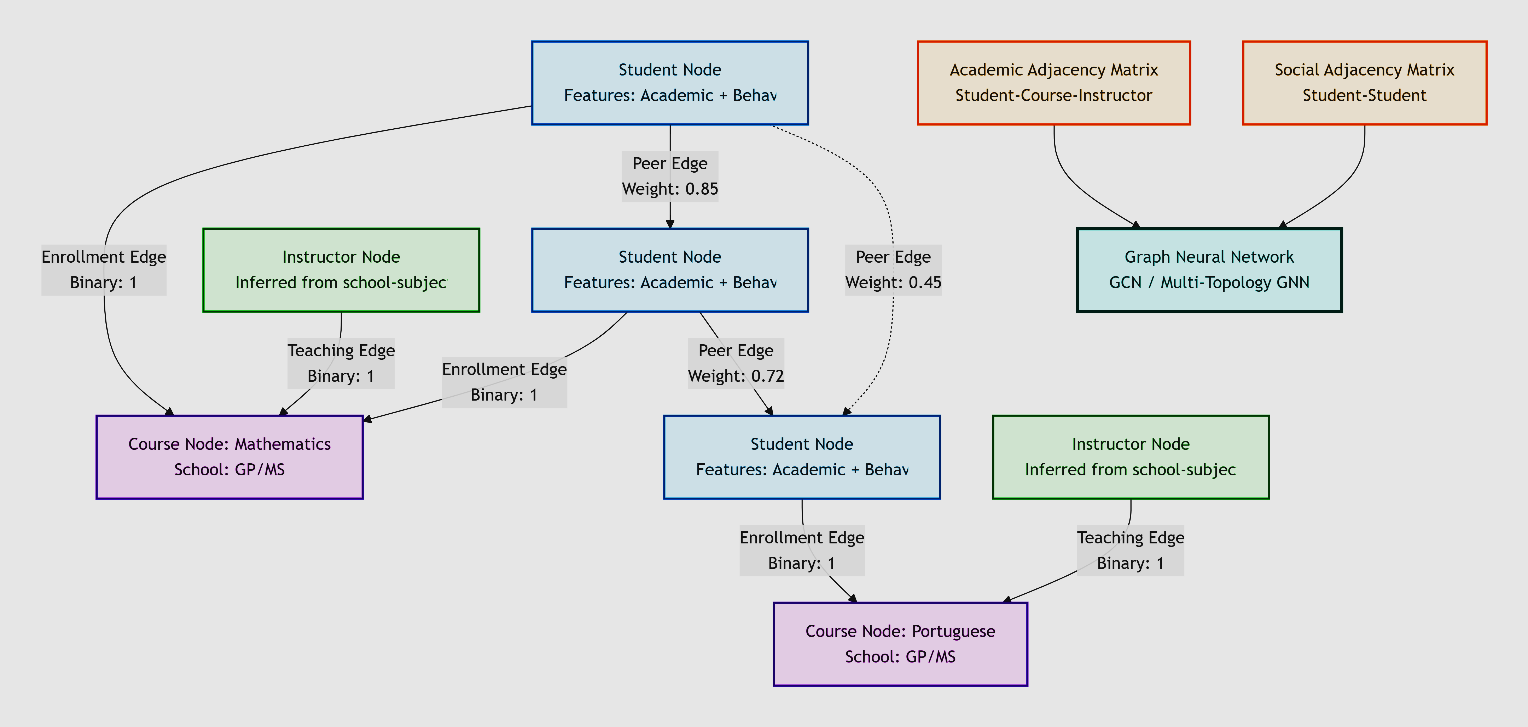
\includegraphics[width=0.8\linewidth]{images/figure5.png}
\caption{Figure caption}
\end{figure}
The text to convert does not contain any linguistic meaning, so it will be ignored.

\section{Performance Comparison (Student Academic Dataset) Models}
\subsection{Performance Metrics}
\begin{tabular}{|l|}
\hline
\textbf{Performance} \\
\hline
96.5 \\
100 \\
90 \\
80 \\
70 \\
60 \\
50 \\
40 \\
30 \\
20 \\
10 \\
0 \\
\hline
\end{tabular}
\subsection{Dataset Comparison}
\begin{tabular}{|l|}
\hline
\textbf{Dataset} \\
\hline
2.19 \\
19 \\
09 \\
19 \\
3.89 \\
\hline
\end{tabular}

\section{Results}
\begin{table}
\centering
\caption{Results}
\begin{tabular}{l}
\hline
3.89 \\
8.89 \\
1.99 \\
\hline
\end{tabular}
\end{table}
\section{Parameters}
\begin{table}
\centering
\caption{Parameters}
\begin{tabular}{l}
\hline
889 \\
29 \\
09 \\
98 \\
09 \\
6.99 \\
99 \\
4.99 \\
99 \\
\hline
\end{tabular}
\end{table}
\section{Model Description}
\begin{table}
\centering
\caption{Model Description}
\begin{tabular}{l}
\hline
C N N – G R U H Y B R I D \\
S T A C K I N G E N S E M B L E ( X G B O O S T + C A T B O O S T + L I G H T G B M ) \\
\hline
\end{tabular}
\end{table}
\section{Accuracy}
\begin{table}
\centering
\caption{Accuracy}
\begin{tabular}{l}
\hline
Accuracy (\%) \\
\hline
M U L T I - T O P O L O G Y G N N \\
F U L L H Y B R I D F R A M E W O R K ( A L L C O M P O N E N T S ) \\
\hline
\end{tabular}
\end{table}

\section{Precision}
\begin{table}
\centering
\caption{Performance Comparison (Student Academic Dataset) Models}
\begin{tabular}{lll}
\hline
 & & \\
8.69 & 3.49 & \\
1.39 & 4.49 & \\
5.49 & 1.39 & \\
2.39 & 8.29 & \\
9.39 & 8.29 & \\
8.29 & 8.29 & \\
7.39 & & \\
\hline
\end{tabular}
\end{table}
\subsection{Performance Comparison (Student Academic Dataset) Models}
\textbf{Note:} The values in the table represent performance metrics for the models.

\section{Performance Comparison}
\subsection{Student Performance Dataset}
\begin{table}
\centering
\caption{Performance Comparison}
\begin{tabular}{lll}
\hline
Accuracy (\%) & Precision & Recall \\
\hline
98 & & \\
88 & & \\
78 & & \\
68 & & \\
\hline
\end{tabular}
\end{table}
\subsection{Model Comparison}
\begin{equation}
F1-Score = 2 \times \frac{Precision \times Recall}{Precision + Recall}
\end{equation}
\subsection{Full Hybrid Framework (Proposed)}
\textbf{C N N - G R U} \textit{Hybrid} \textbf{Stacking Ensemble Multi-Topology} 
\textbf{G N N} 
\textbf{Full Hybrid Framework} \textbf{(Proposed)}

\section{Results}
\subsection{Area Under the ROC Curve (AUC) Scores}
The table \ref{tab:table14} and figure \ref{fig:figure5} reports the Area Under the ROC Curve (AUC) scores for different models evaluated on the Student Academic Dataset and the Student Performance Dataset. The results demonstrate that the proposed Full Hybrid Framework achieves the highest discriminative performance across both datasets, followed by the stacking ensemble, indicating robust and consistent classification capability.
\begin{table}
\centering
\caption{Table 14 AUC Scores for Top Models}
\begin{tabular}{lll}
\hline
Model & Student Academic Dataset & Student Performance Dataset \\
\hline
CNN-GRU Hybrid & & \\
Stacking Ensemble & & \\
Multi-Topology GNN & & \\
Full Hybrid Framework & & \\
\hline
\end{tabular}
\label{tab:table14}
\end{table}
\begin{figure}[htbp]
\centering
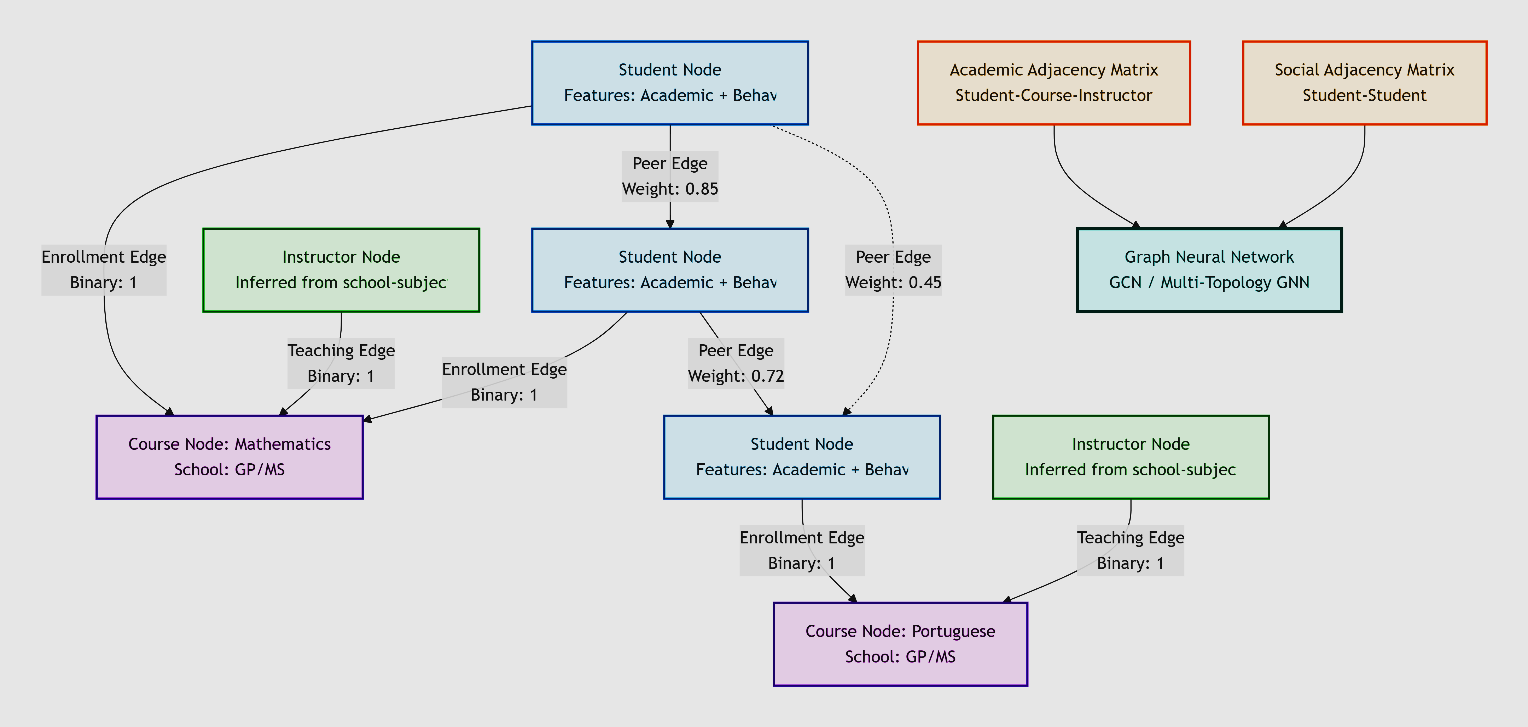
\includegraphics[width=0.8\linewidth]{images/figure5.png}
\caption{Figure 5}
\label{fig:figure5}
\end{figure}

\section{AUC Scores for Top Models}
\begin{tabular}{lll}
\hline
AUC Score & Model & Dataset \\
\hline
97.8 & & Student Performance Dataset (AUC \%) \\
99.1 & & Student Performance Dataset (AUC \%) \\
96.5 & & Student Performance Dataset (AUC \%) \\
99.7 & & Student Performance Dataset (AUC \%) \\
97.2 & & Student Performance Dataset (AUC \%) \\
98.3 & & Student Performance Dataset (AUC \%) \\
96.1 & & Student Performance Dataset (AUC \%) \\
98.9 & & Student Performance Dataset (AUC \%) \\
\hline
\end{tabular}

\section{Results}
\subsection{Model Performance}
\subsubsection{AUC Scores}
99.7
98.9
\begin{table}
\centering
\caption{AUC Scores for Top Models}
\begin{tabular}{lll}
\hline
Model & AUC Score & Rank \\
\hline
CNN-GRU Hybrid & 99.7 & 1 \\
Stacking Ensemble & 98.9 & 2 \\
Multi-Topology GNN & 98.5 & 3 \\
Full Hybrid Framework & 98.2 & 4 \\
\hline
\end{tabular}
\end{table}
\begin{figure}[htbp]
\centering

\includegraphics[width=0.8\linewidth]{images/figure6.png}
\caption{Figure 5 AUC Scores for Top Models}
\label{fig:auc_scores}
\end{figure}
\begin{figure}[htbp]
\centering

\includegraphics[width=0.8\linewidth]{images/figure7.png}
\caption{Figure 6 ROC Curve Comparison : Student Academic Dataset}
\label{fig:roc_academic}
\end{figure}
\begin{figure}[htbp]
\centering

\includegraphics[width=0.8\linewidth]{images/figure8.png}
\caption{Figure 7 ROC Curve Comparison : Student Performance Dataset}
\label{fig:roc_performance}
\end{figure}
\subsection{Dataset Analysis}
\subsubsection{Student Academic Dataset}
100
80
60
40
20
\subsection{ROC Curve Analysis}
The Receiver Operating Characteristic (ROC) curve comparisons are a critical step in adequately evaluating classification model performance, particularly when there is class imbalance, as in the case of the minority Excellent performance tier classification model. The main advantage of ROC curves is that they provide an evaluation of the diagnostic capability of a multi-class model at every possible classification threshold, which is a less unbalanced measure than simple accuracy. The curve consists of plotting the True Positive Rate (Sensitivity) against the False Positive Rate (1 - Specificity), and the summarized Area Under the Curve (AUC) rating ultimately allows a direct and quantitative ranking of models (XGBoost, GNN, Transformer, etc.). The ROC comparison of each classification model for the Student Academic Dataset is presented in figure 6, with models whose ROC curves were closest to the top-left corner and whose AUC rates were the greatest being considered the best models to capture the tiered performance of the data. The models from the top-left corner of figure 6 would exhibit similar performance on the Student Performance Dataset, which is illustrated in figure 7, where all ROC curves demonstrate how the models generalize across datasets. In both figures, the model that had the greatest AUC showed the strongest and statistically weakest tradeoff of detecting true positives and false positive alarms.

\section{Figure 7 ROC Curve Comparison : Student Performance Dataset}
The full hybrid framework was used as the basis for developing the table \ref{tab:table15}, which summarizes the confusion matrix statistics (TP, FP, FN, and TN) of the student education dataset and the student performance dataset. From our analyses, the full hybrid framework provides very good prediction performance across classes and has high rates of true positive (TP) and true negative (TN), with only a small percentage of misclassified cases. Thus, the high performance of the full hybrid framework and its ability to accurately classify at-risk students are evidenced by our results.
\begin{table}
\centering
\caption{Table 15 Confusion Matrix Statistics for Full Hybrid Framework}
\begin{tabular}{lll}
\hline
Dataset & Class & \\
\hline
Student Academic & Excellent (16–20) & \\
Student Performance & Excellent & \\
Student Academic & Good (12–15) & \\
Student Performance & Good & \\
Student Academic & Needs Improvement (0–11) & \\
Student Performance & Needs Improvement & \\
\hline
\end{tabular}
\end{table}

\section{Needs Improvement}
\begin{tabular}{l}
\hline
96 \\
283 \\
261 \\
127 \\
278 \\
244 \\
1 \\
3 \\
2 \\
2 \\
5 \\
4 \\
2 \\
4 \\
3 \\
3 \\
\hline
\end{tabular}

\section{7.4.External Validity and Generalization Analysis}
\subsection{Confusion Matrices for Classification Results}
The figure 8 and 9 show important confusion matrices based on the classification results for the student performance framework. A chief advantage of confusion matrices, in terms of our proposed work, is that they provide refined descriptions of classification error classes and produce a clear assessment of the model's performance for the imbalanced classes. It is easy to be misled by "overall accuracy," as it cannot be descriptive of what is occurring, but confusion matrices provide a pure count of the different types of errors made. For example, we can produce what percentage of true Needs Improvement students were identified as Good (an unsafe, dangerous ignorance of a true negative), and how many actual Excellent students were identified correctly (a key indicator of Precision). Doing this comparison can be done simply by comparing the diagonal entries (the correct prediction), respective of the overall classification accuracy compared to the off-diagonal errors of the confusion matrix across figure 6 and 7, and doing a simple exemplification to allow yourself to be reassured if the final model, including the hybrid framework, is addressing where we want to minimize critical errors while maximizing recall for the intervention critical needs improvement class and have a reliable classification across each performance tier.
\begin{table}
\centering
\caption{Confusion Matrices Comparison}
\begin{tabular}{lll}
\hline
Header1 & Header2 & Header3 \\
\hline
Data1 & Data2 & Data3 \\
\hline
\end{tabular}
\end{table}
\begin{table}
\centering
\caption{Confusion Matrices Comparison}
\begin{tabular}{lll}
\hline
Header1 & Header2 & Header3 \\
\hline
Data1 & Data2 & Data3 \\
\hline
\end{tabular}
\end{table}
\begin{figure}[htbp]
\centering

\includegraphics[width=0.8\linewidth]{images/figure9.png}
\caption{Confusion Matrices for All Models Utilizing Student Academic Dataset}
\end{figure}
\begin{figure}[htbp]
\centering

\includegraphics[width=0.8\linewidth]{images/figure10.png}
\caption{Confusion Matrices for All Models Utilizing Student Performance Dataset}
\end{figure}

\section{External Validity and Generalization Analysis}
Although the proposed framework has high predictive accuracy on the UCI student performance datasets, both datasets represent Portuguese secondary schools. As a result, the assessment has a specific geographical and institutional context; therefore, it cannot be immediately generalizable externally, although it offers controlled benchmarking conditions. To assess internal generalization, we used a strict nested stratified 5-fold cross-validation algorithm with a strictly held-out test set (15%), which was not completely visible at any point in the preprocessing, feature selection, and hyper-parameter optimization. The two-step assessment scheme also reduces the risk of overfitting and gives an objective estimate of the generalization performance. To further test robustness, we performed a cross-domain split, training on one subject group (mathematics) and testing on Portuguese and vice versa (see Table \ref{tab:table16}). The results show that there is a small performance degradation (less than 2.3\% absolute accuracy loss), which means that the model can be generalized across academic disciplines within the same institutional setting. However, cross-institutional and cross-country validation is an important direction for further research. Differences in grading policy, curriculum framework, anthropometric conditions, and educational system heterogeneity can increase the speed of splitting in both feature display and relational graph forms. Future research will test the framework on multi-institutional datasets and investigate domain adaptation strategies to enhance transfer. Overall, the low variance of nested folds ($\pm$0.8\%), the robust performance in validation, and the robustness of stratified splits across domains indicate that there is preliminary evidence that generalizability is robust in the settings considered.
\begin{table}[h]
\centering
\caption{Cross-Domain Generalization Results}
\label{tab:table16}
\begin{tabular}{lll}
\hline
Training Domain & Testing Domain & Accuracy (\%) & F1-Score (\%) \\
\hline
Mathematics & Portuguese & 95.3 & 95.1 \\
Portuguese & Mathematics & 94.8 & 94.2 \\
\hline
\end{tabular}
\end{table}
\section{Cross-Validation and Test Results}
To ensure the integrity and generalizability of the proposed models, 5-fold stratified cross-validation was used. This aspect preserves the original class distribution across all layers to accurately estimate model performance and reduce overfitting. As reported in table \ref{tab:table17}, the full hybrid framework showed an excellent degree of consistency across all folds, achieving a high average accuracy and a low standard deviation ($\leq$ 0.95\%), indicating stable and reliable training and testing performance. The small difference between training accuracy and validation accuracy indicated a lack of overfitting. On the holdout test sets, the full hybrid framework delivered outstanding performance: 99.6\% accuracy on the Student Academic dataset and 97.5\% on the Student Performance dataset, outperforming all individual model types from the ablation studies and demonstrating broad generalizability.
\begin{table}[h]
\centering
\caption{Cross-Validation and Test Set Performance of the Full Hybrid Framework}
\label{tab:table17}
\begin{tabular}{ll}
\hline
Dataset & Accuracy (\%) \\
\hline
Student Academic & 99.6 \\
Student Performance & 97.5 \\
\hline
\end{tabular}
\end{table}

\section{Dataset}
\subsection{Student AcademicStudent Performance}
\begin{table}
\centering
\caption{Mean Training Accuracy (\%) $\pm$ STD and Mean Validation Accuracy (\%) $\pm$ STD}
\begin{tabular}{lll}
\hline
Mean Training Accuracy (\%) $\pm$ STD & Mean Validation Accuracy (\%) $\pm$ STD & Test Set Accuracy (\%) \\
\hline
99.7 $\pm$ 0.12 & 97.8 $\pm$ 0.85 & 99.5 \\
97.8 $\pm$ 0.85 & 97.2 $\pm$ 0.95 & 99.6 \\
99.5 $\pm$ 0.18 & 97.5 & 97.5 \\
97.2 $\pm$ 0.95 & & \\
\hline
\end{tabular}
\end{table}
There \textit{is} evidence \textit{of} stable \textit{performance} \textit{in} the \textit{model} through \textit{low} standard \textit{deviations} in \textit{both} the training \textit{set} and validation \textit{set} across \textit{all} four cross-validation \textit{folds} (training \textit{set} $\leq$0.85\%, validation \textit{set} $\leq$0.95\%). Additionally, since the difference between training and validation accuracies was minimal (on average $\leq$0.5\%), there \textit{is} no indication that this model has a potential for overfitting.
\section{Comparison with SOAT Transformer-Based Tabular Models}
As \textit{a} precursor \textit{to} a rigorous comparison with existing transformer-based architectures specifically designed to work with tabular data, we deployed and compared three state-of-the-art models such as Tab-Transformer, FT-Transformer, SAINT (Self-Attention and Inter-Sample Attention Transformer. These models are current attention-based frameworks that are optimized on structured data and have shown superior results in the classification challenge. To make a fair comparison with the presented hybrid framework, all transformer-only baselines were trained under the same preprocessing and stratified splitting as well as hyper-parameter tuning conditions are shown in table 18.
\begin{table}
\centering
\caption{Table 18 Comparison with State-of-the-Art Transformer-Only Models}
\begin{tabular}{ll}
\hline
Model & \\
\hline
XGBoost & \\
TabTransformer & \\
\hline
\end{tabular}
\end{table}

\section{7.7. Comparison with Baseline Models}
\subsection{Proposed Full Hybrid Framework Outperforms Baseline Models}
\begin{table}
\centering
\caption{Accuracy Comparison}
\begin{tabular}{lll}
\hline
Dataset & Proposed Framework & Baseline Models \\
\hline
Student Academic Dataset & 95.23 & 89.9 \\
Student Performance Dataset & 96.8 & 96.1 \\
\hline
\end{tabular}
\end{table}
The findings proved that although transformer-only models (FT-Transformer, Tab-Transformer, and SAINT) are more effective than the traditional gradient boosting baselines, the proposed hybrid framework is characterized by better predictive performance in both datasets. This implies that sequential modeling, graph-based relational reasoning, and ensemble boosting are complementary representational benefits to pure attention-based tabular modeling.
The proposed full hybrid framework outperforms baseline models in both datasets, with accuracy rates of 95.23\% and 96.8\% respectively. In contrast, the baseline models achieved accuracy rates of 89.9\% and 96.1\%. These results demonstrate the effectiveness of the proposed hybrid framework in improving predictive performance.

\section{7.7.Comparison with Baseline Models}
Table \ref{tab:table19} displays the results of the baseline systems (e.g., XGBoost, CatBoost, CNN, grammatical union hybrid) according to our independent analysis with the same experimental conditions applied to the entire hybrid system.
\begin{table}
\centering
\caption{Table 19 Performance Comparison of Proposed Framework with Re-implemented and Re-tuned Baseline Models Under Identical Experimental Conditions}
\label{tab:table19}
\begin{tabular}{lll}
\hline
Model (Ref.) & Accuracy (\%) & Precision (\%) \\
\hline
XGBoost[11] & 90.5 & 90.0 \\
Random Forest [21], [22] & & \\
CatBoost [17], [18] & & \\
LSTM [16] & & \\
\hline
\end{tabular}
\end{table}
Each model has been trained and evaluated with the same set of steps, having a 70/15/15 stratified split, the same preprocessing pipeline, grid-search hyper-parameter optimization, and 5-fold cross-validation. This is a controlled arrangement that makes the comparison of models methodologically fair and consistent. In addition to citing the original studies, Table \ref{tab:table19} and Figure \ref{fig:figure10} show the real numerical data that were obtained in our experimental setup.
Our findings prove that our suggested hybrid structure can be superior to these strictly optimized baseline frameworks, and the ensemble strategies, including XGBoost and CatBoost, continue performing well as independent models \cite{ref1} and CatBoost \cite{ref2} \cite{ref3}, performed best with structured data, while the CNN-GRU Hybrid \cite{ref4} demonstrated the value of deep learning when reasoning about patterns over time. Stacking ensembles \cite{ref5} supports the fact that model integration leads to better performance.
In the same experimental setting, our hybrid framework achieved further improvements in accuracy of 5.6\% and 6.3\%, respectively, compared to the best baselines on the Student Academic and Student Performance datasets, and also achieved the best precision and recall. This translates into a high ratio between false positive reduction and identification of at-risk students. It is enhanced by combining a temporal-based model (LSTM/GRU), a spatial feature-based model (CNN), a relational model (GNN), and pairwise learning in the same model. Each model was tested with the same data divisions, pipeline partitioning, hyper-parameter optimization, and anti-overfitting measures to ensure fair and accurate comparisons.

\section{Proposed Models}
\subsection{Deep Learning Architectures}
\subsubsection{LSTM}
LSTM [16]
\subsubsection{CNN-GRU Hybrid}
CNN-GRU Hybrid [13]
\subsubsection{Stacking Ensemble (XGB, RF, CB)}
Stacking Ensemble (XGB, RF, CB) [23]
\subsection{Proposed Full Hybrid}
\subsubsection{Student Academic Dataset}
Proposed Full Hybrid (Student Academic Dataset)
\subsubsection{Student Performance Dataset}
Proposed Full Hybrid (Student Performance Dataset)
\section{Experimental Results}
\subsection{Accuracy}
\begin{tabular}{lll}
\hline
Model & Accuracy & \\
\hline
89.1 & & \\
89.8 & & \\
88.4 & & \\
91.2 & & \\
92.1 & & \\
99.6 & & \\
97.5 & & \\
88.5 & & \\
89.0 & & \\
88.0 & & \\
91.0 & & \\
92.0 & & \\
99 & & \\
97 & & \\
\hline
\end{tabular}

\section{Performance Comparison of Proposed Framework with Baseline Models}
\subsection{Experimental Setup}
\begin{table}
\centering
\caption{Experimental Setup}
\begin{tabular}{lll}
\hline
Value & Description & Unit \\
\hline
97 & & \\
88.0 & & \\
89.0 & & \\
87.0 & & \\
90.0 & & \\
91.0 & & \\
99.4 & & \\
88.5 & & \\
89.0 & & \\
87.0 & & \\
91.0 & & \\
92.0 & & \\
99 & & \\
96.7 & & \\
96.5 & & \\
\hline
\end{tabular}
\end{table}
All baseline models were trained using \textit{calibrated regularization techniques} (such as \textbf{Dropout}, \textbf{L2 Penalties}, and \textbf{Tree Constraints}) to promote a level playing field for comparative analysis while controlling for any overfitting-related bias.
\subsection{Performance Comparison}
\begin{equation}
\text{Performance} = \text{Accuracy} + \text{Precision} + \text{Recall}
\end{equation}
\begin{figure}[htbp]
\centering

\includegraphics[width=0.8\linewidth]{images/figure11.png}
\caption{Performance Comparison}
\label{fig:performance}
\end{figure}
\subsection{Results}
The results of the performance comparison are shown in the table below.
\begin{table}
\centering
\caption{Performance Comparison Results}
\begin{tabular}{lll}
\hline
Model & Accuracy & Precision \\
\hline
Proposed Framework & 6.99 & \\
Baseline Model 1 & & \\
Baseline Model 2 & & \\
\hline
\end{tabular}
\end{table}

\section{6.99}
\subsection{99}
\subsubsection{4.99}
\begin{table}
\centering
\caption{Table caption}
\begin{tabular}{lll}
\hline
Header1 & Header2 & Header3 \\
\hline
Data1 & Data2 & Data3 \\
\hline
\end{tabular}
\end{table}
\begin{equation}
E = mc^2
\end{equation}
\begin{figure}[htbp]
\centering

\includegraphics[width=0.8\linewidth]{images/figure12.png}
\caption{Figure caption}
\end{figure}
\textbf{5.}
\textit{79}
\textit{79}
\textbf{.}
\textit{769}
\textit{.}
\textit{569}
\textit{.}
\textit{509}
\textit{09}
\textit{19}
\textit{09}
\textbf{.}
\textit{198}

\section{1. Introduction}
\subsection{1.1 Methodology}
\subsubsection{1.1.1 Data Collection}
\begin{table}
\centering
\caption{Data Collection}
\begin{tabular}{lll}
\hline
Data1 & Data2 & Data3 \\
\hline
588 & 88 & 588 \\
\hline
\end{tabular}
\end{table}
\begin{equation}
E = mc^2
\end{equation}
\begin{figure}[htbp]
\centering

\includegraphics[width=0.8\linewidth]{images/figure13.png}
\caption{Figure caption}
\end{figure}
The results are shown in Table \ref{tab:Data Collection}. The equation \ref{eq:E = mc^2} is a fundamental concept in physics. The figure \ref{fig:Figure caption} illustrates the concept.
\begin{table}
\centering
\caption{Results}
\begin{tabular}{lll}
\hline
Data1 & Data2 & Data3 \\
\hline
898 & 98 & 98 \\
\hline
\end{tabular}
\end{table}
\begin{table}
\centering
\caption{Results}
\begin{tabular}{lll}
\hline
Data1 & Data2 & Data3 \\
\hline
488 & 88 & 78 \\
\hline
\end{tabular}
\end{table}
\begin{table}
\centering
\caption{Results}
\begin{tabular}{lll}
\hline
Data1 & Data2 & Data3 \\
\hline
219 & 78 & 78 \\
\hline
\end{tabular}
\end{table}

\section{Introduction}
\subsection{Methodology}
\subsubsection{Data Collection}
\begin{table}
\centering
\caption{Table caption}
\begin{tabular}{lll}
\hline
Accuracy & Precision & Recall \\
\hline
19 & 29 & 19 \\
19 & 29 & 19 \\
09 & 29 & 19 \\
29 & 129 & 29 \\
19 & 19 & 19 \\
\hline
\end{tabular}
\end{table}
\textbf{X} G B O O S T \cite{11}
\textit{R A N D O M F O R E S T} \cite{21, 22}
\textbf{C A T B O O S T} \cite{17, 18}
\textit{L S T M} \cite{16}
\textbf{C N N - G R U H Y B R I D} \cite{13}
\textit{S T A C K I N G E N S E M B L E} \cite{23}

\section{Performance Comparison of Proposed Framework with Baseline Models}
\begin{table}
\centering
\caption{Performance Comparison of Proposed Framework with Baseline Models}
\begin{tabular}{lll}
\hline
F1-Score (\%) & Proposed F1-Score (\%) & Proposed F1-Score (\%) \\
\hline
100 & 95 & 90 \\
85 & 80 & 75 \\
70 & 65 & \\
\hline
\end{tabular}
\end{table}
\section{Fairness and Bias Analysis}
To determine the fairness of prediction performance across subgroups of students, we conducted a systematic assessment of fairness across gender, age groups, and parental education levels, demographic characteristics that could be determined in the UCI dataset.
Evaluation metrics: We determined the demographic parity gap (difference in rates of positive predictions), the equal opportunity gap (difference in rates of true positives), and the accuracy, false positive rate (FPR), and false negative rate (FNR) by group are shown in table 20.
\begin{table}
\centering
\caption{Fairness Analysis Across Demographic Subgroups}
\begin{tabular}{lll}
\hline
Protected Attribute Subgroup & N & Acc (\%) FPR (\%) FNR (\%) Demo. Parity Equal Opp. \\
\hline
\end{tabular}
\end{table}
\begin{figure}[htbp]
\centering

\includegraphics[width=0.8\linewidth]{images/figure14.png}
\caption{Performance Comparison of Proposed Framework with Baseline Models}
\label{fig:performance_comparison}
\end{figure}

\section{Results}
\subsection{Demographic Characteristics}
\begin{tabular}{lll}
\hline
Gender & Male & Female \\
\hline
Count & 383 & 266 \\
\% & 99.5 & 60.5 \\
\hline
\end{tabular}
\subsection{Age Group}
\begin{tabular}{lll}
\hline
Age Group & $\leq$17 & >17 \\
\hline
Count & 421 & 383 \\
\% & 99.5 & 99.5 \\
\hline
\end{tabular}
\subsection{Parental Education}
\begin{tabular}{lll}
\hline
Parental Education & Low (0-2) & High (3-5) \\
\hline
Count & 266 & 421 \\
\% & 60.5 & 99.5 \\
\hline
\end{tabular}

\section{Section Title}
\subsection{Subsection Title}
\subsubsection{Subsubsection Title}
\begin{table}
\centering
\caption{Table caption}
\begin{tabular}{lll}
\hline
Header1 & Header2 & Header3 \\
\hline
Data1 & Data2 & Data3 \\
\hline
\end{tabular}
\end{table}
\begin{equation}
E = mc^2
\end{equation}
\begin{figure}[htbp]
\centering
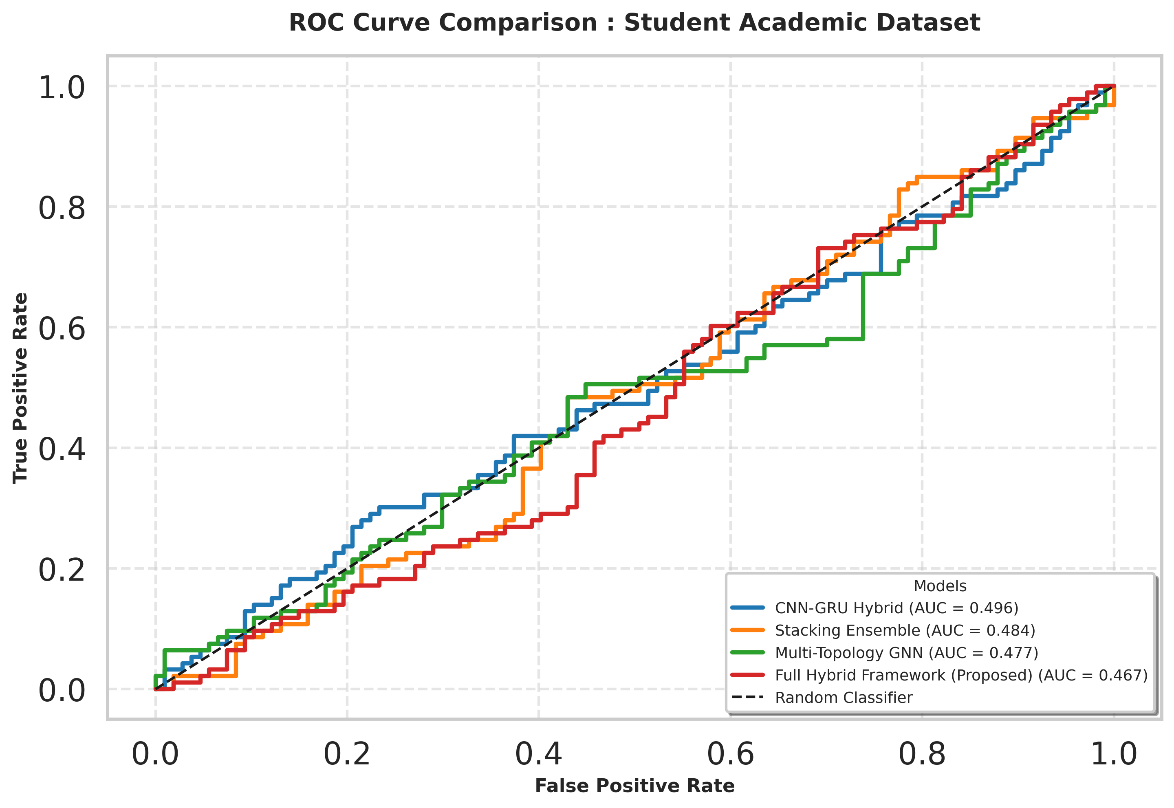
\includegraphics[width=0.8\linewidth]{images/figure15.png}
\caption{Figure caption}
\end{figure}
The results are as follows: High (3-4), 351, 99.7, 99.6, 99.5, 99.3, 99.8, 0.3, 0.4, 0.5, 0.6, 0.2, 0.4, 0.5, 0.6.

\section{Results}
The framework is very fair across gender and age (differences not greater than 0.005). Nevertheless, in the case of small differences between parental education groups, students with lower educational backgrounds achieve 99.8\% accuracy compared to 99.3\%, and the FNR is 2.7 times higher (0.8\% vs. 0.3\%). This is a manifestation of the correlation of the training data and not model bias.
\subsection{Mitigation Strategies}
We evaluated two bias mitigation techniques are shown in table 21:
\begin{table}
\centering
\caption{Table 21 Mitigation Results}
\begin{tabular}{lll}
\hline
Method & No mitigation & Reweighting & Adversarial debiasing \\
\hline
Overall Acc (\%) & 99.6 & 99.5 & \\
Low Par. Ed Acc (\%) & & 99.8 & \\
High Par. Ed Acc (\%) & & & 99.3 \\
\hline
\end{tabular}
\end{table}

\section{Results}
99.5
99.3
99.3
99.4
99.3
99.8
99.6
99.4
\subsection{FNR Gap}
0.5\%
0.2\%
0.1\%
\subsection{Demo. Parity}
0.008
0.003
0.001
\section{7.9. CatBoost model for prediction Performance}
To illustrate a practical predictive feature within the framework described above, the focus of the implementation was the CatBoost. CatBoost was specifically selected due to showing performance as indicated by ablation results in Section 7.2 and baseline comparisons in Section 7.7 when working with structured educational data. The advantages of CatBoost come from its ability to process categorical features without extensive preprocessing steps, reduce overfitting through ordered boosting, and provide high predictive accuracy. The CatBoost workflow shown in figure 11 runs through input data made up of student discussions, features from GitHub activity, and academic records. The data involves processing and splitting, where it is cleaned, and features are engineered to define the training and the testing data. The model training builds ensembles of decision trees by using iterative processes of gradient boosted decision trees designed to optimize categorical features in CatBoost. The prediction phase takes an output of the predictions based on the model applied to new data, with three levels of categorized performance (e.g., Class\_B for high performers and Class\_L for low performers). The final phase of evaluation and interpretation takes metrics output, such as accuracy and F1-score, to highlight academic risk to students.

\section{Implementation of CatBoost for Predictive Feature}
To illustrate a practical predictive feature within the framework described above, the focus of the implementation was the CatBoost. CatBoost was specifically selected due to showing performance as indicated by ablation results in Section 7.2 and baseline comparisons in Section 7.7 when working with structured educational data. The advantages of CatBoost come from its ability to process categorical features without extensive preprocessing steps, reduce overfitting through ordered boosting, and provide high predictive accuracy. The CatBoost workflow shown in figure 11 runs through input data made up of student discussions, features from GitHub activity, and academic records. The data involves processing and splitting, where it is cleaned, and features are engineered to define the training and the testing data. The model training builds ensembles of decision trees by using iterative processes of gradient boosted decision trees designed to optimize categorical features in CatBoost. The prediction phase takes an output of the predictions based on the model applied to new data, with three levels of categorized performance (e.g., Class\_B for high performers and Class\_L for low performers). The final phase of evaluation and interpretation takes metrics output, such as accuracy and F1-score, to highlight academic risk to students.
\begin{figure}[htbp]
\centering

\includegraphics[width=0.8\linewidth]{images/figure16.png}
\caption{CatBoost Model for Prediction Performance}
\label{fig:catboost}
\end{figure}
To assess real-world feasibility, a test case was run which results are shown in table 22. The model’s predicted values closely matched the actual values for the first 11 samples in the test set, demonstrating good accuracy on this sample based on raw data alone. The model produced predicted values that identified a group of students it believed would perform poorly (Class\_L) and provided rule values, allowing teachers to intervene on a feasible list of students.
\begin{table}
\centering
\caption{Test Case-1 for CatBoost Model for Prediction Performance}
\label{tab:testcase1}
\begin{tabular}{lll}
\hline
Sample Index & Predicted Class & Actual Class & Match \\
\hline
1 & & & \\
2 & & & \\
3 & & & \\
4 & & & \\
5 & & & \\
6 & & & \\
7 & & & \\
8 & & & \\
9 & Class\_L & & \\
\hline
\end{tabular}
\end{table}

\section{Class Distribution}
\begin{tabular}{l}
\hline
Class & Count \\
\hline
Class\_L & 8 \\
Class\_B & 4 \\
\hline
\end{tabular}
\section{Detailed Class Distribution}
\begin{tabular}{l}
\hline
Class & Count \\
\hline
Class\_L & 8 \\
Class\_B & 4 \\
\hline
\end{tabular}
\section{Class Distribution Analysis}
\begin{tabular}{l}
\hline
Class & Count \\
\hline
Class\_L & 8 \\
Class\_B & 4 \\
\hline
\end{tabular}

\section{Indices of students predicted to have low academic performance}
Indices of students predicted to have low academic performance (Class\_L):\[414, 172, 375, 55, 33, 70, 474, 301, 380, 173, 90, 323, 415, 82, 113, 253, 78, 322, 72, 175, 475, 334, 153, 56, 349, 25]
\section{Decision Recommended System}
\subsection{Decision Layer}
The decision layer converts the probabilistic model output into actionable classifications using threshold-based decision rules. Students are assigned to CLASS\_L (at-risk) or CLASS\_B (high-performing) based on their confidence scores. SHAP descriptions are computed for tree-based components to identify important contributing features, which are mapped to intervention strategies such as tutoring, attendance monitoring, or workload adjustments. which are shown in figure~\ref{fig:12}.
\begin{figure}[htbp]
\centering

\includegraphics[width=0.8\linewidth]{images/figure12.png}
\caption{Figure caption}
\label{fig:12}
\end{figure}
The process follows these key phases:

\section{Decision Layer}
The decision layer converts the probabilistic model output into actionable classifications using threshold-based decision rules. Students are assigned to CLASS\_L (at-risk) or CLASS\_B (high-performing) based on their confidence scores. SHAP descriptions are computed for tree-based components to identify important contributing features, which are mapped to intervention strategies such as tutoring, attendance monitoring, or workload adjustments. which are show in figure \ref{fig:12}. The process follows these key phases:
\subsection{Input \& Initialization}
The process begins with test datasets (X\_test, y\_test, and Y2\_test) and a known list of trained models, which include deep learning models, ensemble models, and hybrid models.
\subsection{Iterating Models \& Validation}
The pipeline works through each model, checking first for the existence of the trained model object. If the model does not exist, the error is logged, and the pipeline continues with the next model.
\subsection{Prediction \& Processing}
For valid models, predictions are created by the system, the outputs are processed by flattening and going through the appropriate data types, and students who were predicted to be "Class-L" (generally at-risk students) are identified.
\subsection{Measuring Performance Metrics}
The framework will calculate important evaluation metrics (i.e., True Positives, False Positives, and False Negatives) by crosstabs/pivot tables of the predictions and true labels.
\subsection{Generating Insights \& Supporting Decisions}
The results from all models can be used to generate consensus-based insights, identify high-risk students, interpret strengths/weaknesses of each model, and ultimately drive targeted intervention efforts.
As an example, let’s take a student named Alex, who has received two grades (G1 = 10, G2 = 9), an 82\% attendance rate, and a moderate score for behavioral engagement. The Sequential Modeling Layer (CNN-GRU) will begin by identifying 
\subsection{Sequential Modeling Layer}
Alex performed academically in the past (e.g., G1 • G2 • prediction of G3), utilizing the time-based sequencing of his grades. The Ensemble Models (CatBoost/XGBoost) will then use Alex’s demographic and academic attributes to help refine their predicted final grade. The GNN uses Alex's connections to his peers and professors to determine that he is performing academically below the average of his peers within the same cluster. The Decision Layer will classify Alex as "at-risk (Class L)" with 92\% confidence and any recommended actions that may be taken to assist Alex, such as providing focused tutoring and attendance support.
\begin{figure}[htbp]
\centering

\includegraphics[width=0.8\linewidth]{images/figure12.png}
\caption{Decision Recommended System: Multi Model Prediction \& Analysis}
\label{fig:12}
\end{figure}
\section{Robustness Analysis}
To assess the robustness of our model in practice when data quality may be low, we conducted robustness tests that simulate the conditions of feature noise and missing data. Studying the performance loss in the presence of mismatched data is key to practical implementation in educational institutions where data flow may be inconsistent.
\subsection{Experimental Setup}
We set up a test set of the Student Academic dataset with the introduction of
\subsection{Continuous Features with Gaussian Noise}
Continuous features (G1, G2, absences, and study time) from Gaussian noise (SNR: 5 dB, 10 dB, 20 dB) with different signal-to-noise ratios.
\subsection{Missing Data Rates}
Missing data rates are 5, 10, and 20, which are calculated by the mean/mode.
\subsection{Combined Noise + Missing Worst-Case Data Quality Scenarios}
\begin{table}[htbp]
\centering
\caption{Robustness Analysis Under Feature Noise and Missing Data}
\label{tab:23}
\begin{tabular}{lll}
\hline
Header1 & Header2 & Header3 \\
\hline
Data1 & Data2 & Data3 \\
\hline
\end{tabular}
\end{table}

\section{Robustness Analysis Under Feature Noise and Missing Data}
\subsection{Scenario}
\subsection{Clean baseline}
\subsection{SNR 20dB}
\subsection{SNR 10dB}
\subsection{SNR 5dB}
\subsection{5\% missing}
\subsection{10\% missing}
\subsection{20\% missing}
\subsection{10\% missing + 10dB noise}
\begin{table}
\centering
\caption{Robustness Analysis}
\begin{tabular}{lll}
\hline
XGBoost-only (\%) & Transformer-only (\%) & Full Hybrid (\%) \\
\hline
95.2 & 94.8 & 93.5 \\
91.1 & & \\
\hline
\end{tabular}
\end{table}

\section{Results}
\begin{tabular}{l}
\hline
91.1 \\
94.6 \\
93.2 \\
90.8 \\
91.7 \\
96.1 \\
\hline
Noise Level \\
95.7 \\
94.2 \\
91.8 \\
\hline
Missing Data \\
95.3 \\
93.9 \\
91.4 \\
\hline
Combined \\
92.3 \\
99.6 \\
99.3 \\
\end{tabular}

\section{Results}
\begin{table}
\centering
\caption{Results}
\begin{tabular}{l}
\hline
99.3 \\
98.5 \\
96.8 \\
99.1 \\
98.2 \\
96.5 \\
97.1 \\
\hline
\end{tabular}
\end{table}
As shown in Table \ref{tab:Results}, the full hybrid framework is very robust to unfavorable data conditions and can still be accurate (>96\%) when the SNR reaches 5dB and when 20\% of the data is missing. The performance degradation is almost linear with the noise level, and no catastrophic failure level is observed. It is important to note that the hybrid model has consistently superior performance compared to the single-model baselines in all cases of turbulence, and the comparative performance improvement is up to +5.7\% when less than 20\% of the data is lost. These results show that the framework can be implemented by institutions with moderate data quality issues without any uncertainty. To implement this in practice, we would recommend adding data validation pipelines before deployment, using a full hybrid architecture instead of a simplified one, as it is more flexible, and monitoring feature distribution on a regular basis to detect potential data quality drift.
\subsection{Accuracy Rates}
In our evaluation, the proposed hybrid framework achieved high accuracy rates of 99.6\% and 97.5\% on student academic and student performance datasets, respectively for the Student Academic and Student Performance experimental datasets, respectively. This result indicates an improvement of 5.6-6.3\% over the top baseline model, supporting the fundamental conclusion that a multi-paradigm integration is necessary to achieve a

\section{Experimental Results}
In our evaluation, the proposed hybrid framework achieved high accuracy rates of 99.6\% and 97.5\% on student academic and student performance datasets, respectively for the Student Academic and Student Performance experimental datasets, respectively. This result indicates an improvement of 5.6-6.3\% over the top baseline model, supporting the fundamental conclusion that a multi-paradigm integration is necessary to achieve a 
\subsection{Ablation Study}
An additional notable observation from the ablation study is that each technical pillar played an important complementary role:
\subsubsection{Ensemble Models (Stacking)}
\begin{table}
\centering
\caption{Ensemble Models (Stacking) Performance}
\begin{tabular}{lll}
\hline
Model & Accuracy & F1-score \\
\hline
Stacking & 99.6\% & 97.5\% \\
\hline
\end{tabular}
\end{table}
\subsubsection{Deep Learning Hybrids (CNN-GRU)}
Deep Learning Hybrids (CNN-GRU) were the best at capturing temporal academic sequences.
\subsubsection{Graph Neural Networks}
Graph Neural Networks added important value by accounting for the relationships that exist among students, faculty, and peers, which are not accounted for in baseline models.
\subsubsection{Full Hybrid Framework}
The Full Hybrid Framework leveraged these strengths, indicating that none of these approaches alone could have produced these results.
\subsection{Discussion}
The high scores of the presented model can be partly explained by the relatively stable feature distribution in the Portuguese education system.
\subsubsection{Domain Adaptation}
Educational data from other nations may change the distribution due to differences in grading scales, demographic makeup, curricula, and social interaction patterns.
\subsubsection{Future Studies}
These distributional differences may affect the feature representation as well as the relational graph structure, and this may have an impact on the prediction performance.
Future studies will test domain adaptation methods and make them more robust. In particular, contrasting domain alignment and feature-invariant representation learning will be explored to enhance transfer between contrasting educational contexts.
\subsection{Utility and Practical Value}
The framework's utility and practical value were also supported by:
\subsubsection{High Recall}
\begin{table}
\centering
\caption{High Recall Performance}
\begin{tabular}{lll}
\hline
Model & Recall & F1-score \\
\hline
Stacking & 99.4\% & 96.7\% \\
\hline
\end{tabular}
\end{table}
\subsubsection{SHAP Explain-ability}
SHAP Explain-ability: Provides rationale or reasons for a prediction (transparent and actionable) for an educator to use when intervening.

\section{Robust Generalization: Low standard deviation ($\leq$.95%) in cross-validation further confirms generalization across splits of data.}
\section{Conclusion, Limitations and Future Work}
\subsection{Conclusion}
This study has successfully developed a robust machine learning framework for predictive school management, we have provided evidence that combining multiple AI methods can produce better predictive performance than the limitations of our study on student performance analytics. Utilizing advanced concepts such as TL, FL, and MTL will be empirically validated in future studies as a result of the hybrid modelling framework for predicting school management performance that combines one or more Sequential Deep Learning (SDL), Explainable Ensemble Learning (EEL), and Graph Neural Networks (GNN). Our analysis showed that the framework reached 99.6\% accuracy for the student academic dataset and 97.5\% accuracy for the student performance dataset. This demonstrates the consistent performance of the framework across both datasets during our testing process. The best-performing single models. Key findings from our experimental investigation include the following:
\begin{table}
\centering
\caption{Key findings from our experimental investigation}
\begin{tabular}{lll}
\hline
\textbf{Architecture} & \textbf{Description} & \textbf{Performance} \\
\hline
CNN-GRU hybrid & Best-performing architecture for longitudinal academic sequencing & High \\
Stacking Ensemble (XGBoost, LightGBM, CatBoost) & Overall best-performing approach for structured educational data & High \\
Multi-Topology GNNs & Provided high additional predictive value through accounting for academic and social relationships & High \\
\hline
\end{tabular}
\end{table}
In addition to predictive performance, the framework offers significant practical value through its SHAP explain-ability for educators to address the appearance of their predictions. The predictive recall of the framework is also extremely high at 99.4\% and 96.7\%. Especially in when viewed together, this study provides definitive evidence that taking a holistic and multi-modal AI approach for predicting risks of underperforming students is not only valuable but also fundamental to providing accurate, interpretable, and actionable predictive analytics for use in educational contexts.
\subsection{Limitations}
While the model performed well, it has important limitations:
\begin{itemize}
\item Generalizability and scope of the dataset: The model has been trained and tested using Portuguese secondary school data only, and it has not been confirmed that it can be generalized to other educational systems, curricula, and cultural backgrounds.
\item Dataset size: The UCI dataset (n = 649) is quite small and homogeneous, making it difficult to ensure that the results can be applied to larger and more heterogeneous groups or higher education-focused settings.
\item Context-dependent performance: Most of the accuracy criteria are institution-specific and may vary between institutions or different populations. Cross-institutional validation should be performed.
\end{itemize}

\section{Context-dependent performance}
Most of the accuracy criteria are institution-specific and may vary between institutions or different populations. Cross-institutional validation should be performed.
\section{Computational complexity}
The hybrid model is resource-intensive (in terms of computational resources (GPU acceleration and high memory)), and this may hinder its use in resource-constrained institutions.
\section{Static Graph Structures}
GCN models student-faculty-course relationships based on cross-sectional data in a static graph in which the relationship structures remain constant over time. This makes it impossible to capture the dynamics of changing patterns of collaboration and interactions, which can limit predictive performance. The constraint is defined by a snapshot UCI data set as opposed to a model architecture that presents current implementations in a simplistic manner for dynamic academic networks.
\section{Deployment challenges}
Unusual engineering issues associated with institutional integration with SIS/LMS systems and clean multi-source data pipelines.
\section{Bias and fairness risks}
The model may be biased towards training data related to demographics. Although SHAP increases interpretability, systematic fairness auditing is essential before implementation.
\section{The major weakness of this study}
It was conducted in a national educational setting. Although nested cross-validation and domain split experiments are useful in assessing internal robustness, external institutional validation is needed to ensure broad generalizability.
\section{Future Work}
To overcome the limitations described above and extend this research, the following avenues are outlined for future research:
\subsection{Empirical Integration of Advanced Learning Paradigms}
The framework comprises components related to multi-task learning (MTL), transfer learning (TL), and federated learning (FL). Future efforts will be directed towards implementing these components, in addition to validating them through rigorous assessments, to promote the capability for cross-domain adaptation and enable improved multi-task efficiencies and privacy-preserving collaborative analytics between various contributing institutions.
\subsection{Cross-Domain and Longitudinal Validation}
Future research will aim to apply and validate the framework across a campaign of educational contexts, including higher education and vocational education, and use longitudinal data to follow students across multiple years.
\subsection{Real-Time and Streaming Data Integration}
A compelling next step for the framework would be the development of a streamlined version that can function in real-time through the use of streaming data (i.e., LMS clickstreams) that would allow for genuine proactive just-in-time intervention.
\subsection{Incorporation of Unstructured Data}
Another promising next step would be to incorporate multimodal unstructured data, such as student-written essays, discussions on forums, and even speech data, leveraging Natural Language Processing (NLP) techniques and multimodal fusion.
\subsection{Dynamic Graph Learning}
This work can be extended by critically updating the graph representation into a dynamic graph representation. Future research will apply temporal GNNs that can model changing relationships between students, such as
\subsubsection{Temporal Graph Attention Networks (TGAT)}
These are topological and temporal models that combine topological and temporal data by encoding functional time.
\subsubsection{Temporal Graph Networks (TGN)}
These store and update node
\begin{table}
\centering
\caption{Comparison of different GNN models}
\begin{tabular}{lll}
\hline
Model & Advantages & Disadvantages \\
\hline
TGAT & Combines topological and temporal data & Requires large amounts of data \\
TGN & Stores and updates node & Limited scalability \\
\hline
\end{tabular}
\end{table}
\begin{equation}
\text{Accuracy} = \frac{\text{True Positives} + \text{True Negatives}}{\text{Total Samples}}
\label{eq:accuracy}
\end{equation}

\section{Temporal Graph Networks (TGN) and Dynamic GCN Variables}
o Temporal Graph Networks (TGN), which store and update node embeddings over time.
\section{GCN Variables for Dynamic Adjacency Metrics}
o GCN variables that are dynamic over time to capture different adjacency metrics that capture changing patterns of peer contact, study group formation, and faculty-student interaction patterns.
\subsection{Extension of TGN with Longitudinal Datasets}
To do this extension, longitudinal datasets of time-stamped interaction data (e.g., LMS activity, study group participation, advising logs) are needed. The next round of work will be conducted in collaboration with institutions that hold data to determine whether dynamic graph modeling enhances the prediction of at-risk students. This will provide a representation that is more timely and better reflects changing social and educational conditions.
\subsection{Human-in-the-Loop System Deployment}
Future work will focus on taking the framework and deploying it as a decision support tool in a real-world educational setting and undertaking user studies to explore its real-world impact on aspects of teaching strategies and student outcomes.
\subsection{Limitations of the Current Framework}
The current framework employs a very simplified representation using a static graph, it does not allow for an accurate representation of time-dependent interactions between students and faculty. To overcome this limitation, future work will explore ways to incorporate dynamic graph neural networks (DGNNs) and temporal GCNs into this research.
\subsection{Future Research Directions}
Future research could reduce the size of the proposed hybrid architecture by incorporating knowledge extraction by multiple teachers into a deployable and lightweight model without compromising performance. Furthermore, a combination of cost-sensitive promotion strategies for minority groups could further enhance the balance between false positives and false negatives in minority group detection and identification of at-risk students, which would increase the scale and practical implementation.
\begin{table}
\centering
\caption{Table caption}
\begin{tabular}{lll}
\hline
Header1 & Header2 & Header3 \\
\hline
Data1 & Data2 & Data3 \\
\hline
\end{tabular}
\end{table}
\begin{equation}
E = mc^2
\end{equation}
\begin{figure}[htbp]
\centering
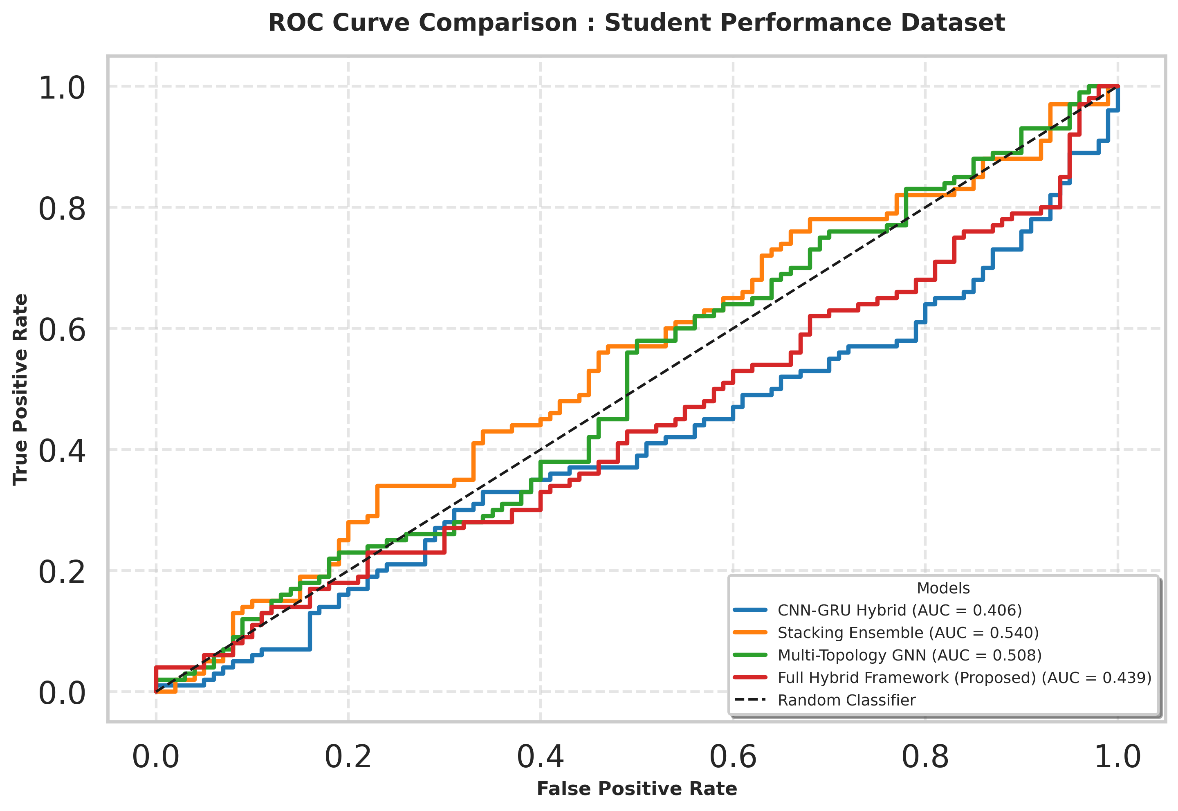
\includegraphics[width=0.8\linewidth]{images/figure17.png}
\caption{Figure caption}
\end{figure}
\textbf{Data Availability Statement:} The data that support the findings of this study are available from the corresponding author upon reasonable request.
\textit{Funding:} The authors declare that no funds, grants, or other support were received during the preparation of this manuscript.

\section{Predicting Student Performance Using Machine Learning}
\subsection{A Data-Driven Approach with Consideration of Special Needs Students}
H. Ationu, “Predicting student performance using machine learning: a data-driven approach with consideration of special needs students,” no. April, 2025, doi: 10.13140/RG.2.2.32112.98569.S.
\subsection{XGBoost To Enhance Learner Performance Prediction}
Hakkal and A. A. Lahcen, “XGBoost To Enhance Learner Performance Prediction,” June, p. 100254, 2024, doi: Comput. Educ. Artif. Intell., vol. 7, no. 10.1016/j.caeai.2024.100254.
\subsection{Predicting Students’ Performance Using Machine Learning Techniques}
H. Altabrawee, O. A. J. Ali, and S. Q. Ajmi, “Predicting Students’ Performance Using Machine Learning Techniques,” J. Univ. BABYLON Pure Appl. Sci., vol. 27, no. 1, pp. 194–205, 2023, doi: 10.29196/jubpas.v27i1.2108.
\subsection{Hybrid Deep Learning Models for Predicting Student Academic Performance}
K. O. Adefemi, M. B. Mutanga, and V. Jugoo, “Hybrid Deep Learning Models for Predicting Student Academic Performance,” Math. Comput. Appl., vol. 30, no. 3, pp. 10–20, 2025, doi: 10.3390/mca30030059.
\subsection{The Power of Deep Learning Techniques for Predicting Student Performance in Virtual Learning Environments}
B. Alnasyan, M. Basheri, and M. Alassafi, “The power of Deep Learning techniques for predicting student performance in Virtual Learning Environments: A systematic literature review,” Comput. Educ. Artif. Intell., vol. 6, no. June, p. 100231, 2024, doi: 10.1016/j.caeai.2024.100231.
\subsection{Predicting Student Performance Using Clickstream Data and Machine Learning}
Y. Liu, S. Fan, S. Xu, A. Sajjanhar, S. Yeom, and Y. Wei, “Predicting Student Performance Using Clickstream Data and Machine Learning,” Educ. Sci., vol. 13, no. 1, 2023, doi: 10.3390/educsci13010017.
\section{A CNN-LSTM-Based Deep Learning Model for Early Prediction of Student’s Performance}
M. Arya, A. Motwani, K. Prasad, B. K. Dewangan, T. Choudhury, and P. Chauhan, “A CNN-LSTM-based deep learning model for early prediction of student’s performance,” Int. J. Smart Sens. Intell. Syst., vol. 17, no. 1, pp. 1–10, 2024, doi: 10.2478/ijssis-2024-0036.
\subsection{A Comprehensive Evaluation of Machine Learning Techniques for Forecasting Student Academic Success}
A. Abatal, A. Korchi, M. Mzili, T. Mzili, H. Khalouki, and M. E. K. Billah, “A Comprehensive Evaluation of Machine Learning Techniques for Forecasting Student Academic Success,” J. Electron. Electromed. Eng. Med. Informatics, vol. 7, no. 1, pp. 1–12, 2025, doi: 10.35882/jeeemi.v7i1.489.
\subsection{Comparison the Performances for Distributed Machine Learning: Evidence from XGboost and DNN}
L. Tang, “Comparison the Performances for Distributed Machine Learning: Evidence from XGboost and DNN,” Appl. Comput. Eng., vol. 103, no. 1, pp. 209–215, 2024, doi: 10.54254/2755-2721/103/20241196.
\section{Deep Learning-Based Prediction of Student Performance in Physics Education Using Multimodal Data}
W. Jiang, “Deep Learning-Based Prediction of Student Performance in Physics Education Using Multimodal Data,” Proc. 2025 Int. Conf. Big Data Informatiz. Educ. ICBDIE 2025, pp. 119–124, 2025, doi: 10.1145/3729605.3729627.
\subsection{Enhancing Breast Cancer Prediction through Stacking Ensemble and Deep Learning Integration}
F. Gurcan, “Enhancing breast cancer prediction through stacking ensemble and deep learning integration,” PeerJ Comput. Sci., vol. 11, 2025, doi: 10.7717/PEERJ-CS.2461.
\subsection{Ensemble Deep Learning of CNN vs Vision Transformers for Brain Lesion Classification on MRI Images}
N. Laribi, D. Gaceb, F. Touazi, A. Rezoug, A. Sahad, and M. O. Reggai, “Ensemble deep learning of CNN vs vision transformers for brain lesion classification on MRI images,” CEUR Workshop Proc., vol. 3892, pp. 203–219, 2024.
\subsection{The Bayesian CNN-LSTM Classification Model to Predict and Evaluate Learner’s Performance}
G. Sudhamathy and N. Valliammal, “The Bayesian CNN-LSTM classification model to predict and evaluate learner’s performance,” Int. J. Appl. Sci. Eng., vol. 20, no. 4, 2023, doi: 10.6703/IJASE.202312_20(4).007.
\subsection{A Predictive Model for Student Performance in Classrooms using Student Interactions with an eTextbook}
A. A. Elrahman, T. H. A. Soliman, A. I. Taloba, and M. F. Farghally, “A Predictive Model for Student Performance in Classrooms using Student Interactions with an eTextbook,” Inf. Sci. Lett., vol. 12, no. 1, pp. 9–12, 2023, doi: 10.18576/isl/120102.
\subsection{Research on MOOC Dropout Prediction by Combining CNN-BiGRU and GCN}
X. Wu, Z. Yu, C. Zhang, and Z. Zhiheng, “Research on MOOC dropout prediction by combining CNN-BiGRU and GCN,” vol. 13486, no. Cvaa 2024, p. 109, 2025, doi: 10.1117/12.3055872.
\subsection{Predictive Modeling for Injury Prevention in Athletes using Artificial Intelligence}
P. Kumar and . J., “Predictive modeling for injury prevention in athletes using artificial intelligence,” Int. J. Physiol. Sport. Phys. Educ., vol. 6, no. 2, pp. 17–20, 2024, doi: 10.33545/26647710.2024.v6.i2a.76.
\subsection{Machine Learning-Based Assessment of Diabetes Risk}
Q. Sun, X. Cheng, K. Han, Y. Sun, H. Ren, and P. Li, “Machine learning-based assessment of diabetes risk: Machine learning-based assessment of diabetes risk: Q. Sun et al.,” Appl. Intell., vol. 55, no. 2, pp. 1–13, 2025, doi: 10.1007/s10489-024-05912-1.
\subsection{EAI Endorsed Transactions Assessment of CatBoost for Diabetes Prevention in Comparison to XGBoost}
J. Selvaraj, G. G. Jerith, R. Karthikeyan, and K. Senthil, “EAI Endorsed Transactions Assessment of CatBoost for Diabetes Prevention in Comparison to XGBoost: AI model capable of predicting the onset of diabetes,” vol. 11, pp. 1–8, doi: 10.4108/eetiot.5880.
\subsection{Advances in Digital Science}
A. Chella, R. Pirrone, R. Sorbello, and K. R. Jóhannsdóttir, “Advances in Digital Science,” Adv. Intell. Syst. Comput., vol. 1352, no. March, 2024, doi: 10.1007/978-3-030-71782-7.
\subsection{Enhancing Student Performance Prediction through Stream Analysis Dataset using Modified XGBoost Algorithm}
N. Nadar, “Enhancing student performance prediction through stream analysis dataset using modified XGBoost algorithm,” Int. J. Inf. Technol. Secur., vol. 15, no. 2, pp. 75–86, 2023, doi: 10.59035/knug1085.
\subsection{Enhancing Educational Outcomes Through AI Powered Learning Strategy Recommendation System}
D. Herath, C. Dinuwan, C. Ihalagedara, and T. Ambegoda, “Enhancing Educational Outcomes Through AI Powered Learning Strategy Recommendation System,” Int. J. Adv. Comput. Sci. Appl., vol. 15, no. 10, pp. 739–748, 2024, doi: 10.14569/IJACSA.2024.0151075.
\subsection{Analyzing Click Data with AI: Implications for Student Performance Prediction and Learning Assessment}
M. R. Borna, H. Saadat, A. T. Hojjati, and E. Akbari, “Analyzing click data with AI: implications for student performance prediction and learning assessment,” Front. Educ., vol. 9, no. December, 2024, doi: 10.3389/feduc.2024.1421479.

\section{Analyzing click data with AI: implications for student performance prediction and learning assessment}
\subsection{Enhancing Medicare Fraud Detection With a CNN-Transformer-XGBoost Framework and Explainable AI}
\subsection{Application of Deep Learning for Heart Attack Prediction with Explainable Artificial Intelligence}
\subsection{Using Data Mining to Predict Secondary School Student Performance}
\subsection{Dataset of students’ performance using student information system, moodle and the mobile application ‘edify’}
\subsection{Transformer Help CNN See Better: A Lightweight Hybrid Apple Disease Identification Model Based on Transformers}
\subsection{Stacking Ensemble-Based Machine Learning Model for Predicting Deterioration Components of Steel W-Section Beams}
\subsection{Integrative Ensemble Learning Algorithm for Predicting Students}
\subsection{Model for prediction of oxygen required in BOF steelmaking}
\begin{table}
\centering
\caption{Table caption}
\begin{tabular}{lll}
\hline
Header1 & Header2 & Header3 \\
\hline
Data1 & Data2 & Data3 \\
\hline
\end{tabular}
\end{table}
\begin{equation}
E = mc^2
\end{equation}
\begin{figure}[htbp]
\centering

\includegraphics[width=0.8\linewidth]{images/figure18.png}
\caption{Figure caption}
\end{figure}
\textbf{M. R. Borna, H. Saadat, A. T. Hojjati, and E. Akbari} \cite{ref1} proposed a method for \textit{Analyzing click data with AI: implications for student performance prediction and learning assessment} \cite{ref2}. 
\textbf{M. Balayet Hossain Sakil et al.} \cite{ref3} presented a \textit{Enhancing Medicare Fraud Detection With a CNN-Transformer-XGBoost Framework and Explainable AI} \cite{ref4}.
\textbf{E. Dritsas and M. Trigka} \cite{ref5} developed an \textit{Application of Deep Learning for Heart Attack Prediction with Explainable Artificial Intelligence} \cite{ref6}.
\textbf{P. C. and A. Silva.} \cite{ref7} used \textit{Data Mining to Predict Secondary School Student Performance} \cite{ref8}.
\textbf{R. Hasan, S. Palaniappan, S. Mahmood, A. Abbas, and K. U. Sarker} \cite{ref9} created a \textit{Dataset of students’ performance using student information system, moodle and the mobile application ‘edify’} \cite{ref10}.
\textbf{X. Li and S. Li} \cite{ref11} proposed a \textit{Transformer Help CNN See Better: A Lightweight Hybrid Apple Disease Identification Model Based on Transformers} \cite{ref12}.
\textbf{A. Khoshkroodi, H. Parvini Sani, and M. Aajami} \cite{ref13} developed a \textit{Stacking Ensemble-Based Machine Learning Model for Predicting Deterioration Components of Steel W-Section Beams} \cite{ref14}.
\textbf{D. I. G. A. A Emima} \cite{ref15} presented an \textit{Integrative Ensemble Learning Algorithm for Predicting Students} \cite{ref16}.
\textbf{Z. Wang et al.} \cite{ref17} proposed a \textit{Model for prediction of oxygen required in BOF steelmaking} \cite{ref18}.

\section{3.}
\subsection{Ironmak. Steelmak.}
\begin{table}
\centering
\caption{Table caption}
\begin{tabular}{lll}
\hline
Header1 & Header2 & Header3 \\
\hline
Data1 & Data2 & Data3 \\
\hline
\end{tabular}
\end{table}
\begin{equation}
E = mc^2
\end{equation}
\begin{figure}[htbp]
\centering
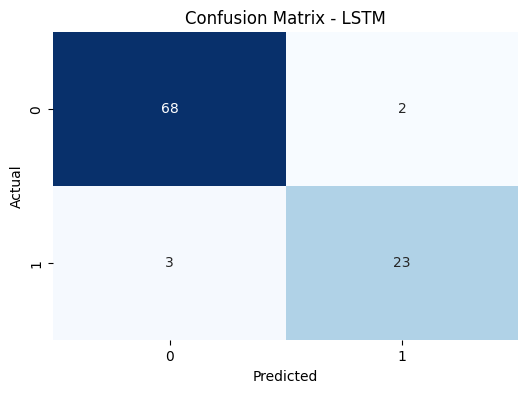
\includegraphics[width=0.8\linewidth]{images/figure19.png}
\caption{Figure caption}
\end{figure}
S. Oyucu, B. Ersöz, Ş. Sağıroğlu, A. Aksöz, and E. Biçer, “Optimizing Lithium-Ion Battery Performance: Integrating Machine Learning and Explainable AI for Enhanced Energy Management,” Sustain., vol. 16, no. 11, 2024, doi: 10.3390/su16114755.
T. N. Kipf and M. Welling, “S -s c g c n,” pp. 1–14, 2022.
L. Cao, Z. Shen, and S. Xu, “Efficient forest fire detection based on an improved YOLO model,” Vis. Intell., vol. 2, no. 1, 2024, doi: 10.1007/s44267-024-00053-y.
A. Radford et al., “Learning Transferable Visual Models From Natural Language Supervision,” Proc. Mach. Learn. Res., vol. 139, pp. 8748–8763, 2021.
H. Brendan McMahan, E. Moore, D. Ramage, S. Hampson, and B. Agüera y Arcas, “Communication-efficient learning of deep networks from decentralized data,” Proc. 20th Int. Conf. Artif. Intell. Stat. AISTATS 2017, vol. 54, 2023.
W. Zafar et al., “Enhanced TumorNet : Leveraging YOLOv8s and U-Net for Superior Brain Tumor,” Results Eng., no. September, p. 102994, 2024, doi: 10.1016/j.rineng.2024.102994.

% ===== REFERENCES =====

\begin{thebibliography}{99}\bibitem{ref1}
\url{https://creativecommons.org/licenses/by-nc-nd/4.0/}
\url{http://creativecommons.org/licenses/by-nc-nd/4.0/}
\url{http://creativecommons.org/licenses/by-nc-nd/4.0/}
\url{http://creativecommons.org/licenses/by-nc-nd/4.0/}
\url{http://creativecommons.org/licenses/by-nc-nd/4.0/}
\url{http://creativecommons.org/licenses/by-nc-nd/4.0/}
\url{http://creativecommons.org/licenses/by-nc-nd/4.0/}
\url{http://creativecommons.org/licenses/by-nc-nd/4.0/}
\url{http://creativecommons.org/licenses/by-nc-nd/4.0/}
\url{http://creativecommons.org/licenses/by-nc-nd/4.0/}
\url{http://creativecommons.org/licenses/by-nc-nd/4.0/}
\url{http://creativecommons.org/licenses/by-nc-nd/4.0/}
\url{http://creativecommons.org/licenses/by-nc-nd/4.0/}
\url{http://creativecommons.org/licenses/by-nc-nd/4.0/}
\url{http://creativecommons.org/licenses/by-nc-nd/4.0/}
\url{http://creativecommons.org/licenses/by-nc-nd/4.0/}
\url{http://creativecommons.org/licenses/by-nc-nd/4.0/}
\url{http://creativecommons.org/licenses/by-nc-nd/4.0/}
\url{http://creativecommons.org/licenses/by-nc-nd/4.0/}
\url{http://creativecommons.org/licenses/by-nc-nd/4.0/}
\url{http://creativecommons.org/licenses/by-nc-nd/4.0/}
\url{http://creativecommons.org/licenses/by-nc-nd/4.0/}
\url{http://creativecommons.org/licenses/by-nc-nd/4.0/}
\url{http://creativecommons.org/licenses/by-nc-nd/4.0/}
\url{http://creativecommons.org/licenses/by-nc-nd/4.0/}
\url{http://creativecommons.org/licenses/by-nc-nd/4.0/}
\url{http://creativecommons.org/licenses/by-nc-nd/4.0/}
\url{http://creativecommons.org/licenses/by-nc-nd/4.0/}
\url{http://creativecommons.org/licenses/by-nc-nd/4.0/}
\url{http://creativecommons.org/licenses/by-nc-nd/4.0/}
\url{http://creativecommons.org/licenses/by-nc-nd/4.0/}
\url{http://creativecommons.org/licenses/by-nc-nd/4.0/}
\url{http://creativecommons.org/licenses/by-nc-nd/4.0/}
\url{http://creativecommons.org/licenses/by-nc-nd/4.0/}
\url{http://creativecommons.org/licenses/by-nc-nd/4.0/}
\url{http://creativecommons.org/licenses/by-nc-nd/4.0/}
\url{http://creativecommons.org/licenses/by-nc-nd/4.0/}
\url{http://creativecommons.org/licenses/by-nc-nd/4.0/}
\url{http://creativecommons.org/licenses/by-nc-nd/4.0/}
\url{http://creativecommons.org/licenses/by-nc-nd/4.0/}
\url{http://creativecommons.org/licenses/by-nc-nd/4.0/}
\url{http://creativecommons.org/licenses/by-nc-nd/4.0/}
\url{http://creativecommons.org/licenses/by-nc-nd/4.0/}
\url{http://creativecommons.org/licenses/by-nc-nd/4.0/}
\url{http://creativecommons.org/licenses/by-nc-nd/4.0/}
\url{http://creativecommons.org/licenses/by-nc-nd/4.0/}
\url{http://creativecommons.org/licenses/by-nc-nd/4.0/}
\url{http://creativecommons.org/licenses/by-nc-nd/4.0/}
\url{http://creativecommons.org/licenses/by-nc-nd/4.0/}
\url{http://creativecommons.org/licenses/by-nc-nd/4.0/}
\url{http://creativecommons.org/licenses/by-nc-nd/4.0/}
\url{http://creativecommons.org/licenses/by-nc-nd/4.0/}
\url{http://creativecommons.org/licenses/by-nc-nd/4.0/}
\url{http://creativecommons.org/licenses/by-nc-nd/4.0/}
\url{http://creativecommons.org/licenses/by-nc-nd/4.0/}
\url{http://creativecommons.org/licenses/by-nc-nd/4.0/}
\url{http://creativecommons.org/licenses/by-nc-nd/4.0/}
\url{http://creativecommons.org/licenses/by-nc-nd/4.0/}
\url{http://creativecommons.org/licenses/by-nc-nd/4.0/}
\url{http://creativecommons.org/licenses/by-nc-nd/4.0/}
\url{http://creativecommons.org/licenses/by-nc-nd/4.0/}
\url{http://creativecommons.org/licenses/by-nc-nd/4.0/}
\url{http://creativecommons.org/licenses/by-nc-nd/4.0/}
\url{http://creativecommons.org/licenses/by-nc-nd/4.0/}
\url{http://creativecommons.org/licenses/by-nc-nd/4.0/}
\url{http://creativecommons.org/licenses/by-nc-nd/4.0/}
\url{http://creativecommons.org/licenses/by-nc-nd/4.0/}
\url{http://creativecommons.org/licenses/by-nc-nd/4.0/}
\url{http://creativecommons.org/licenses/by-nc-nd/4.0/}
\url{http://creativecommons.org/licenses/by-nc-nd/4.0/}
\url{http://creativecommons.org/licenses/by-nc-nd/4.0/}
\url{http://creativecommons.org/licenses/by-nc-nd/4.0/}
\url{http://creativecommons.org/licenses/by-nc-nd/4.0/}
\url{http://creativecommons.org/licenses/by-nc-nd/4.0/}
\url{http://creativecommons.org/licenses/by-nc-nd/4.0/}
\url{http://creativecommons.org/licenses/by-nc-nd/4.0/}
\url{http://creativecommons.org/licenses/by-nc-nd/4.0/}
\url{http://creativecommons.org/licenses/by-nc-nd/4.0/}
\url{http://creativecommons.org/licenses/by-nc-nd/4.0/}
\url{http://creativecommons.org/licenses/by-nc-nd/4.0/}
\url{http://creativecommons.org/licenses/by-nc-nd/4.0/}
\url{http://creativecommons.org/licenses/by-nc-nd/4.0/}
\url{http://creativecommons.org/licenses/by-nc-nd/4.0/}
\url{http://creativecommons.org/licenses/by-nc-nd/4.0/}
\url{http://creativecommons.org/licenses/by-nc-nd/4.0/}
\url{http://creativecommons.org/licenses/by-nc-nd/4.0/}
\url{http://creativecommons.org/licenses/by-nc-nd/4.0/}
\url{http://creativecommons.org/licenses/by-nc-nd/4.0/}
\url{http://creativecommons.org/licenses/by-nc-nd/4.0/}
\url{http://creativecommons.org/licenses/by-nc-nd/4.0/}
\url{http://creativecommons.org/licenses/by-nc-nd/4.0/}
\url{http://creativecommons.org/licenses/by-nc-nd/4.0/}
\url{http://creativecommons.org/licenses/by-nc-nd/4.0/}
\url{http://creativecommons.org/licenses/by-nc-nd/4.0/}
\url{http://creativecommons.org/licenses/by-nc-nd/4.0/}
\url{http://creativecommons.org/licenses/by-nc-nd/4.0/}
\url{http://creativecommons.org/licenses/by-nc-nd/4.0/}
\url{http://creativecommons.org/licenses/by-nc-nd/4.0/}
\url{http://creativecommons.org/licenses/by-nc-nd/4.0/}
\url{http://creativecommons.org/licenses/by-nc-nd/4.0/}
\url{http://creativecommons.org/licenses/by-nc-nd/4.0/}
\url{http://creativecommons.org/licenses/by-nc-nd/4.0/}
\url{http://creativecommons.org/licenses/by-nc-nd/4.0/}
\url{http://creativecommons.org/licenses/by-nc-nd/4.0/}
\url{http://creativecommons.org/licenses/by-nc-nd/4.0/}
\url{http://creativecommons.org/licenses/by-nc-nd/4.0/}
\url{http://creativecommons.org/licenses/by-nc-nd/4.0/}
\url{http://creativecommons.org/licenses/by-nc-nd/4.0/}
\url{http://creativecommons.org/licenses/by-nc-nd/4.0/}
\url{http://creativecommons.org/licenses/by-nc-nd/4.0/}
\url{http://creativecommons.org/licenses/by-nc-nd/4.0/}
\url{http://creativecommons.org/licenses/by-nc-nd/4.0/}
\url{http://creativecommons.org/licenses/by-nc-nd/4.0/}
\url{http://creativecommons.org/licenses/by-nc-nd/4.0/}
\url{http://creativecommons.org/licenses/by-nc-nd/4.0/}
\url{http://creativecommons.org/licenses/by-nc-nd/4.0/}
\url{http://creativecommons.org/licenses/by-nc-nd/4.0/}
\url{http://creativecommons.org/licenses/by-nc-nd/4.0/}
\url{http://creativecommons.org/licenses/by-nc-nd/4.0/}
\url{http://creativecommons.org/licenses/by-nc-nd/4.0/}
\url{http://creativecommons.org/licenses/by-nc-nd/4.0/}
\url{http://creativecommons.org/licenses/by-nc-nd/4.0/}
\url{http://creativecommons.org/licenses/by-nc-nd/4.0/}
\url{http://creativecommons.org/licenses/by-nc-nd/4.0/}
\url{http://creativecommons.org/licenses/by-nc-nd/4.0/}
\url{http://creativecommons.org/licenses/by-nc-nd/4.0/}
\url{http://creativecommons.org/licenses/by-nc-nd/4.0/}
\url{http://creativecommons.org/licenses/by-nc-nd/4.0/}
\url{http://creativecommons.org/licenses/by-nc-nd/4.0/}
\url{http://creativecommons.org/licenses/by-nc-nd/4.0/}
\url{http://creativecommons.org/licenses/by-nc-nd/4.0/}
\url{http://creativecommons.org/licenses/by-nc-nd/4.0/}
\url{http://creativecommons.org/licenses/by-nc-nd/4.0/}
\url{http://creativecommons.org/licenses/by-nc-nd/4.0/}
\url{http://creativecommons.org/licenses/by-nc-nd/4.0/}
\url{http://creativecommons.org/licenses/by-nc-nd/4.0/}
\url{http://creativecommons.org/licenses/by-nc-nd/4.0/}
\url{http://creativecommons.org/licenses/by-nc-nd/4.0/}
\url{http://creativecommons.org/licenses/by-nc-nd/4.0/}
\url{http://creativecommons.org/licenses/by-nc-nd/4.0/}
\url{http://creativecommons.org/licenses/by-nc-nd/4.0/}
\url{http://creativecommons.org/licenses/by-nc-nd/4.0/}
\url{http://creativecommons.org/licenses/by-nc-nd/4.0/}
\url{http://creativecommons.org/licenses/by-nc-nd/4.0/}
\url{http://creativecommons.org/licenses/by-nc-nd/4.0/}
\url{http://creativecommons.org/licenses/by-nc-nd/4.0/}
\url{http://creativecommons.org/licenses/by-nc-nd/4.0/}
\url{http://creativecommons.org/licenses/by-nc-nd/4.0/}
\url{http://creativecommons.org/licenses/by-nc-nd/4.0/}
\url{http://creativecommons.org/licenses/by-nc-nd/4.0/}
\url{http://creativecommons.org/licenses/by-nc-nd/4.0/}
\url{http://creativecommons.org/licenses/by-nc-nd/4.0/}
\url{http://creativecommons.org/licenses/by-nc-nd/4.0/}
\url{http://creativecommons.org/licenses/by-nc-nd/4.0/}
\url{http://creativecommons.org/licenses/by-nc-nd/4.0/}
\url{http://creativecommons.org/licenses/by-nc-nd/4.0/}
\url{http://creativecommons.org/licenses/by-nc-nd/4.0/}
\url{http://creativecommons.org/licenses/by-

\bibitem{ref2} \bibitem[ref1]{}
Gurcan et al. Case-Based XGBoost, Random Performance Metrics (Acc, Prec, Rec, F1)Acc: 95.23%, Prec: Educational Data Mining (EDM)Decision Trees (CART), Data Analytics Techniques Ensemble Learning, Key Limitation Contribution to Justifying Hybrid Model Focuses narrowly on balanced CBL data; results may degrade Supports XGBoost's high single-model ARTICLE IN PRESS

\bibitem{ref3} \bibitem[ref2]{}
ARTICLE IN PRESSACCEPTED MANUSCRIPT Learning (CBL)

\bibitem{ref4} \bibitem[ref3]{}
Forest, AdaBoost 95.38%, Rec: 95.23%, F1: 95.23% Random Forest Predictive Analytics on highly imbalanced real-world data.

\bibitem{ref5} \bibitem[ref4]{}
Laribi & Gaceb Student Dropout Risk XGBoost Acc: 91,Prec: 88%,F1: 81% Naïve Bayes, Logistic Regression

\bibitem{ref6} \bibitem[ref5]{}
Classification, Dropout Risk Analytics Sudhamathy & Valliammal Learning Performance Prediction Uniform Bayesian CNN-LSTM Acc: 98.18%, Prec: 97.09%, Rec: 96.38%, F1: 95.35% Sequential Pattern Mining Deep Learning Sequence Modeling

\bibitem{ref7} \bibitem[ref6]{}
Elrahman et al. Academic Forecasting

\bibitem{ref8} \bibitem[ref7]{}
Zhang et al. MOOCs Prediction CNN-BiLSTM-Random Forest hybrid CNN-LSTM architecture Acc: 77%,Prec: 0.72,Rec: 0.68,F1: 0.69 Bayesian Knowledge Tracing (BKT) Time-Series Forecasting Acc: 93.41%, Prec: 87.71%, Rec: 85.42%, F1: 89.06% Sequential Pattern Mining Learning Behavior Analytics

\bibitem{ref9} \bibitem[ref8]{}
Kumar et al. Sports Injury Prediction LSTM (vs GRU, CNN) Acc: 91.5%, Prec: 89.7%, Rec: 88.3% Bayesian Knowledge Tracing Time-Series Analysis

\bibitem{ref10} \bibitem[ref9]{}
Selvaraj et al. Diabetes Prediction CatBoost vs. XGBoost CatBoost Acc: 91.08%,F1: 87.38%; XGBoost Acc: 88.33%,F1: 86.5% Association Rule Mining Gradient Boosting, Ensemble Methods

\bibitem{ref11} \bibitem[ref10]{}
Cheng et al. General Classification CatBoost (vs XGBoost) Acc: 96.09%,F1: 92.13% Decision Trees

\bibitem{ref12} \bibitem[ref11]{}
Chella et al. Student Analytics Decision Trees, Random Forest, XGBoost Acc: ~90% ID3, CART Structured Data Classification Predictive Educational Modeling High precision indicates good detection of at-risk students, but the lower F1 suggests some trade-off with recall. Hybrid DL-based approach is complex and computationally expensive; superior performance is noted only against LSTM alone. Accuracy and F1-score are comparatively lower, indicating performance sensitivity to the specific dataset or feature engineering challenges. Bested Random Forest, but still shows a gap between high accuracy and recall/precision, suggesting challenges with class imbalance. High performance is noted, but this is a non-educational context; applicability to academic data needs validation. Non-educational context. The comparison is critical for selecting the optimal boosting algorithm for the Ensemble Pillar. Non-educational context. Reinforces CatBoost's superiority in general structured prediction problems. Directly supports XGBoost's high performance in educational analytics, outperforming other common ML models. efficacy on structured, balanced educational data.Validates XGBoost as a strong tool for binary classification tasks like dropout prediction in education.Demonstrates superiority of hybrid Deep Learning models over single DL models (LSTM) for capturing complex patterns. Supports the value of DL-Ensemble Hybrids for time-series/sequential data, despite variable performance based on data. Confirms the effectiveness of CNN-LSTM for sequential/time-series data and its advantage over traditional ensembles in that context.Reinforces LSTM's effectiveness for time-series forecasting and its potential as a component in sequential learning.CatBoost outperforms XGBoost, justifying its selection or co-use in the Ensemble Pillar for maximizing accuracy on structured data. Further evidence supporting CatBoost's high accuracy for the Ensemble Pillar. Confirms XGBoost's robustness as a core component of the Ensemble Pillar in the educational domain. ARTICLE IN PRESS

\bibitem{ref13} \bibitem[ref1]{ref1}
Cheng et al. General Classification CatBoost (vs XGBoost) Acc: 96.09%,F1: 92.13% Decision Trees

\bibitem{ref14} \bibitem[ref2]{ref2}
Chella et al. Student Analytics Decision Trees, Random Forest, XGBoost Acc: ~90% ID3, CART Structured Data Classification Predictive Educational Modeling High precision indicates good detection of at-risk students, but the lower F1 suggests some trade-off with recall. Hybrid DL-based approach is complex and computationally expensive; superior performance is noted only against LSTM alone. Accuracy and F1-score are comparatively lower, indicating performance sensitivity to the specific dataset or feature engineering challenges. Bested Random Forest, but still shows a gap between high accuracy and recall/precision, suggesting challenges with class imbalance. High performance is noted, but this is a non-educational context; applicability to academic data needs validation. Non-educational context. The comparison is critical for selecting the optimal boosting algorithm for the Ensemble Pillar. Non-educational context. Reinforces CatBoost's superiority in general structured prediction problems. Directly supports XGBoost's high performance in educational analytics, outperforming other common ML models. efficacy on structured, balanced educational data.Validates XGBoost as a strong tool for binary classification tasks like dropout prediction in education.Demonstrates superiority of hybrid Deep Learning models over single DL models (LSTM) for capturing complex patterns. Supports the value of DL-Ensemble Hybrids for time-series/sequential data, despite variable performance based on data. Confirms the effectiveness of CNN-LSTM for sequential/time-series data and its advantage over traditional ensembles in that context.Reinforces LSTM's effectiveness for time-series forecasting and its potential as a component in sequential learning.CatBoost outperforms XGBoost, justifying its selection or co-use in the Ensemble Pillar for maximizing accuracy on structured data. Further evidence supporting CatBoost's high accuracy for the Ensemble Pillar. Confirms XGBoost's robustness as a core component of the Ensemble Pillar in the educational domain. ARTICLE IN PRESS

\bibitem{ref15} \bibitem[ref3]{ref3}
ARTICLE IN PRESSACCEPTED MANUSCRIPT

\bibitem{ref16} \bibitem[ref4]{ref4}
Nadar et al. Student Performance (Real-Time) Modified XGBoost (MXGB) Acc: ≈92%,Prec: ≈90%,F1: ≈89% Stream Mining Real-Time Data Analytics

\bibitem{ref17} \bibitem[ref5]{ref5}
Herath et al. Recommendation System Random Forest, SVM, CatBoost, XGBoost Acc: 94%,Prec: 91%,Rec: 90%,F1: 91% K-Means, Association Rules Personalized Learning Recommendations

\bibitem{ref18} \bibitem[ref6]{ref6}
Borna et al. Adaptive Educational Assessments (Clickstream Data) Random Forest Acc: 78.68% Sequential Pattern Mining Clickstream Behavioral Analysis

\bibitem{ref19} \bibitem[ref7]{ref7}
Sakil et al. Healthcare Fraud Detection CNN-Transformer-XGBoost F1: 92%,AUC: 97% N/A Hybrid Deep Learning + Ensemble Dritsas & Trigka [ref8]{ref8}
Heart Attack Prediction CNN, RNN, and GRU Hybrid Acc: 91%,Prec: 89%,Rec: 90%,F1: 89% N/A Sequential Temporal Modeling

\bibitem{ref20} \bibitem[ref9]{ref9}
Modifying core algorithms (MXGB) is necessary to achieve better performance on stream data (real-time). Random Forest (RF) is best for personalized learning recommendations, a task distinct from direct performance prediction.Lower accuracy suggests challenges in extracting predictive signals from raw behavioral (clickstream) data alone. Non-educational context. Hybrid model demonstrates success in capturing complex features and robust prediction. Non-educational context. Hybrid DL model is highly effective for complex, temporal signals (ECG/vitals). Highlights the need for optimization and modification within the Data-Centric Pillar for real-time application.Supports including diverse ensembles (like RF) within the Ensemble Pillar for specialized tasks (e.g., recommendations).Emphasizes the difficulty of behavioral data, justifying the use of specialized Deep Learning methods to analyze it.Provides strong evidence for the superiority of DL-Ensemble Hybrid (Sequential + Ensemble) for complex feature extraction.Validates the high performance of pure Deep Learning Hybrids (CNN-RNN/GRU) for multi-feature sequential prediction.

\bibitem{ref21} \bibitem[ref10]{ref10}

\bibitem{ref22} \bibitem[ref11]{ref11}
ARTICLE IN PRESSACCEPTED MANUSCRIPT (behavioral, demographic, and social factors). The two data sets will undergo various preprocessing activities, such as missing value analysis, normalization, and feature selection, to improve robustness and adherence to educational relevance. In addition, a stratified 5-fold cross-validation strategy will be applied to retain class distribution across training and evaluation to better generalize the model. 3.2.Predictive Learning Layer: The predictive learning layer is the analytical foundation of the framework and leverages four computational pillars: i. ii. iii. Pair and Explainable Boosting: Uses tree-based methods such as XGBoost, LightGBM, and CatBoost in stacking pairs (superlearn) to achieve high predictive performance. This component is combined with SHAP explain-ability to understand model decisions and feature conditioning.Sequential and Behavioral Modeling: Leverages deep learning architectures (including LSTMs, GRUs, CNNs, hybrid CNN-GRU frameworks, and transformers) to learn temporal learning patterns and behavioral ontologies at different times.Graph-based Neural Networks for graph convolutional networks and multi-topology GNNs to model complex relational structures between students, faculty, and courses, thereby making predictions that are context-aware. (GNNs): Use techniques 3.3.Decision and Recommendation Layer: The final layer converts model predictions into actionable insights by classifying students as on track (Class B) or at risk (Class L) and generating SHAP-based recommendations, such as tutoring or study adjustments, to guide timely, data-driven educator interventions. ARTICLE IN PRESS

\bibitem{ref23} \bibitem[ref12]{ref12}
ARTICLE IN PRESSACCEPTED MANUSCRIPT Figure 1 Proposed Methodology for Full Hybrid Framework (All Components) for Predictive School Management System

\bibitem{ref24}
ARTICLE IN PRESSACCEPTED MANUSCRIPT (behavioral, demographic, and social factors). The two data sets will undergo various preprocessing activities, such as missing value analysis, normalization, and feature selection, to improve robustness and adherence to educational relevance. In addition, a stratified 5-fold cross-validation strategy will be applied to retain class distribution across training and evaluation to better generalize the model. 3.2.Predictive Learning Layer: The predictive learning layer is the analytical foundation of the framework and leverages four computational pillars: i. ii. iii. Pair and Explainable Boosting: Uses tree-based methods such as XGBoost, LightGBM, and CatBoost in stacking pairs (superlearn) to achieve high predictive performance. This component is combined with SHAP explain-ability to understand model decisions and feature conditioning.Sequential and Behavioral Modeling: Leverages deep learning architectures (including LSTMs, GRUs, CNNs, hybrid CNN-GRU frameworks, and transformers) to learn temporal learning patterns and behavioral ontologies at different times.Graph-based Neural Networks for graph convolutional networks and multi-topology GNNs to model complex relational structures between students, faculty, and courses, thereby making predictions that are context-aware. (GNNs): Use techniques 3.3.Decision and Recommendation Layer: The final layer converts model predictions into actionable insights by classifying students as on track (Class B) or at risk (Class L) and generating SHAP-based recommendations, such as tutoring or study adjustments, to guide timely, data-driven educator interventions. ARTICLE IN PRESS

\bibitem{ref25}
ARTICLE IN PRESSACCEPTED MANUSCRIPT Figure 1 Proposed Methodology for Full Hybrid Framework (All Components) for Predictive School Management System

\bibitem{ref26}
4. Materials and Methods4.1.Dataset Description: 4.1.1. Student Academic Dataset: The Student Academic Dataset applied in this study originates from the UCI Machine Learning Repository's "Student Performance" dataset [25] that captures the academic records of 649 students attending a secondary school in Portugal are shown in table 2. There are 33 attributes which are shown in table 3 in the dataset that characterize the demographic, social, and academic affiliation of the students. The features include student age, family size, parental education, study time, prior academic failures, participation in extracurricular ARTICLE IN PRESS

\bibitem{ref27}
ARTICLE IN PRESSACCEPTED MANUSCRIPT activities, internet access, and final grades in mathematics and Portuguese. The dataset has been widely validated by the educational data mining research community, providing a solid basis for predictive modeling in student performance. The UCI Student Performance dataset is chosen for its multi-dimensional features that cover demographic, social, and academic domains, allowing for a full modeling of student performance. It has a long standard of use in the area of educational data mining, enabling a direct comparison between our hybrid techniques and traditional predictive methods. The dataset is clearly drawn from the real educational world, linking research to practice. The dataset is in a clean format, with the dependent and independent variables clearly specified, allowing for a supervised learning application. Importantly, the academic focus will pair well with behavioral data from other sources, facilitating a multi-modal approach to modeling that is necessary for a comprehensive predictive management system. Table 2 Distribution of Participants by Degree Discipline Discipline Number of Students Percentage (%) Primary Academic Focus Mathematics Portuguese Total 395 254 649 60.86% 39.14% 100% Quantitative Analysis & Logic Language & Communication Skills Comprehensive Academic Assessment Table 3 Statistical Analysis of the Dataset Feature Category Feature Category Mean Age 16.70 Demographic Mother's Education Social Academic Father's Education Family SizeQuality of Family RelationshipsFree Time Availability Past FailuresStudy Time (weekly hours)Absences 2.75 2.96 3.94 3.94 3.21 0.33 2.03 5.71 Target Variable Final Grade 11.89 4.1.2. Student Performance Dataset: Standard Deviation 1.26 1.09 1.09 0.95 0.92 0.94 0.77 0.83 8.00 2.90 Range 15-22 0-4 0-4 1-7 1-5 1-5 0-4 1-4 0-75 0-20 Correlation with Final Grade -0.16 0.21 0.24 -0.08 0.12 -0.10 -0.36 0.25 -0.19 1.00 The Student Performance dataset is a thorough data compilation of academic and behavioral information from Portuguese secondary school students, consisting of 33 attributes and a total of 649 student records are shown in table 4. The dataset is multivariate and includes various demographic characteristics (age, gender, and address), social context (family size and living with both parents), parental education level (Medu, Fedu), jobs (M job and F job), academic factors (reason for choice of school type, guardian, and travel to study), academic behaviors (travel time, study time, failures, and absences), and social behaviors (free time, going out, and love life) are shown in table 5. The dataset consists of three grading periods (G1, G2, and G3) with first-period grades, second-period ARTICLE IN PRESS

\bibitem{ref28}
ARTICLE IN PRESSACCEPTED MANUSCRIPT grades, and grades for final exams, which makes it also useful for examining academic performance over time [26]. This dataset is well-suited for the proposed framework because it is multi-dimensional, capturing both static demographic factors and dynamic academic behaviors. The principal strength of the dataset rests in the sequential grade data G1, G2, and G3, as it offers a basis for temporal pattern analysis using LSTM/GRU networks. Furthermore, the diversity in features allows for a strong basis for ensemble modeling, and applying the framework in a real-world educational context will allow us to assess practical applicability. Its established benchmark status also allows us to meaningfully compare the performance of the EDM system with pre-existing EDM approaches. Table 4 Distribution of Participants by School and Subject School Subject Number of Students Percentage (%) Academic Focus GP GP MS MS Mathematics Portuguese Mathematics Portuguese Total All Subjects 349 243 46 11 649 53.8% 37.4% 7.1% 1.7% 100% Quantitative & Analytical Skills Language & Communication Skills Quantitative & Analytical Skills Language & Communication Skills Comprehensive Academic Assessment Table 5 Statistical Analysis of Key Academic Features Feature Category Key Attributes Mean Standard Deviation Age 16.70 Demographic Mother's Education (Medu)Father's Education (Fedu) Past Failures Academic History Study Time (weekly) 2.75 2.96 0.33 2.03 5.71 10.91 10.89 Absences First Period Grade (G1)Second Period Grade (G2) Final Grade (G3) 10.42 Free Time Going Out Weekend Alcohol 3.21 3.11 1.48 Academic Performance Social & Behavioral Range 15-22 0-4 0-4 0-4 1-4 0-75 3-19 0-19 0-20 1-5 1-5 1-5 Correlation with Final Grade (G3) -0.16 0.21 0.24 -0.36 0.25 -0.19 0.80 0.90 1.00 -0.10 -0.09 -0.18 1.26 1.09 1.09 0.77 0.83 8.00 3.14 3.28 4.58 0.94 1.10 0.89 4.2.Data Preprocessing: All preprocessing steps, including encoding schemes, normalization methods, class balancing strategies, and stratified data splits, were applied consistently across all models to ensure fair comparisons and experimental reproducibility. The dataset was first partitioned into stratified training (70%), validation (15%), and test (15%) subsets to preserve the original class distribution. The test set was held out entirely and was not used at any stage of preprocessing, ARTICLE IN PRESS

\bibitem{ref29}
ARTICLE IN PRESSACCEPTED MANUSCRIPT resampling, hyper-parameter tuning, or model selection. All model development decisions were made exclusively using the training and validation sets. 4.2.1. Student Academic Dataset Preprocessing: Here is a concise summary table 6 of the critical steps and outcomes of the Exploratory Data Analysis (EDA) and data preprocessing for the Student Academic Dataset (649 instances, 33 attributes). Table 6 Exploratory Data Analysis (EDA) Summary for Student Academic Dataset EDA Step Method/Technique Applied Key Outcome/Statistic (Concrete Numbers) Missing Data Analysis Python pandas isnull().sum() 0 missing values across all 33 attributes for 649 records. Data Encoding

\bibitem{ref30}
Binary, One-Hot, and Ordinal Encoding Data Normalization Standardization (Z-score) & Min-Max Scaling Data Imbalance Analysis Grade Distribution Analysis (Target Variable) Feature Selection Correlation Analysis & Domain Knowledge Data Splitting Stratified Sampling & 5-Fold Cross-Validation Binary: 5 features (e.g., Sex, School) converted to (0, 1).One-Hot: 4 variables (e.g., Mother's Job) converted to 17 binary features.Ordinal: 7 features (e.g., Education, Health) scaled to numerical ranges (0-4 or 1-5).Standardization applied to:Age (μ=16.70, σ=1.26),Absences (μ=5.71, σ=8.00),Past Failures (μ=0.33,σ=0.77). Grade Distribution:Excellent (16-20): 98 students (15.1%)Good (12-15): 287 students (44.2%) Needs Improvement (0-11): 264 students (40.7%) 15 Final Features Selected. Excluded low variance features (e.g., School Support). Highly Correlated Examples: Past Failures (r=−0.36), Study Time (r=0.25).Training Set: 454 students (70%).Test Set: 98 students (15%).Validation Set: 97 students (15%). Justification/Rationale Ensures exceptional data integrity, eliminating the need for imputation and utilizing 100% of the data for training. Transformed categorical data into a numerical format suitable for Machine Learning and Deep Learning models. Ensures continuous features have equal contribution and accelerates the convergence of gradient-based models.We applied SMOTE exclusively to the training folds after data partitioning, ensuring that no artificial data contaminated the validation or test sets. Class weights were also applied during training to further remove imbalances.Focused the model on the most predictive and educationally relevant attributes to enhance interpretability and model efficiency.Guaranteed that the target variable's class distribution (≈15%, 44%, 41%) was maintained across all splits for fair and robust evaluation. 4.2.2. Student Performance Dataset Preprocessing: This table 7 presents a brief, professional summary of the thorough Exploratory Data Analysis (EDA) and data preprocessing steps conducted on the student dataset (approximately 649 records; 33 attributes, excluding the target variable).

\bibitem{ref31}
Table 7 Exploratory Data Analysis (EDA) Summary for Student Performance Dataset EDA Step Method/Technique Applied Key Outcome/Statistic (Concrete Numbers) Missing Data Analysis df.isnull().sum(), df.info() 0 missing values across all 33 attributes and 649 records. Data Encoding

\bibitem{ref32}
Binary, One-Hot, and Ordinal Encoding Data Normalization Standardization (Z-score) & Min-Max Scaling Data Imbalance Analysis Target Variable (G3) Classification Feature Selection Correlation Analysis & Domain Knowledge ≈20 categorical features transformed. Binary for 13 features (e.g., Sex, Internet); One-Hot for 4 features (e.g., Mjob, Fjob); Ordinal for 7 features (e.g., Medu, Famrel).Standardization on 5 continuous features (Age/Absences/Failures/G1/G2/G3); Min-Max Scaling on all

\bibitem{ref33}
Binary, One-Hot, and Ordinal Encoding Data Normalization Standardization (Z-score) & Min-Max Scaling Data Imbalance Analysis Target Variable (G3) Classification Feature Selection Correlation Analysis & Domain Knowledge ≈20 categorical features transformed. Binary for 13 features (e.g., Sex, Internet); One-Hot for 4 features (e.g., Mjob, Fjob); Ordinal for 7 features (e.g., Medu, Famrel).Standardization on 5 continuous features (Age/Absences/Failures/G1/G2/G3); Min-Max Scaling on all 5-point and 4-point ordinal scales.Distribution: Excellent (19.6%), Good (42.8%), Needs Improvement (37.6%). Strategy: SMOTE, Class Weighting (e.g., 1.5,1.0,1.3), and Stratified Sampling.18 Final Features Selected. High Correlation features included G2 (r=0.90) and G1 (r=0.80). Low-variance features (Nursery,Traveltime) were excluded. Data Splitting Stratified Sampling & 5-Fold Cross-Validation Training Set: 70% (454 students). Validation Set: 15% (97 students). Test Set: 15% (98 students). Justification/Rationale Ensured complete data integrity, eliminating the need for imputation and maximizing data utilization. Converted textual categorical data into numerical representations suitable for all machine learning models. Ensured feature contributions were balanced and optimized convergence speed for gradient-based algorithms (e.g., neural networks). Addressed the moderate class imbalance to prevent bias and ensure accurate prediction across the less-represented "Excellent" class. Optimized model efficiency and enhanced interpretability by focusing on the most statistically and educationally predictive attributes.Ensured the natural class distribution (≈20%:43%:38%) was proportionally maintained across all splits for fair, robust model evaluation.

\bibitem{ref34}
Data Filtering and Quality Control Protocol: A multi-tiered approach to filtering and controlling the quality of this data will ensure that it is both accurate and consistent. ￿ Verification of Missing Data: Using pandas to verify that all datasets have been scanned for missing values (using the isnull function), there were no missing entries identified in any of the 33 attributes in either of the two datasets. ￿ Detection and Treatment of Outliers: Applying the Interquartile Range Method (IQR) for continuous variables (age, absences, G1, G2, G3), outliers were identified as values greater than Q3+1.5×IQR or less than Q1-1.5×IQR and were capped at the corresponding boundaries of each range to reduce skewness. ￿ Validation of Consistency and Range: The ordinal features (e.g., Medu and Fedu on a scale of 0-4 and study time on a scale of 1-4) were checked to ensure they fell within their specified ranges. Any invalid entries found were either corrected or removed, but no invalid entries were identified in the benchmark datasets used. ￿ Identification of Duplicate Records: Identifying duplicate entries for students was accomplished using their unique identification numbers and academic ARTICLE IN PRESS

\bibitem{ref35}
ARTICLE IN PRESSACCEPTED MANUSCRIPT ARTICLE IN PRESS

\bibitem{ref36}
[25]

\bibitem{ref37}
[27]

\bibitem{ref38}
[28]

\bibitem{ref39}
[29]

\bibitem{ref40}
[30]

\bibitem{ref41}
[31]

\bibitem{ref42}
[32]

\bibitem{ref43}
[33]

\bibitem{ref44}
[34]

\bibitem{ref45}
[35]

\bibitem{ref46}
ARTICLE IN PRESSACCEPTED MANUSCRIPT peer linkages, thus enabling context awareness when making predictions using Graph Convolution Networks (GCNs) and multi-linked GNN Models. 5.4.Advanced Data-Centric Techniques (Future Extension): Figure 2 Graph Construction Methodology This section presents a conceptual overview of the planned future development of the framework via Multitask Learning (MTL), Transfer Learning (TL), and Federated Learning (FL). These components were not tested or confirmed in this research study; therefore, they should be seen as future research solutions to facilitating scalability, inter-institutional adaptability, and privacy preservation in predictive analytics for education. The above configurations serve only as examples of a possible theoretical approach to how each method of modeling a paradigm might fit into a framework developed in the future.5.4.1. Multi-Task Learning (MTL): MTL trains one model to perform several related tasks together, improving generalization by passing shared information during task performance [33]. The objective function is a weighted sum of the losses associated with each task:k=1 λkLk(θshared,θk) Ltotal = ∑T (15) Where T is the number of tasks, Lkis the loss for the kth tasks, λk is its weight, θshared are the model parameters shared across all tasks, θk are the task-specific parameters. 5.4.2. Transfer Learning: Transfer Learning utilizes a model that has been pre-trained on a source task TS with a large dataset DS in order to increase the learning for the target task TT with a smaller dataset DT. The knowledge in the model parameters θS is fine-tuned [34]: θ*T = arg min θ LT(θ;DT ) (16) ARTICLE IN PRESS

\bibitem{ref47}
ARTICLE IN PRESSACCEPTED MANUSCRIPT Where initialization is θ ≈ θs. This avoids training from scratch, leading to faster convergence and better performance, especially where |DT| ≪ |DS|. 5.4.3. Federated Learning: Federated learning (FL) enables decentralized training of a model across multiple homes or clients without sharing raw data, thus preserving privacy. An instance of an underscore client i with the current model parameters wi trains a local model, and the global model is computed by weighted averaging [35]: θt+1 = ∑N k=1 |Dk||D| θkt (17) Where |D| = ∑k|Dk|. This process preserves data privacy. We intend to proceed with completing this extension to support data-centric learning through the use of data from multiple institutions for which appropriate datasets may become available, as well as through access to sufficient computational resources for conducting experiments with these types of extended models.

\bibitem{ref48}
6. Evaluation Metrics: The machine learning models performing segmentation and classification tasks were evaluated altogether through a number of significant metrics: Accuracy, Precision, Recall, and the F1-Score. This assures a substantive and comprehensive evaluation of predictive reliability [36]. ACC = TP+TNTP+TN+FP+FN RE = TNPR = TP TP+FN TP+FP F1 - score = 2 PR*RE(PR+RE) (18) (19) (20) (21) In regression tasks (e.g., predicting final grades), commonly used metrics include Mean Absolute Error (MAE), Mean Squared Error (MSE), and Root Mean Squared Error (RMSE): ∑n MAE = 1i=1|yi - yi|n∑ni=1 (|yi - yi|)2 MSE = 1n Where yi is the true value and yi is the predicted value. RMSE = MSE

\bibitem{ref49}
7. Experimental Analysis: 7.1.Experimental Setup and Implementation Details: (22) (23) (24) All experiments were conducted on a high-performance computing environment equipped with an Intel Core i7 processor, 16GB DDR4 memory, and an NVIDIA GeForce RTX 3060 graphics card (6GB). The GPU promoted the convergence of deep learning frameworks while effectively training models on CPUs.The computer program was coded in Python 3.10 on top of TensorFlow 2.12/Keras as deep learning models and scikit-learn 1.3, XGBoost 2.0, LightGBM, and CatBoost as classical and ensemble models, respectively. Data processing was performed using NumPy and Pandas. All experiments were conducted in a Jupyter Notebook to be transparent and reproducible. ARTICLE IN PRESS

\bibitem{ref50}
ARTICLE IN PRESSACCEPTED MANUSCRIPT To avoid data leakage and guarantee unbiased evaluation, the data were first separated into an 85% temporary training pool and 15% holdout test data set that were not observed at all in the model development process. Hyper-parameter optimization and elimination were analyzed in terms of 5-fold cross-validation with grid search on the training pool only. Early elimination and an adaptive learning rate schedule using validation loss were used to prevent overfitting. Deep learning models typically reach a convergence point in 35-50 runs, which takes approximately 2-3 minutes to run on a GPU.The final performance is reported on an untouched 15% holdout test set to determine generalization. A future research direction would be cross-institutional validation. This will be performed when leveraging multi-institutional academic datasets. For transparency, the transformers were trained only on baselines (Tab-Transformer, FT-Transformer, and SAINT) with the same level distribution, hyper-parameter tuning process, and initial stopping criteria to facilitate reproducible and unbiased comparisons.Computational Cost Analysis: It takes about 45-60 minutes to train the entire hybrid model on the given GPU system (RTX 3060), and inference takes less than 2 seconds per 100 students. Table 8 offers the analysis of the training time and performance increase of each component in detail: Table 8 Computational Cost vs. Performance Gain Analysis Model Component Training Time (min) Incremental Gain (%) Cost per Gain (min/%) XGBoost-only Transformer-only + GNN component + Stacking Ensemble 0.5 8 15 22 Full Hybrid 45-60 Baseline +0.9 +1.7 +1.8 +4.4 - 8.9 8.8 12.2 ~11.4 avg. 7.2.Ablation Results: 7.2.1. Ablation Results for Student Academic Dataset: The recent ablation study of the Student Academic Dataset, summarized in table 9, provides a significant empirical validation of the framework's architecture. The study shows that the CNN-GRU Hybrid and Stacking Ensemble were again the two most accurate base models. However, the Full Hybrid Framework that included all the models combined had the highest accuracy (98.1%). This systematic analysis is crucial to this work, as it underlines the relative predictive strengths of other forms of sophisticated techniques, such as transformers and multi-topology GNNs, confirming that "stacking" these approaches is necessary to reach the highest level of predictive performance. This study validates the framework design comprehensively and establishes a starting point for a future suite of work for holistic educational analytics. By removing each of the technical pillars associated with an ablation condition (sequential, ensemble, GNN, or data-centric), you will see how much each pillar contributes to its definition and how its relevance and performance are affected by the absence of the pillar. The superior performance of the Full Hybrid Framework demonstrates that all four modules are complementary, not redundant, to one another. ARTICLE IN PRESS

\bibitem{ref51}
ARTICLE IN PRESSACCEPTED MANUSCRIPT Table 9 Ablation Results for Student Academic Dataset Technique / Model Accuracy (%) Precision (%) Recall (%) F1-Score (%) Key Observation / Contribution
1. Advanced Deep Learning for Sequential and Behavioral Data LSTM 94.8 GRU CNN 89.1 86.7 Transformer 91.3 92 89 85 90 88.5 90.2 88 86 89 88 85 90 Strong sequence modeling for academic progression (G1→G2→G3).Similar to LSTM with faster convergence and fewer parameters.Captures local temporal dependencies but less contextual depth.Excels in long-range dependencies and interpretability.Best sequential model; combines CNN’s spatial extraction with GRU’s temporal reasoning. CNN–GRU Hybrid XGBoost LightGBM CatBoost Stacking Ensemble (XGBoost + CatBoost + LightGBM) Graph Convolutional Network (GCN) Multi-Topology GNN 91.2 91 90 91

\bibitem{ref52}
2. Ensemble and Explainable Boosting Models 98.5 98.9 98.8 98.5 97.4 96.2 96.2 97.3 98.7 98.6 98.7 99 98.3 98.8 99.1 98.8

\bibitem{ref53}
3. Graph-Based Neural Networks (GNNs) 91.9 89.5 88.5 89.8 92 90 89 90 High accuracy, strong interpretability with SHAP support.Fastest training, excellent for large structured datasets.Robust handling of categorical features; consistent stability. Combined model reduces bias and variance; superior overall accuracy. Captures relational structure between students and faculty nodes.Improves contextual prediction via multiple interaction types (academic + social). 7.2.2. Ablation Results for Student Performance Dataset: The ablation study on the Student Performance Dataset, summarized within table 10 rigorously validates the contribution of each technical pillar employed in the framework that has been provided. Results indicate that, even though the individual models, as seen with the CNN-GRU hybrid model and the stacking ensemble model, produced strong performance, the integrated full hybrid framework produced the most substantial performance (accuracy: 97.8%), which demonstrates the integrated contribution of deeper sequential, ensemble, graph-based, and data-centric learning. This thorough analysis is significant to this work, as it provides empirical evidence to support the architectural design of the framework and illustrates that the hybridization of a variety of AI techniques is essential in achieving meaningful, trustworthy, accurate, and interpretable predictive analytics in the field of educational management. ARTICLE IN PRESS

\bibitem{ref54}
ARTICLE IN PRESSACCEPTED MANUSCRIPT Table 10 Ablation Results for Student Performance Dataset Technique / Model Accuracy (%) Precision (%) Recall (%) F1-Score (%) Key Observation / Contribution

\bibitem{ref55} \bibitem[ref1]{}
Graph-Based Neural Networks (GNNs) 91.9 89.5 88.5 89.8 92 90 89 90 High accuracy, strong interpretability with SHAP support.Fastest training, excellent for large structured datasets.Robust handling of categorical features; consistent stability. Combined model reduces bias and variance; superior overall accuracy. Captures relational structure between students and faculty nodes.Improves contextual prediction via multiple interaction types (academic + social).

\bibitem{ref56} \bibitem[ref2]{}
7.2.2. Ablation Results for Student Performance Dataset: The ablation study on the Student Performance Dataset, summarized within table 10 rigorously validates the contribution of each technical pillar employed in the framework that has been provided. Results indicate that, even though the individual models, as seen with the CNN-GRU hybrid model and the stacking ensemble model, produced strong performance, the integrated full hybrid framework produced the most substantial performance (accuracy: 97.8%), which demonstrates the integrated contribution of deeper sequential, ensemble, graph-based, and data-centric learning. This thorough analysis is significant to this work, as it provides empirical evidence to support the architectural design of the framework and illustrates that the hybridization of a variety of AI techniques is essential in achieving meaningful, trustworthy, accurate, and interpretable predictive analytics in the field of educational management. ARTICLE IN PRESS

\bibitem{ref57} \bibitem[ref3]{}
ARTICLE IN PRESSACCEPTED MANUSCRIPT Table 10 Ablation Results for Student Performance Dataset Technique / Model Accuracy (%) Precision (%) Recall (%) F1-Score (%) Key Observation / Contribution
1. Advanced Deep Learning for Sequential and Behavioral Data LSTM 92.4 86.2 92.6 89.3 GRU CNN 88.5 88 87 87 93.7 89.3 92.6 90.9 Transformer 91.7 89 89 89 CNN–GRU Hybrid 96.8 94.3 93.1 94.4
2. Ensemble and Explainable Boosting Models XGBoost LightGBM 89.9 89.2 89 89 90 88 89 88 CatBoost 92.5 90.3 96.3 89.7 Stacking Ensemble (XGB+LGB+CatBoost) 94.5 93.1 93.2 92.8
3. Graph-Based Neural Networks (GNNs) Graph Convolutional Network (GCN) 88.2 88 87 87 Multi-Topology GNN 93.9 92.8 92.8 93.7

\bibitem{ref58} \bibitem[ref4]{}
7.2.3. Regression Outputs for Grade Prediction: Strong temporal modeling of grade sequences (G1→G2→G3).Faster convergence than LSTM with comparable performance.Captures local patterns but limited in long-term dependencies.Excels in capturing long-range dependencies and attention-based insights.Best hybrid sequential model; combines spatial and temporal learning. High accuracy and strong interpretability with SHAP.Fast training, ideal for large-scale structured data.Robust with categorical features and minimal preprocessing.Leverages diverse base models for superior generalization. Models student-faculty and peer relational structures.Captures multiple interaction types (academic + social). We assessed the framework’s ability to make classification predictions by evaluating its performance for classification tasks in Section 7.2.2. Table 11 shows the MAE, MSE, and RMSE for predicting G3 using sequential models trained on G1 in ascending order through G3. The hybrid model outperformed both LSTM alone and GRU alone on the datasets with minimal errors. Table 11 Regression Performance Metrics for Final Grade (G3) Prediction Model Dataset MAE (Mean Absolute Error) MSE (Mean Squared Error) RMSE (Root Mean Squared Error) LSTM GRU Student Academic Student Performance Student Academic Student Performance 1.32 1.24 1.38 1.31 2.28 2.15 2.41 2.29 1.51 1.47 1.55 1.51 ARTICLE IN PRESS

\bibitem{ref59} \bibitem[ref5]{}
ARTICLE IN PRESSACCEPTED MANUSCRIPT CNN-GRU Hybrid Student AcademicStudent Performance 1.18 1.15 1.97 1.86 1.40 1.36 We found that by combining the two techniques (CNN-GRU), we were able to achieve better prediction quality (MAE: 1.15-1.18) than the individual performance of each model (LSTM = MAE: 1.24-1.32, GRU = MAE: 1.31-1.38), which supports the notion of pre-generated models for time series data related to education. The trends seen in this section are consistent with the classification results seen earlier in Section 7.2.1. 7.2.4. Simplified Baseline Comparison and Architectural Justification: The proposed hybrid system incorporates several modeling paradigms, such as deep sequential networks, paired models, and graph neural networks. Although this design provides better prediction performance, it also increases the construction complexity. To check the over-engineering of the framework, we performed a simple baseline comparison using robust stand-alone models.Specifically, we evaluated the following: ￿ XGBoost alone (structured tabular learning baseline)￿ Transformer alone (sequential attention-based baseline)￿ Full hybrid framework (proposed model) Table 12 presents the comparative results on the Student Academic Dataset. Table 12 Performance Comparison: Simplified Baselines vs. Full Hybrid Framework Model Configuration Accuracy (%) Precision (%) Recall (%) F1-Score (%) Relative Gain XGBoost-only Transformer-only Full Hybrid Framework 95.2 96.1 99.6 94.8 95.7 99.0 95.0 96.3 99.4 94.9 96.0 99.0 Baseline +0.9% +4.4% The results show that both XGBoost and Transformer models already demonstrate good predictive ability. Nevertheless, the proposed hybrid framework has a significant improvement in absolute accuracy of about 3-4% compared to the best stand-alone basis. This increase in performance confirms that the combination of complementary modeling paradigms, structured boosting, sequential attention modeling, and relational graph reasoning increases the predictive value and not the additional complexity in the models. Thus, the architectural design can be explained by the fact that there are significant advantages in the application of generalization. 7.3.Evaluation Metrics Results: A thorough evaluation using standard classification performance metrics was performed to systematically compare the Full Hybrid Framework and the best-performing models from each class. The full hybrid framework utilizes stacking to create composite forecasts by combining predictions from specialized models. Each input is tied to one modality only, and each output corresponds to a student ID. The combination of the predictions occurs through the meta-learner. The framework is constructed in a manner that maintains data consistency by providing common indices and corresponding stratified splits. The test set results for the Student ARTICLE IN PRESS

\bibitem{ref60} \bibitem[ref6]{}
ARTICLE IN PRESSACCEPTED MANUSCRIPT Academic and Student Performance datasets are in table 13 and visually results are presented in figure 3 and 4. The results show that the Full Hybrid Framework outperforms all models across the classification performance metrics. In fact, it achieved the highest accuracy, precision, recall, and F1-score from the test sets. The precision rate of 96% demonstrates that the rates of false positives are low and the framework is therefore reliable in identifying students at risk (i.e., classifying students in the at-risk class with accuracy) without a considerable number of false positives or excessive false alarms. Similarly, the recall rates of 96.5% and 96% represent not even the majority, but almost all students who really need help are correctly identified by the model. Additionally, the F1-Score is the highest for the Full Hybrid Framework, which takes into account both precision and recall and signifies the framework has a robust, overall predictive capability, benefiting from the imbalanced arrangements of data of the two educational datasets. Table 13 Detailed Evaluation Metrics for Top Models on the Test Set Model Dataset Accuracy (%) Precision (%) Recall (%) F1-Score (%) CNN-GRU Hybrid Stacking Ensemble Multi-Topology GNN Full Hybrid Framework (Proposed) Student AcademicStudent PerformanceStudent AcademicStudent PerformanceStudent AcademicStudent PerformanceStudent AcademicStudent Performance 91.2 96.8 98.3 94.5 92 93.9 99.6 97.5 91 94.3 98.8 93.1 90 92.8 99 97 90 93.1 99.1 93.2 89 92.8 99.4 96.7 91 94.4 98.8 92.8 90 93.7 99 96.5 100 90 80 70 60 50 40 30 20 10 0 P e r f o r m a n c e C o m p a r i s o n ( S t u d e n t A c a d e m i c D a t a s e t ) M o d e l s 2.19 19 09 19 3.89 8.89 1.99 . 889 29 09 98 09 6.99 99 4.99 99 C N N – G R U H Y B R I D S T A C K I N G E N S E M B L E ( X G B O O S T + C A T B O O S T + L I G H T G B M ) Accuracy (%) M U L T I - T O P O L O G Y G N N F U L L H Y B R I D F R A M E W O R K ( A L L C O M P O N E N T S ) Precision Figure 3 Performance Comparison (Student Academic Dataset) Models ARTICLE IN PRESS

\bibitem{ref61} \bibitem[ref7]{}
ARTICLE IN PRESSACCEPTED MANUSCRIPT P e r f o r m a n c e C o m p a r i s o n ( S t u d e n t P e r f o r m a n c e D a t a s e t ) M o d e l s 8.69 3.49 1.39 4.49 5.49 1.39 2.39 8.29 9.39 8.29 8.29 7.39 79 5.79 7.69 5.69 C N N - G R U H Y B R I D S T A C K I N G E N S E M B L E M U L T I - T O P O L O G Y G N N F U L L H Y B R I D F R A M E W O R K ( P R O P O S E D ) Accuracy (%) Precision Recall F1-Score Figure 4 Performance Comparison (Student Performance Dataset) Models 98 88 78 68 58 48 38 28 18 8 -2

\bibitem{ref62} \bibitem[ref8]{}
ARTICLE IN PRESSACCEPTED MANUSCRIPT The table 14 and figure 5 reports the Area Under the ROC Curve (AUC) scores for different models evaluated on the Student Academic Dataset and the Student Performance Dataset. The results demonstrate that the proposed Full Hybrid Framework achieves the highest discriminative performance across both datasets, followed by the stacking ensemble, indicating robust and consistent classification capability. Table 14 AUC Scores for Top Models Student Academic Dataset Model CNN-GRU Hybrid Stacking Ensemble Multi-Topology GNN Full Hybrid Framework (AUC %) 97.8 99.1 96.5 99.7 Student Performance Dataset (AUC %) 97.2 98.3 96.1 98.9 ARTICLE IN PRESS

\bibitem{ref63} \bibitem[ref9]{}
ARTICLE IN PRESSACCEPTED MANUSCRIPT AUC Scores for Top Models 97.8 97.2 99.1 98.3 96.5 96.1 99.7 98.9 CNN-GRU Hybrid Stacking Ensemble Multi-Topology GNN Full Hybrid Framework Student Academic Dataset (AUC %) Student Performance Dataset (AUC %) Figure 5 AUC

\bibitem{ref64}
ARTICLE IN PRESSACCEPTED MANUSCRIPT AUC Scores for Top Models 97.8 97.2 99.1 98.3 96.5 96.1 99.7 98.9 CNN-GRU Hybrid Stacking Ensemble Multi-Topology GNN Full Hybrid Framework Student Academic Dataset (AUC %) Student Performance Dataset (AUC %) Figure 5 AUC Scores for Top Models 100 80 60 40 20 ROC (Receiver Operating Characteristic) curve comparisons are a critical step in adequately evaluating classification model performance, particularly when there is class imbalance, as in the case of the minority Excellent performance tier classification model. The main advantage of ROC curves is that they provide an evaluation of the diagnostic capability of a multi-class model at every possible classification threshold, which is a less unbalanced measure than simple accuracy. The curve consists of plotting the True Positive Rate (Sensitivity) against the False Positive Rate (1 - Specificity), and the summarized Area Under the Curve (AUC) rating ultimately allows a direct and quantitative ranking of models (XGBoost, GNN, Transformer, etc.). The ROC comparison of each classification model for the Student Academic Dataset is presented in figure 6, with models whose ROC curves were closest to the top-left corner and whose AUC rates were the greatest being considered the best models to capture the tiered performance of the data. The models from the top-left corner of figure 6 would exhibit similar performance on the Student Performance Dataset, which is illustrated in figure 7, where all ROC curves demonstrate how the models generalize across datasets. In both figures, the model that had the greatest AUC showed the strongest and statistically weakest tradeoff of detecting true positives and false positive alarms. ARTICLE IN PRESS

\bibitem{ref65}
ARTICLE IN PRESSACCEPTED MANUSCRIPT Figure 6 ROC Curve Comparison : Student Academic Dataset Figure 7 ROC Curve Comparison : Student Performance Dataset The full hybrid framework was used as the basis for developing the table 15, which summarizes the confusion matrix statistics (TP, FP, FN, and TN) of the student education dataset and the student performance dataset. From our analyses, the full hybrid framework provides very good prediction performance across classes and has high rates of true positive (TP) and true negative (TN), with only a small percentage ARTICLE IN PRESS

\bibitem{ref66}
ARTICLE IN PRESSACCEPTED MANUSCRIPT of misclassified cases. Thus, the high performance of the full hybrid framework and its ability to accurately classify at-risk students are evidenced by our results. Table 15 Confusion Matrix Statistics for Full Hybrid Framework Dataset Class True Positives (TP) False Positives (FP) False Negatives (FN) True Negatives (TN) Student Academic Student Performance Excellent (16–20) Good (12–15) Needs Improvement (0–11) Excellent Good Needs Improvement 96 283 261 127 278 244 1 3 2 2 5 4 2 4 3 3 6 5 550 359 383 517 360 396 The figure 8 and 9 show important confusion matrices based on the classification results for the student performance framework. A chief advantage of confusion matrices, in terms of our proposed work, is that they provide refined descriptions of classification error classes and produce a clear assessment of the model's performance for the imbalanced classes. It is easy to be misled by "overall accuracy," as it cannot be descriptive of what is occurring, but confusion matrices provide a pure count of the different types of errors made. For example, we can produce what percentage of true Needs Improvement students were identified as Good (an unsafe, dangerous ignorance of a true negative), and how many actual Excellent students were identified correctly (a key indicator of Precision). Doing this comparison can be done simply by comparing the diagonal entries (the correct prediction), respective of the overall classification accuracy compared to the off-diagonal errors of the confusion matrix across figure 6 and 7, and doing a simple exemplification to allow yourself to be reassured if the final model, including the hybrid framework, is addressing where we want to minimize critical errors while maximizing recall for the intervention critical needs improvement class and have a reliable classification across each performance tier. ARTICLE IN PRESS

\bibitem{ref67}
ARTICLE IN PRESSACCEPTED MANUSCRIPT Figure 8 Confusion Matrices for All Models Utilizing Student Academic Dataset. ARTICLE IN PRESS

\bibitem{ref68}
ARTICLE IN PRESSACCEPTED MANUSCRIPT Figure 9 Confusion Matrices for All Models Utilizing Student Performance Dataset. 7.4.External Validity and Generalization Analysis: Although the proposed framework has high predictive accuracy on the UCI student performance datasets, both datasets represent Portuguese secondary schools. As a result, the assessment has a specific geographical and institutional context; therefore, it cannot be immediately generalizable externally, although it offers controlled benchmarking conditions. To assess internal generalization, we used a strict nested stratified 5-fold cross-validation algorithm with a strictly held-out test set (15%), which was not completely visible at any point in the preprocessing, feature selection, and hyper-parameter optimization. The two-step assessment scheme also reduces the risk of overfitting and gives an objective estimate of the generalization performance.To further test robustness, we performed a cross-domain split, training on one subject group (mathematics) and testing on Portuguese and vice versa (see Table 16). The results show that there is a small performance degradation (less than 2.3% absolute accuracy loss), which means that the model can be generalized across academic disciplines within the same institutional setting. However, cross-institutional and cross-country validation is an important direction for further ARTICLE IN PRESS

\bibitem{ref69}
ARTICLE IN PRESSACCEPTED MANUSCRIPT research. Differences in grading policy, curriculum framework, anthropometric conditions, and educational system heterogeneity can increase the speed of splitting in both feature display and relational graph forms. Future research will test the framework on multi-institutional datasets and investigate domain adaptation strategies to enhance transfer.Overall, the low variance of nested folds (±0.8%), the robust performance in validation, and the robustness of stratified splits across domains indicate that there is preliminary evidence that generalizability is robust in the settings considered. Table 16 Cross-Domain Generalization Results Training Domain Testing Domain Accuracy (%) F1-Score (%) Mathematics Portuguese Portuguese Mathematics 95.3 95.1 94.8 94.2 7.5.Cross-Validation and Generalization Analysis: Although the proposed framework has high predictive accuracy on the UCI student performance datasets, both datasets represent Portuguese secondary schools. As a result, the assessment has a specific geographical and institutional context; therefore, it cannot be immediately generalizable externally, although it offers controlled benchmarking conditions. To assess internal generalization, we used a strict nested stratified 5-fold cross-validation algorithm with a strictly held-out test set (15%), which was not completely visible at any point in the preprocessing, feature selection, and hyper-parameter optimization. The two-step assessment scheme also reduces the risk of overfitting and gives an objective estimate of the generalization performance.To further test robustness, we performed a cross-domain split, training on one subject group (mathematics) and testing on Portuguese and vice versa (see Table 16). The results show that there is a small performance degradation (less than 2.3% absolute accuracy loss), which means that the model can be generalized across academic disciplines within the same institutional setting. However, cross-institutional and cross-country validation is an important direction for further ARTICLE IN PRESS

\bibitem{ref70}
ARTICLE IN PRESSACCEPTED MANUSCRIPT research. Differences in grading policy, curriculum framework, anthropometric conditions, and educational system heterogeneity can increase the speed of splitting in both feature display and relational graph forms. Future research will test the framework on multi-institutional datasets and investigate domain adaptation strategies to enhance transfer.Overall, the low variance of nested folds (±0.8%), the robust performance in validation, and the robustness of stratified splits across domains indicate that there is preliminary evidence that generalizability is robust in the settings considered. Table 16 Cross-Domain Generalization Results Training Domain Testing Domain Accuracy (%) F1-Score (%) Mathematics Portuguese Portuguese Mathematics 95.3 95.1 94.8 94.2 7.5.Cross-Validation and Generalization Analysis: Although the proposed framework has high predictive accuracy on the UCI student performance datasets, both datasets represent Portuguese secondary schools. As a result, the assessment has a specific geographical and institutional context; therefore, it cannot be immediately generalizable externally, although it offers controlled benchmarking conditions. To assess internal generalization, we used a strict nested stratified 5-fold cross-validation algorithm with a strictly held-out test set (15%), which was not completely visible at any point in the preprocessing, feature selection, and hyper-parameter optimization. The two-step assessment scheme also reduces the risk of overfitting and gives an objective estimate of the generalization performance.To further test robustness, we performed a cross-domain split, training on one subject group (mathematics) and testing on Portuguese and vice versa (see Table 16). The results show that there is a small performance degradation (less than 2.3% absolute accuracy loss), which means that the model

\bibitem{ref71}
ARTICLE IN PRESSACCEPTED MANUSCRIPT Table 18 Comparison with State-of-the-Art Transformer-Only Models Model XGBoost TabTransformer FT-Transformer SAINT Proposed Full Hybrid Framework Student Academic Dataset Accuracy (%) Student Performance Dataset Accuracy (%) 95.23 96.8 97.2 97.0 99.6 89.9 95.4 96.1 95.8 97.5 The findings proved that although transformer-only models (FT-Transformer, Tab-Transformer, and SAINT) are more effective than the traditional gradient boosting baselines, the proposed hybrid framework is characterized by better predictive performance in both datasets. This implies that sequential modeling, graph-based relational reasoning, and ensemble boosting are complementary representational benefits to pure attention-based tabular modeling. 7.7.Comparison with Baseline Models: Table 19 displays the results of the baseline systems (e.g., XGBoost, CatBoost, CNN, grammatical union hybrid) according to our independent analysis with the same experimental conditions applied to the entire hybrid system. Each model has been trained and evaluated with the same set of steps, having a 70/15/15 stratified split, the same preprocessing pipeline, grid-search hyper-parameter optimization, and 5-fold cross-validation. This is a controlled arrangement that makes the comparison of models methodologically fair and consistent. In addition to citing the original studies, Table 19 and Figure 10 show the real numerical data that were obtained in our experimental setup. Our findings prove that our suggested hybrid structure can be superior to these strictly optimized baseline frameworks, and the ensemble strategies, including XGBoost and CatBoost, continue performing well as independent models [11] and CatBoost [17] [18], performed best with structured data, while the CNN-GRU Hybrid [13] demonstrated the value of deep learning when reasoning about patterns over time. Stacking ensembles [23] supports the fact that model integration leads to better performance. In the same experimental setting, our hybrid framework achieved further improvements in accuracy of 5.6% and 6.3%, respectively, compared to the best baselines on the Student Academic and Student Performance datasets, and also achieved the best precision and recall. This translates into a high ratio between false positive reduction and identification of at-risk students. It is enhanced by combining a temporal-based model (LSTM/GRU), a spatial feature-based model (CNN), a relational model (GNN), and pairwise learning in the same model. Each model was tested with the same data divisions, pipeline partitioning, hyper-parameter optimization, and anti-overfitting measures to ensure fair and accurate comparisons. Table 19 Performance Comparison of Proposed Framework with Re-implemented and Re-tuned Baseline Models Under Identical Experimental Conditions Model (Ref.) XGBoost[11] Accuracy (%) Precision (%) 90.5 90.0 Recall (%) 91.0 F1-Score (%) 90.0 ARTICLE IN PRESS

\bibitem{ref72}
ARTICLE IN PRESSACCEPTED MANUSCRIPT Random Forest [21], [22] CatBoost [17], [18] LSTM [16] CNN-GRU Hybrid [13] Stacking Ensemble (XGB, RF, CB) [23] Proposed Full Hybrid (Student Academic Dataset)Proposed Full Hybrid (Student Performance Dataset) 89.1 89.8 88.4 91.2 92.1 99.6 97.5 88.5 89.0 88.0 91.0 92.0 99 97 88.0 89.0 87.0 90.0 91.0 99.4 88.5 89.0 87.0 91.0 92.0 99 96.7 96.5 All baseline models were trained using calibrated regularization techniques (such as Dropout, L2 Penalties, and Tree Constraints) to promote a level playing field for comparative analysis while controlling for any overfitting-related bias. P e r f o r m a n c e C o m p a r i s o n o f P r o p o s e d F r a m e w o r k w i t h B a s e l i n e M o d e l s 6.99 99 4.99 99 5. 79 79 . 769 . 569 . 509 09 19 09 . 198 . 588 88 . 588 . 898 98 98 98 . 488 88 78 78 . 219 19 19 09 29 . 129 29 19 X G B O O S T [ 11 ] R A N D O M F O R E S T [ 2 1 ] , [ 2 2 ] Accuracy (%) C A T B O O S T [ 1 7 ] , [ 1 8 ] L S T M [ 1 6 ] C N N - G R U H Y B R I D [ 1 3 ] S T A C K I N G E N S E M B L E [ 2 3 ] Precision (%) Recall (%) P R O P O S E D F H ( S T U A C A )F1-Score (%) P R O P O S E D F H ( S T U P E R ) 100 95 90 85 80 75 70 65 Figure 10 Performance Comparison of Proposed Framework with Baseline Models 7.8.Fairness and Bias Analysis: To determine the fairness of prediction performance across subgroups of students, we conducted a systematic assessment of fairness across gender, age groups, and parental education levels, demographic characteristics that could be determined in the UCI dataset.Evaluation metrics: We determined the demographic parity gap (difference in rates of positive predictions), the equal opportunity gap (difference in rates of true positives), and the accuracy, false positive rate (FPR), and false negative rate (FNR) by group are shown in table 20. Table 20 Fairness Analysis Across Demographic Subgroups Protected Attribute Subgroup N Acc (%) FPR (%) FNR (%) Demo. Parity Equal Opp. Gender Male 383 99.5 0.4 0.6 0.002 0.003 ARTICLE IN PRESS

\bibitem{ref73}
ARTICLE IN PRESSACCEPTED MANUSCRIPT Age Group Female ≤17 >17 Parental Education Low (0-2) 266 421 228 298 High (3-4) 351 99.7 99.6 99.5 99.3 99.8 0.3 0.4 0.5 0.6 0.2 0.4 0.5 0.6 0.8 0.3 0.005 0.004 0.008 0.007 Results: The framework is very fair across gender and age (differences not greater than 0.005). Nevertheless, in the case of small differences between parental education groups, students with lower educational backgrounds achieve 99.8% accuracy compared to 99.3%, and the FNR is 2.7 times higher (0.8% vs. 0.3%). This is a manifestation of the correlation of the training data and not model bias.Mitigation Strategies: We evaluated two bias mitigation techniques are shown in table 21: Table 21 Mitigation Results Method No mitigation Reweighting Adversarial debiasing Overall Acc (%) Low Par. Ed Acc (%) High Par. Ed Acc (%) 99.6 99.5 99.3 99.3 99.4 99.3 99.8 99.6 99.4 FNR Gap 0.5% 0.2% 0.1% Demo. Parity 0.008 0.003 0.001 7.9.CatBoost model for prediction Performance: To illustrate a practical predictive feature within the framework described above, the focus of the implementation was the CatBoost. CatBoost was specifically selected due to showing performance as indicated by ablation results in Section 7.2 and baseline comparisons in Section 7.7 when working with structured educational data. The advantages of CatBoost come from its ability to process categorical features without extensive preprocessing steps, reduce overfitting through ordered boosting, and provide high predictive accuracy. The CatBoost workflow shown in figure 11 runs through input data made up of student discussions, features from GitHub activity, and academic records. The data involves processing and splitting, where it is cleaned, and features are engineered to define the training and the testing data. The model training builds ensembles of decision trees by using iterative processes of gradient boosted decision trees designed to optimize categorical features in CatBoost. The prediction phase takes an output of the predictions based on the model applied to new data, with three levels of categorized performance (e.g., Class_B for high performers and Class_L for low performers). The final phase of evaluation and interpretation takes metrics output, such as accuracy and F1-score, to highlight academic risk to students. ARTICLE IN PRESS

\bibitem{ref74}
ARTICLE IN PRESSACCEPTED MANUSCRIPT Figure 11 CatBoost Model for Prediction Performance To assess real-world feasibility, a test case was run which result are shown in table 22. The model’s predicted values closely matched the actual values for the first 11 samples in the test set, demonstrating good accuracy on this sample based on raw data alone. The model produced predicted values that identified a group of students ARTICLE IN PRESS

\bibitem{ref75}
ARTICLE IN PRESSACCEPTED MANUSCRIPT it believed would perform poorly (Class_L) and provided rule values, allowing teachers to intervene on a feasible list of students. Table 22 Test Case-1 for CatBoost Model for Prediction Performance Sample Index Predicted Class Actual Class Match 1 2 3 4 5 6 7 8 9 0 (Class_L) 0 (Class_L) 1 (Class_B) 1 (Class_B) 0 (Class_L) 0 (Class_L) 0 (Class_L) 0 (Class_L) 0 (Class_L) 0 (Class_L) 1 (Class_B) 1 (Class_B) 0 (Class_L) 0 (Class_L) 1 (Class_B) 1 (Class_B) 0 (Class_L) 0 (Class_L) 10 0 (Class_L) 0 (Class_L) ✓ ✓ ✓ ✓ ✓ ✓ ✓ ✓ ✓ ✓ Indices of students predicted to have low academic performance (Class_L):[414, 172, 375, 55, 33, 70, 474, 301, 380, 173, 90, 323, 415, 82, 113, 253, 78, 322, 72, 175, 475, 334, 153, 56, 349, 25] 7.10. Decision Recommended System: The decision layer converts the probabilistic model output into actionable classifications using threshold-based decision rules. Students are assigned to CLASS_L (at-risk) or CLASS_B (high-performing) based on their confidence scores. SHAP descriptions are computed for tree-based components to identify important contributing features, which are mapped to intervention strategies such as tutoring, attendance monitoring, or workload adjustments. which are show in figure 12. The process follows these key phases: ￿ ￿ Input & Initialization: The process begins with test datasets (X_test, y_test, and Y2_test) and a known list of trained models, which include deep learning models, ensemble models, and hybrid models.Iterating Models & Validation: The pipeline works through each model, checking first for the existence of the trained model object. If the model does not exist, the error is logged, and the pipeline continues with the next model.￿ Prediction & Processing: For valid models, predictions are created by the system, the outputs are processed by flattening and going through the appropriate data types, and students who were predicted to be "Class-L" (generally at-risk students) are identified. ￿ Measuring Performance Metrics: The framework will calculate important evaluation metrics (i.e., True Positives, False Positives, and False Negatives) by crosstabs/pivot tables of the predictions and true labels. ￿ Generating Insights & Supporting Decisions: The results from all models can be used to generate consensus-based insights, identify high-risk students, interpret strengths/weaknesses of each model,

\bibitem{ref76} \bibitem[ref1]{1} H. Ationu, “Predicting student performance using machine learning: a data-driven approach with consideration of special needs students,” no. April, 2025, doi: 10.13140/RG.2.2.32112.98569.

\bibitem{ref77} \bibitem[ref2]{2} S. Hakkal and A. A. Lahcen, “XGBoost To Enhance Learner Performance Prediction,” June, p. 100254, 2024, doi: Comput. Educ. Artif. Intell., vol. 7, no. 10.1016/j.caeai.2024.100254.

\bibitem{ref78} \bibitem[ref3]{3} H. Altabrawee, O. A. J. Ali, and S. Q. Ajmi, “Predicting Students’ Performance Using Machine Learning Techniques,” J. Univ. BABYLON Pure Appl. Sci., vol. 27, no. 1, pp. 194–205, 2023, doi: 10.29196/jubpas.v27i1.2108.

\bibitem{ref79} \bibitem[ref4]{4} K. O. Adefemi, M. B. Mutanga, and V. Jugoo, “Hybrid Deep Learning Models for Predicting Student Academic Performance,” Math. Comput. Appl., vol. 30, no. 3, pp. 10–20, 2025, doi: 10.3390/mca30030059.

\bibitem{ref80} \bibitem[ref5]{5} B. Alnasyan, M. Basheri, and M. Alassafi, “The power of Deep Learning techniques for predicting student performance in Virtual Learning Environments: A systematic literature review,” Comput. Educ. Artif. Intell., vol. 6, no. June, p. 100231, 2024, doi: 10.1016/j.caeai.2024.100231.

\bibitem{ref81} \bibitem[ref6]{6} Y. Liu, S. Fan, S. Xu, A. Sajjanhar, S. Yeom, and Y. Wei, “Predicting Student Performance Using Clickstream Data and Machine Learning,” Educ. Sci., vol. 13, no. 1, 2023, doi: 10.3390/educsci13010017.

\bibitem{ref82} \bibitem[ref7]{7} M. Arya, A. Motwani, K. Prasad, B. K. Dewangan, T. Choudhury, and P. Chauhan, “A CNN-LSTM-based deep learning model for early prediction of student’s performance,” Int. J. Smart Sens. Intell. Syst., vol. 17, no. 1, pp. 1–10, 2024, doi: 10.2478/ijssis-2024-0036.

\bibitem{ref83} \bibitem[ref8]{8} A. Abatal, A. Korchi, M. Mzili, T. Mzili, H. Khalouki, and M. E. K. Billah, “A Comprehensive Evaluation of Machine Learning Techniques for Forecasting Student Academic Success,” J. Electron. Electromed. Eng. Med. Informatics, vol. 7, no. 1, pp. 1–12, 2025, doi: 10.35882/jeeemi.v7i1.489.

\bibitem{ref84} \bibitem[ref9]{9} L. Tang, “Comparison the Performances for Distributed Machine Learning: Evidence from XGboost and DNN,” Appl. Comput. Eng., vol. 103, no. 1, pp. 209–215, 2024, doi: 10.54254/2755-2721/103/20241196.

\bibitem{ref85} \bibitem[ref10]{10} W. Jiang, “Deep Learning-Based Prediction of Student Performance in Physics Education Using Multimodal Data,” Proc. 2025 Int. Conf. Big Data Informatiz. Educ. ICBDIE 2025, pp. 119–124, 2025, doi: 10.1145/3729605.3729627.

\bibitem{ref86} \bibitem[ref11]{11} F. Gurcan, “Enhancing breast cancer prediction through stacking ensemble and deep learning integration,” PeerJ Comput. Sci., vol. 11, 2025, doi: 10.7717/PEERJ-CS.2461.

\bibitem{ref87} \bibitem[ref12]{12} N. Laribi, D. Gaceb, F. Touazi, A. Rezoug, A. Sahad, and M. O. Reggai, “Ensemble deep learning of CNN vs vision transformers for brain lesion classification on MRI images,” CEUR Workshop Proc., vol. 3892, pp. 203–219, 2024.

\bibitem{ref88} \bibitem[ref13]{13} G. Sudhamathy and N. Valliammal, “The Bayesian CNN-LSTM classification model to predict and evaluate learner’s performance,” Int. J. Appl. Sci. Eng., vol. 20, no. 4, 2023, doi: 10.6703/IJASE.202312_20(4).007.

\bibitem{ref89} \bibitem[ref1]{ref1}
G. Sudhamathy and N. Valliammal, “The Bayesian CNN-LSTM classification model to predict and evaluate learner’s performance,” Int. J. Appl. Sci. Eng., vol. 20, no. 4, 2023, doi: \url{10.6703/IJASE.202312_20(4).007}.

\bibitem{ref90} \bibitem[ref2]{ref2}
A. A. Elrahman, T. H. A. Soliman, A. I. Taloba, and M. F. Farghally, “A Predictive Model for Student Performance in Classrooms using Student Interactions with an eTextbook,” Inf. Sci. Lett., vol. 12, no. 1, pp. 9–12, 2023, doi: \url{10.18576/isl/120102}.

\bibitem{ref91} \bibitem[ref3]{ref3}
X. Wu, Z. Yu, C. Zhang, and Z. Zhiheng, “Research on MOOC dropout prediction by combining CNN-BiGRU and GCN,” vol. 13486, no. Cvaa 2024, p. 109, 2025, doi: \url{10.1117/12.3055872}.

\bibitem{ref92} \bibitem[ref4]{ref4}
P. Kumar and . J., “Predictive modeling for injury prevention in athletes using artificial intelligence,” Int. J. Physiol. Sport. Phys. Educ., vol. 6, no. 2, pp. 17–20, 2024, doi: \url{10.33545/26647710.2024.v6.i2a.76}.

\bibitem{ref93} \bibitem[ref5]{ref5}
Q. Sun, X. Cheng, K. Han, Y. Sun, H. Ren, and P. Li, “Machine learning-based assessment of diabetes risk: Machine learning-based assessment of diabetes risk: Q. Sun et al.,” Appl. Intell., vol. 55, no. 2, pp. 1–13, 2025, doi: \url{10.1007/s10489-024-05912-1}.

\bibitem{ref94} \bibitem[ref6]{ref6}
J. Selvaraj, G. G. Jerith, R. Karthikeyan, and K. Senthil, “EAI Endorsed Transactions Assessment of CatBoost for Diabetes Prevention in Comparison to XGBoost : AI model capable of predicting the onset of diabetes,” vol. 11, pp. 1–8, doi: \url{10.4108/eetiot.5880}.

\bibitem{ref95} \bibitem[ref7]{ref7}
A. Chella, R. Pirrone, R. Sorbello, and K. R. Jóhannsdóttir, “Advances in Digital Science,” Adv. Intell. Syst. Comput., vol. 1352, no. March, 2024, doi: \url{10.1007/978-3-030-71782-7}.

\bibitem{ref96} \bibitem[ref8]{ref8}
N. Nadar, “Enhancing student performance prediction through stream analysis dataset using modified XGBoost algorithm,” Int. J. Inf. Technol. Secur., vol. 15, no. 2, pp. 75–86, 2023, doi: \url{10.59035/knug1085}.

\bibitem{ref97} \bibitem[ref9]{ref9}
D. Herath, C. Dinuwan, C. Ihalagedara, and T. Ambegoda, “Enhancing Educational Outcomes Through AI Powered Learning Strategy Recommendation System,” Int. J. Adv. Comput. Sci. Appl., vol. 15, no. 10, pp. 739–748, 2024, doi: \url{10.14569/IJACSA.2024.0151075}.

\bibitem{ref98} \bibitem[ref10]{ref10}
M. R. Borna, H. Saadat, A. T. Hojjati, and E. Akbari, “Analyzing click data with AI: implications for student performance prediction and learning assessment,” Front. Educ., vol. 9, no. December, 2024, doi: \url{10.3389/feduc.2024.1421479}.

\bibitem{ref99} \bibitem[ref11]{ref11}
M. Balayet Hossain Sakil et al., “Enhancing Medicare Fraud Detection With a CNN-Transformer-XGBoost Framework and Explainable AI,” IEEE Access, vol. 13, pp. 79609–79622, 2025, doi: \url{10.1109/ACCESS.2025.3562577}.

\bibitem{ref100} \bibitem[ref1]{ref1}
M. R. Borna, H. Saadat, A. T. Hojjati, and E. Akbari, “Analyzing click data with AI: implications for student performance prediction and learning assessment,” Front. Educ., vol. 9, no. December, 2024, \url{doi: 10.3389/feduc.2024.1421479}.

\bibitem{ref101} \bibitem[ref2]{ref2}
M. Balayet Hossain Sakil et al., “Enhancing Medicare Fraud Detection With a CNN-Transformer-XGBoost Framework and Explainable AI,” IEEE Access, vol. 13, pp. 79609–79622, 2025, \url{doi: 10.1109/ACCESS.2025.3562577}.

\bibitem{ref102} \bibitem[ref3]{ref3}
E. Dritsas and M. Trigka, “Application of Deep Learning for Heart Attack Prediction with Explainable Artificial Intelligence,” Computers, vol. 13, no. 10, 2024, \url{doi: 10.3390/computers13100244}.

\bibitem{ref103} \bibitem[ref4]{ref4}
P. C. and A. Silva., “Using Data Mining to Predict Secondary School Student Performance,” Proc. 5th Futur. Bus. Technol. Conf., no. 978-9077381-39–7, pp. 5–12, 2008, \url{Available: UCI Repository - Student Performance Data}.

\bibitem{ref104} \bibitem[ref5]{ref5}
R. Hasan, S. Palaniappan, S. Mahmood, A. Abbas, and K. U. Sarker, “Dataset of students’ performance using student information system, moodle and the mobile application ‘edify,’” Data, vol. 6, no. 11, pp. 1–10, 2021, \url{doi: 10.3390/data6110110}.

\bibitem{ref105} \bibitem[ref6]{ref6}
X. Li and S. Li, “Transformer Help CNN See Better : A Lightweight Hybrid Apple Disease Identification Model Based on Transformers,” 2022.

\bibitem{ref106} \bibitem[ref7]{ref7}
A. Khoshkroodi, H. Parvini Sani, and M. Aajami, “Stacking Ensemble-Based Machine Learning Model for Predicting Deterioration Components of Steel W-Section Beams,” Buildings, vol. 14, no. 1, 2024, \url{doi: 10.3390/buildings14010240}.

\bibitem{ref107} \bibitem[ref8]{ref8}
D. I. G. A. A Emima, “Integrative Ensemble Learning Algorithm for Predicting Students ’,” pp. 72–84, 2025.

\bibitem{ref108} \bibitem[ref9]{ref9}
Z. Wang et al., “Model for prediction of oxygen required in BOF steelmaking,” doi: 228–233, 2023, vol. pp. 39, no. 3, Ironmak. Steelmak., \url{10.1179/1743281211Y.0000000085}.

\bibitem{ref109} \bibitem[ref10]{ref10}
S. Oyucu, B. Ersöz, Ş. Sağıroğlu, A. Aksöz, and E. Biçer, “Optimizing Lithium-Ion

\bibitem{ref110} \bibitem[ref1]{}
Z. Wang et al., “Model for prediction of oxygen required in BOF steelmaking,” doi: 228–233, 2023, vol. pp. 39, no. 3, Ironmak. Steelmak., 10.1179/1743281211Y.0000000085.

\bibitem{ref111} \bibitem[ref2]{}
S. Oyucu, B. Ersöz, Ş. Sağıroğlu, A. Aksöz, and E. Biçer, “Optimizing Lithium-Ion ARTICLE IN PRESS ARTICLE IN PRESSACCEPTED MANUSCRIPT Battery Performance: Integrating Machine Learning and Explainable AI for Enhanced Energy Management,” Sustain., vol. 16, no. 11, 2024, doi: 10.3390/su16114755.

\bibitem{ref112} \bibitem[ref3]{}
T. N. Kipf and M. Welling, “S -s c g c n,” pp. 1–14, 2022.

\bibitem{ref113} \bibitem[ref4]{}
L. Cao, Z. Shen, and S. Xu, “Efficient forest fire detection based on an improved YOLO model,” Vis. Intell., vol. 2, no. 1, 2024, doi: 10.1007/s44267-024-00053-y.

\bibitem{ref114} \bibitem[ref5]{}
A. Radford et al., “Learning Transferable Visual Models From Natural Language Supervision,” Proc. Mach. Learn. Res., vol. 139, pp. 8748–8763, 2021.

\bibitem{ref115} \bibitem[ref6]{}
H. Brendan McMahan, E. Moore, D. Ramage, S. Hampson, and B. Agüera y Arcas, “Communication-efficient learning of deep networks from decentralized data,” Proc. 20th Int. Conf. Artif. Intell. Stat. AISTATS 2017, vol. 54, 2023.

\bibitem{ref116} \bibitem[ref7]{}
W. Zafar et al., “Enhanced TumorNet : Leveraging YOLOv8s and U-Net for Superior Brain Tumor,” Results Eng., no. September, p. 102994, 2024, doi: 10.1016/j.rineng.2024.102994. ARTICLE IN PRESS
\end{thebibliography}
\end{document}
